\documentclass[Thesis.tex]{subfiles}
\begin{document}
%\setkeys{Gin}{draft=false}
\chapter{{\sc VaryLab} - Discrete surface optimization}
\label{chp:varylab}

\section{Introduction}

\begin{figure}
    \begin{center}
    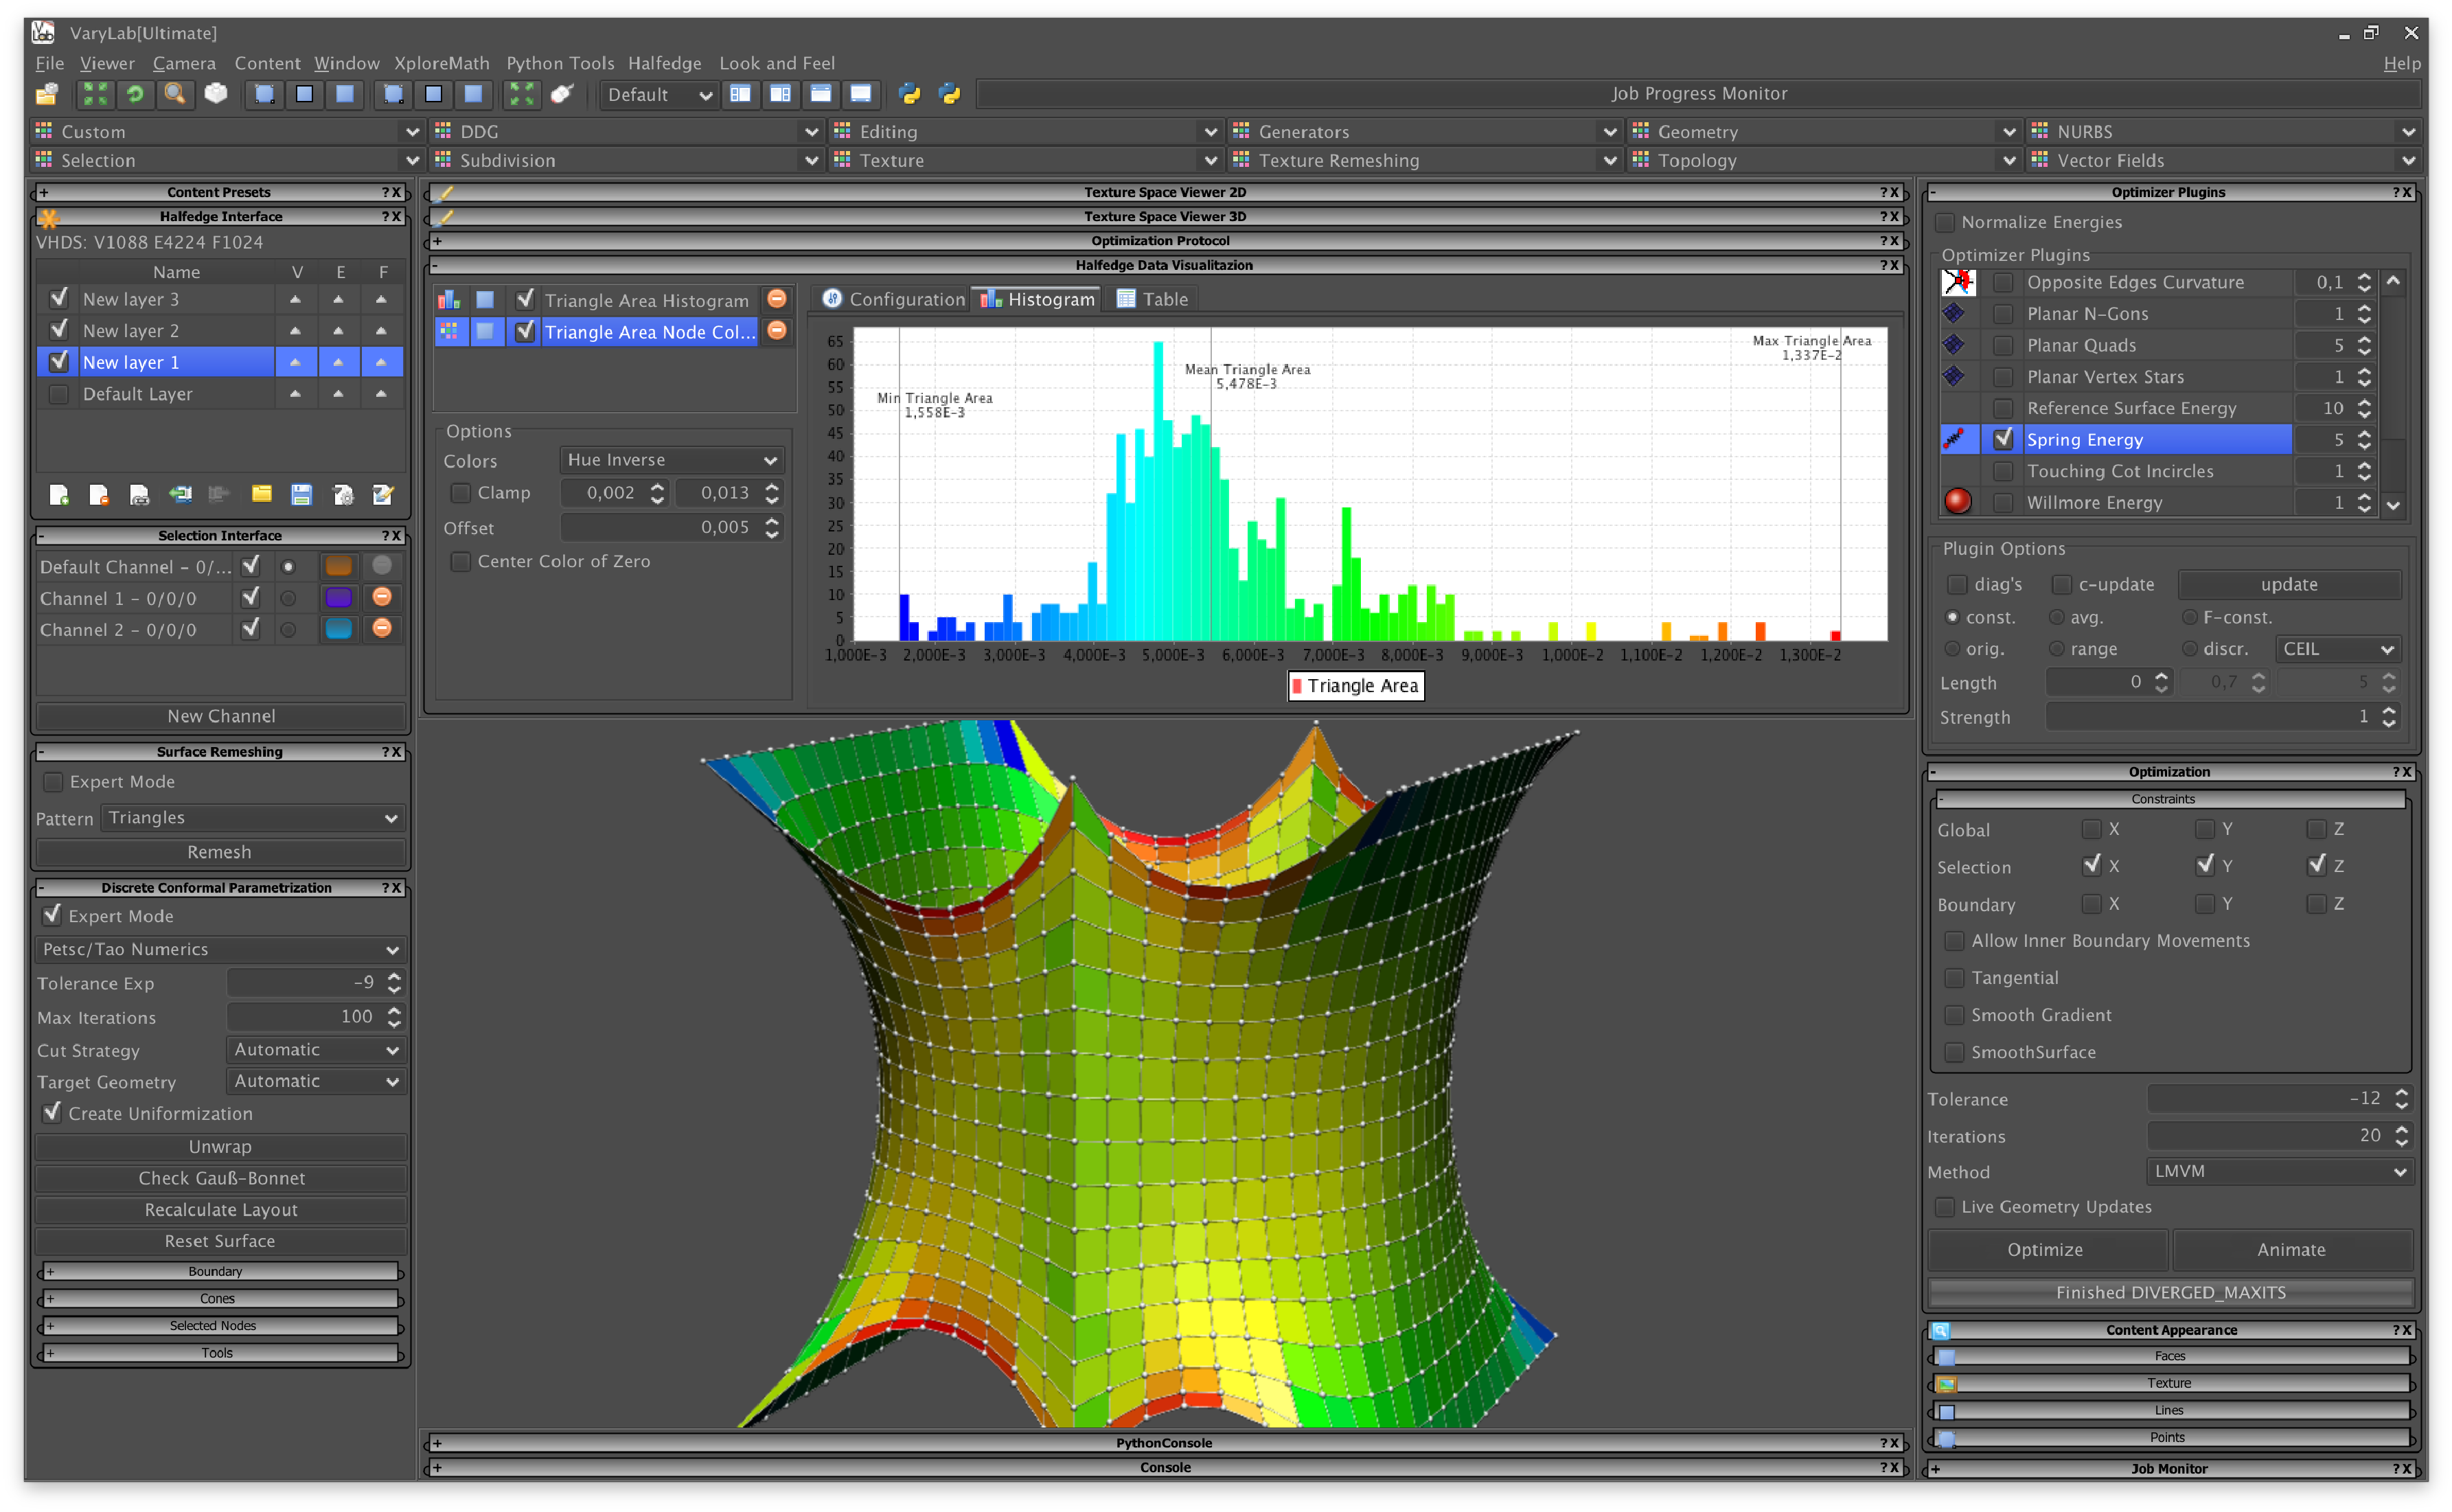
\includegraphics[width=\textwidth]{varylab/varylab_main.pdf}
    \caption{{\sc VaryLab} main user interface window. Visualization interface (top), energy configuration and optimization tools (right), layers, selections, etc. (left).}
    \label{fig:varylab_main_ui}
    \end{center}
\end{figure}

In this chapter we introduce the {\sc Java} software {\sc VaryLab}. 
It is a software developed at Berlin Institute of Technology by the author of this thesis, Thilo R\"orig, and others. 
The software has been developed in the Projects A01 "Discrete Riemann Surfaces" and A08 "Discrete Geometric Structures Motivated by Applications in Architecture" of the SFB Transregio 109 - Discretization in Geometry and Dynamics~\cite{sfb-webpage}.
It is designed to be an extensible and modular tool for experiments with discrete surfaces in pure mathematics and applications in industrial geometry. 
The purpose of this chapter is to enable the reader to reproduce the results presented in Part~\ref{part:applications} of this work.

We start with a general description of {\sc VaryLab} and its features in Section~\ref{sec:general_varylab}. Section~\ref{sec:ui_varylab} introduces the user interface which is based on {\sc JRWorkspace}, see Chapter~\ref{chp:jrworkspace}. Section~\ref{sec:periodic_varylab}, gives details on the use of {\sc VaryLab} when calculating the examples of Chapter~\ref{chp:periodic_conformal_maps}. Section~\ref{sec:quasiisothermic_varylab} explains the steps needed to reproduce results presented in Chapter~\ref{chp:quasiisothermic}. Finally, in Section~\ref{sec:gridshells_varylab} we present the capabilities of {\sc VaryLab} when calculating gridshell nets as explained in Chapter~\ref{chp:gridshells}.

%In this chapter words in [Brackets] describe ui elements.

\section{Non-linear discrete surface optimization}
\label{sec:general_varylab}
In its core, {\sc VaryLab} is a solver for non-linear optimization problems on the coordinates of a given 3D discrete surface. 
That means, given a surface $S$ and functionals $f_1,\ldots,f_n:S\to\R$ we (try to) minimize the combined functional

\begin{eqnarray}
	f(S) = \sum_{i=1}^n \lambda_i f_i(S) \label{eq:varylab_functional}
\end{eqnarray}
where $\lambda_1,\ldots,\lambda_n\in \R$ are user-defined weights. Correspondingly the first and second  derivatives of $f_i(S)$ are weighted by $\lambda_i$
\begin{eqnarray}
	\nabla f(S) = \sum_{i=1}^n \lambda_i \nabla f_i(S), \quad \nabla\nabla f(S) = \sum_{i=1}^n \lambda_i \nabla\nabla f_i(S). \label{eq:varylab_derivatives}
\end{eqnarray}

{\sc VaryLab} uses the numerical library {\sc PETSc}/{\sc TAO} \cite{petsc-user-ref, petsc-web-page, tao-user-ref} and the corresponding {\sc Java} bindings \cite{jpetsctao-web-page} for computations. To run optimization methods we need at least an implementation of the functional's value. Other methods need the gradient or Hessian of the functional. The most important methods are
 
\begin{tabular}{l | l | l}
\multicolumn{1}{c|}{$f$} & \multicolumn{1}{c|}{$f$, $\nabla f$} & \multicolumn{1}{c}{$f$, $\nabla f$, $\nabla\nabla f$}\\
\hline
{\tt NM} Nelder-Mead & {\tt LMVM} Limited-Memory, Variable-Metric & {\tt NLS} Newton Line-Search \\
& {\tt CG} Conjugate Gradient & {\tt NTR} Newton Trust-Region.
\end{tabular}

In {\sc VaryLab} a functional can choose to implement just the value. Additionally it can implement the gradient and the Hessian of $S$. In principle all methods can be used with all functionals even if those do not implement all data needed for the algorithm. {\sc VaryLab} approximates the values of the gradient or the Hessian if they are missing.

{\sc VaryLab} has the option to normalize the energies before optimization and calculates a $\mu_i$ for each of the energies such that 	$\left\Vert\mu_i\nabla f_i(S)\right\Vert = 1$ for each functional $f_i$ and for the current mesh geometry. Then it uses a modified energy
\begin{eqnarray}
	\hat{\mathit f}(S) = \sum_{i=1}^n \mu_i\lambda_i f_i(S). \label{eq:varylab_normalized_functional}
\end{eqnarray}
for optimization.

{\sc VaryLab} can handle constraints on vertex positions. We implement this by modifying the gradient and Hessian of the selected energies to be zero at the constraint variables. Even if the derivative does not match the energy anymore, we can still calculate solutions for the rest of the variables using conjugate gradient methods. Here the line search step of the algorithm minimizes the energy over the remaining variables in the direction of the gradient, i.e., the update will not include constraint variables.

\section{Built-in functionals}

{\sc VaryLab} implements a number of energy functionals that are implemented as {\sc JRworkspace} plug-ins and can be selected in the \emph{Optimizer Plug-ins} panel.

\begin{compactitem}[$\bullet$]
\item \emph{Circular Quadrilaterals Energy} - Defines an energy functional that is minimal for planar circular quads. Since we are using an angle criterion, the convergence to planarity is relatively slow. If the \emph{Planar Quadrilaterals} energy is added to the optimization, the geometry converges more quickly.
\item \emph{Conical Quadrilaterals Energy} - This energy implements an angle criterion for conical meshes. In combination with \emph{Planar Quadrilaterals} or \emph{Planar n-gons} it optimizes a mesh to have the property that faces adjacent to a vertex are tangent to a cone of revolution.
\item \emph{Cotangent Dirichlet Energy} - Dirichlet energy for the three coordinate functions of vertices of a triangle mesh. Edge weights are defined as $\omega_\mathit{ij}=\frac{1}{2}(\cot\alpha_\mathit{ij}+\cot\alpha_\mathit{ji})$ where $\alpha_\mathit{ij}$ and $\alpha_\mathit{ji}$ are the angles opposite of the edge $e_\mathit{ij}$.
\item \emph{Equal Edge Lengths} - This energy penalizes the deviation of edge lengths from their mean value. As a result it is minimal, if all edges have the same length.
\item \emph{Incircles} - The property for a quadrilateral to possess an incircle tangent to its sides is that the two sums of opposite side lengths are equal, i.e., $a+c=b+d$. Planarity is not included in this functional, so to get planar quadrilaterals with inscribed incircles one needs to add planarity to the optimization.
\item \emph{Touching Incircles} - In a quad-mesh with incircles, the incircles need not touch. In combination with the \emph{Incircles} and \emph{Planarity} energies one can create a meshes with touching incircles.
\item \emph{Opposite Edges Curvature} - This energy penalizes the deviation of a parameter poly-line from a straight line. Using this energy alone, will move the mesh towards a discrete ruled surface. Used together with, e.g., a \emph{Reference Mesh} energy, this energy smoothes the  parameter lines of a quad-mesh.
\item \emph{Opposite Angles Curvature} - This curvature is based on the intrinsic geometry of the surface. Let $\alpha$, $\beta$, $\gamma$, and $\delta$ denote the angles in the adjacent quads at a node in cyclic order. Then the optimal mesh satisfies $\alpha+\beta=\gamma+\delta$ and $\beta+\gamma=\delta+\alpha$, i.e., the parameter lines are straight from an intrinsic point of view.
\item \emph{Planar Quadrilaterals} - Energy that enforces planarity of quadrilaterals. Implemented either as the distance of the diagonals or as the determinant of the four homogeneous vertex coordinates.
\item \emph{Planar $n$-gons} - Generalization of the energy for planar quadrilaterals. Implemented as the sum of all choices of four vertices in each face.
\item \emph{Planar Vertex Stars} - This energy is dual to the planar faces energy. It computes the volume spanned by a node and its neighbors. Minimization yields meshes such that each node lies in a plane with its neighbors. If used together with face planarity, the initial mesh is mapped to a plane.
\item \emph{Reference Mesh} - Given a reference mesh we compute the closest point to a node and add a spring force between each node and its projection. The projection point is recomputed in each step of the optimization. If combined with other energies, it keeps the optimized mesh close to a reference mesh.
\item \emph{Spring Energy} - The spring energy is computed by adding springs to all the edges of the mesh. These springs can have user-specified target lengths and strengths that can be specified by various options.
\end{compactitem}

\section{Geometry processing}

The geometry processing core of {\sc VaryLab} is based on {\sc HalfEdge} and {\sc HalfEdgeTools} (Chapter~\ref{chp:halfedge}), i.e., all geometry processing is done with the help of the half-edge data structure and algorithms that run on top of it. Frequently used geometry processing features include

\begin{figure}
    \begin{center}
    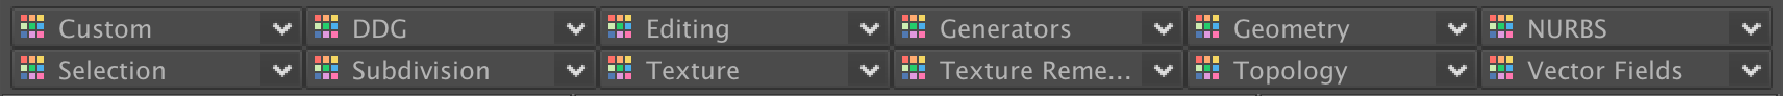
\includegraphics[width=\textwidth]{varylab/tools.pdf}
    \caption{{\sc VaryLab} tools tool bar.}
    \label{fig:varylab_tools_ui}
    \end{center}
\end{figure}

\begin{compactitem}[$\bullet$]
\item Mesh Generators - Regular Planar Meshes, Convex Hull, Primitive Meshes such as cube, cylinder, sphere, etc.
\item Mesh Editing - Vertex/Edge/Face operations based on user selection.
\item Subdivision - Catmull-Clark, Doo-Sabin, Loop, Sqrt3, etc.
\item Remeshing - Quadrilaterals, Triangles, Singularities.
\end{compactitem}

All tools are available via the tools tool bar at the top of the main window, see Figure~\ref{fig:varylab_main_ui} and~\ref{fig:varylab_tools_ui}.

\section{Data visualization}

{\sc VaryLab} adds data sources corresponding to the energies of the optimization core. Their data can be visualized on the surface using the \emph{Halfedge Data Visualization} interface, see Section~\ref{sec:halfedge_tools_visualization}. 

\begin{figure}
    \begin{center}
    \resizebox{\textwidth}{!}{
        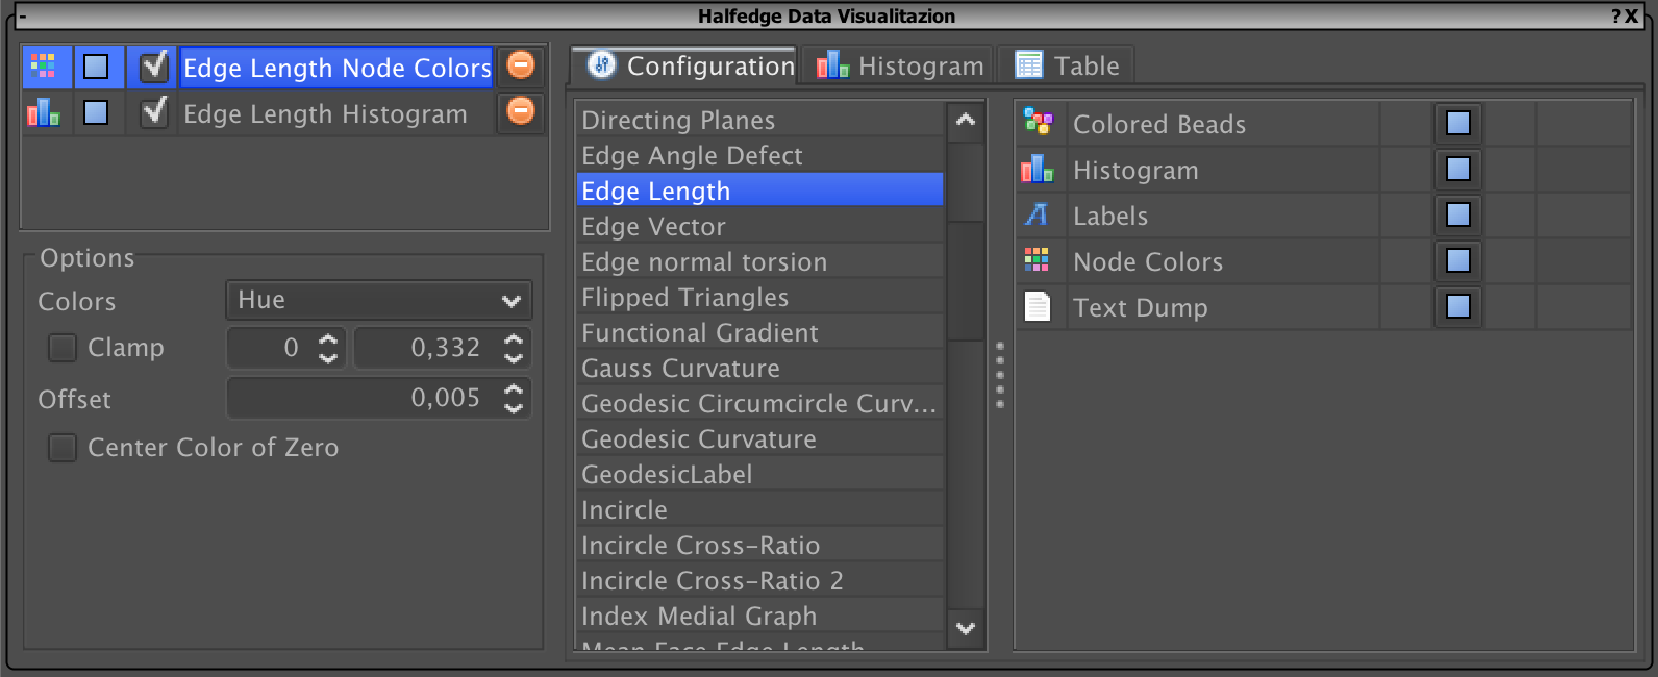
\includegraphics[width=\textwidth]{varylab/edge_visualization.pdf}
        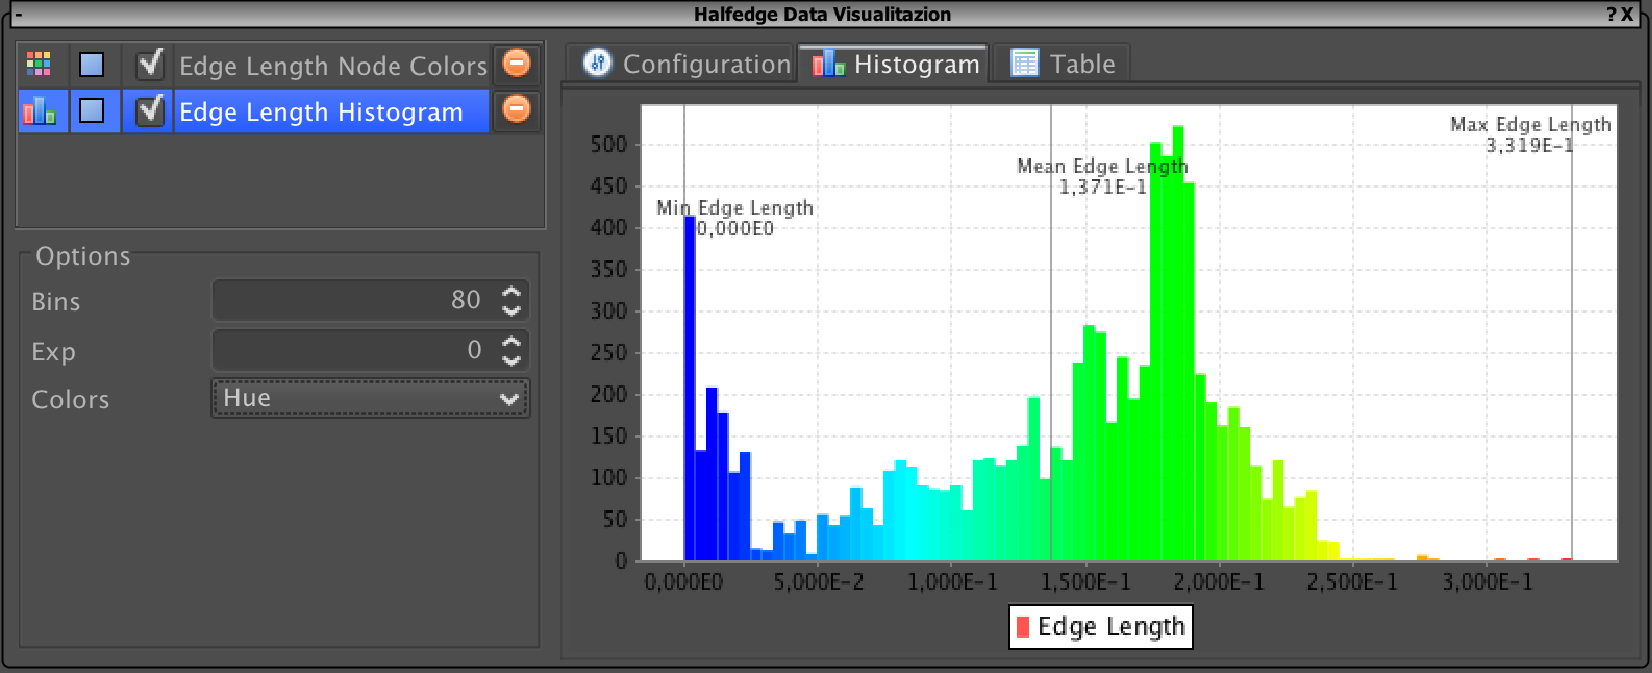
\includegraphics[width=\textwidth]{varylab/edge_histogram.pdf}    
    }
    \caption{Visualization interface (left), Visualizing mesh edge length data as node colors on a surface and as histogram (right).}
    \label{fig:visualizing_edge_lengths}
    \end{center}
\end{figure}

{\bf Example: analyzing edge length distribution.}
\nopagebreak

Load a mesh geometry. In the \emph{Halfedge Data Visualization} select the \emph{Edge Length} data source. It provides scalar data for edges of the mesh. Select the \emph{Histogram} and \emph{Node Colors} visualizers to create colored edges and a corresponding histogram for the edge lengths of the mesh, see Figure~\ref{fig:visualizing_edge_lengths}.


\section{User interface}
\label{sec:ui_varylab}

The user interface of {\sc VaryLab}, see Figure~\ref{fig:varylab_main_ui}, is based on {\sc JRWorkspace}, Chapter~\ref{chp:jrworkspace}. Thus it inherits the ability for the user to freely move around all interface components of the main window, see Figure~\ref{fig:varylab_main_ui}. 
The three most important interface components are shown in Figure~\ref{fig:optimization_interface_varylab} and \ref{fig:protocol_interface_varylab}. It is the list of energies, the optimization controls, and the optimization protocol.

\begin{figure}
\begin{center}
    \resizebox{\linewidth}{!}{
        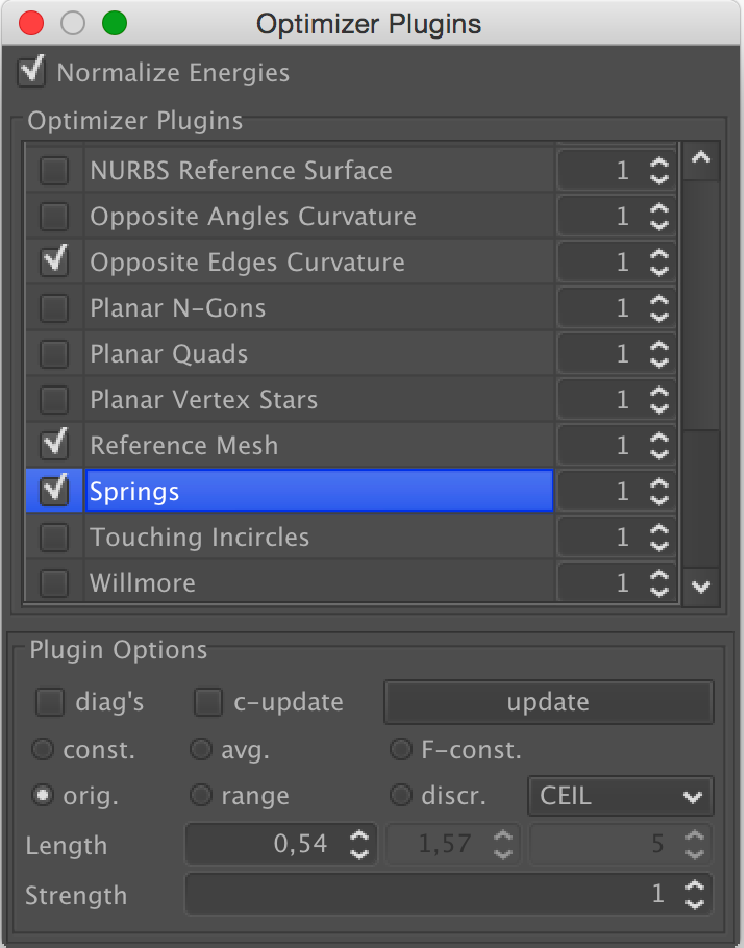
\includegraphics[width=\textwidth]{varylab/optimization_plugins2.pdf}
        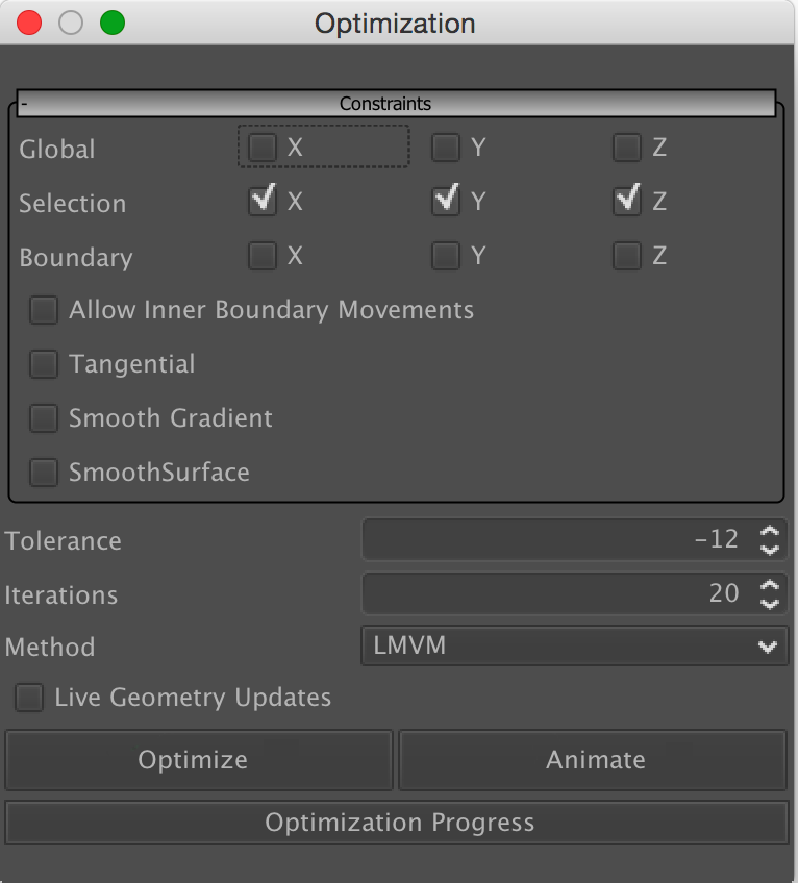
\includegraphics[width=\linewidth]{varylab/optimization2.pdf}
    }
\caption{The main user interface panels of {\sc VaryLab}. List of optimization functional plug-ins and their options (left). Main optimization controls with global constraints and minimizer settings (right).}
\label{fig:optimization_interface_varylab}
\end{center}
\end{figure}

\subsection*{Optimizer Plug-ins Panel}
The \emph{Optimizer Plugins} panel, see Figure~\ref{fig:optimization_interface_varylab} (left), has a list with all currently loaded plug-ins that implement energies for the use with the non-linear optimization core. For each energy one can adjust the coefficient $\lambda$ in the sum of functionals, see Equation~(\ref{eq:varylab_functional}).
The checkbox \emph{Normalize Energies} activates normalization of energies, see Equation~(\ref{eq:varylab_normalized_functional}). For a selected energy, options are displayed right under the table.

\subsection*{Optimization Panel}
In the \emph{Optimization Panel}, see Figure~\ref{fig:optimization_interface_varylab} (right), we can configure constraints and run the optimization. Vertices can be fixed either globally in one or all coordinate directions, by selection, or as boundary constraint. Constraints are handled as described in Section~\ref{sec:general_varylab}

The check box \emph{Allow Inner Boundary Movement} is used in conjunction with boundary constraints. The corresponding gradient part is projected onto an adjacent boundary edge thus any conjugate gradient update will move the vertex along this direction. This mode is meant to be used with straight boundaries, otherwise the behavior is undefined.

Analog to the inner boundary movement constraint, the \emph{Tangential}
 constraint projects the gradient of a vertex onto the tangent plane at this vertex for current mesh geometry. With this option, vertices stay close to the initial surface if the surface is sufficiently smooth but can move freely along tangent directions of the surface.

The options \emph{Smooth Gradient} and \emph{Smooth Surface} apply Laplacian smoothing to either the gradient or the coordinate values of the mesh. We use a graph Laplacian, i.e., all weights are equal to 1.

The values for \emph{Tolerance} and \emph{Iterations} define stop criteria for the optimization core. If the Frobenius norm of the gradient drops below the tolerance or if the maximum number of iterations are performed, the optimizer stops. 

The numerical \emph{Method} can be selected from the drop down field, see Section~\ref{sec:general_varylab} for explanation.

The check box \emph{Live Geometry Updates} updates the coordinates of the surface during optimization if selected. Any visualization is updated accordingly.

\subsection*{Optimization Protocol Panel}

During optimization {\sc VaryLab} logs the energy of each functional as well as the Frobenius norm of the gradient and plots them to the optimization protocol, see Figure~\ref{fig:protocol_interface_varylab}. The energy value is drawn as a green curve, the norm of the gradient is a purple curve. By default the display is logarithmic in the values and linear in time.

\begin{figure}
\begin{center}
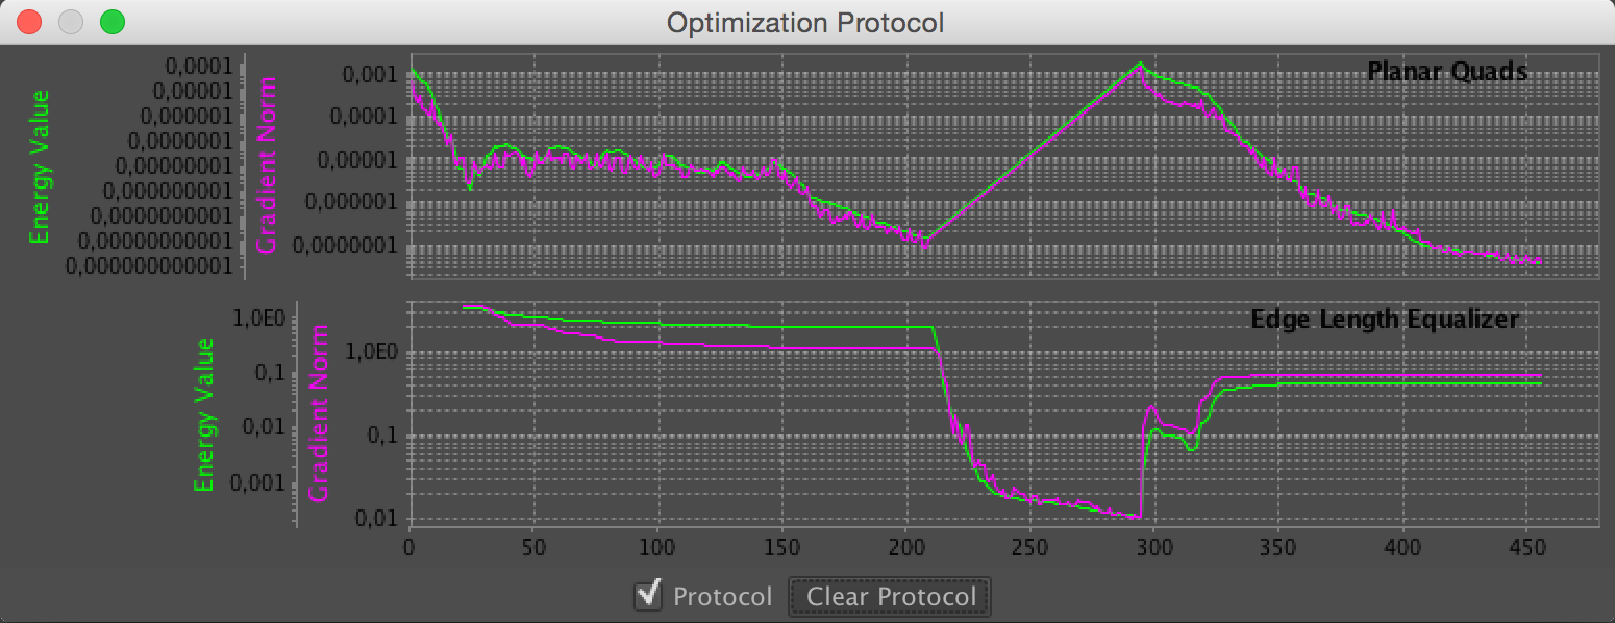
\includegraphics[width=\textwidth]{varylab/protocol.pdf}
\caption{Optimization protocol panel shows the progress of the optimization for each activated energy in the Optimizer Plug-ins panel, see Figure~\ref{fig:optimization_interface_varylab} (left).}
\label{fig:protocol_interface_varylab}
\end{center}
\end{figure}

\section{Periodic conformal maps with {\sc VaryLab}}
\label{sec:periodic_varylab}
In this section we describe how the methods of Chapter~\ref{chp:periodic_conformal_maps} are implemented in {\sc VaryLab}. We split the process in two parts. Part one describes the creation of periodic triangle, quad, or hexagonal meshes from an initial unstructured triangle mesh. Part two deals with optimization of panels created from a mesh in part one.

\subsection{Periodic parameterization}
The parameterization part of the work is carried out via the {\sc ConformalLab} main user interface. 

\begin{compactenum}[(1)]
\item[(0)] We load a surface with two boundary components. We can map the surface to a pattern-adapted cone of revolution using the three methods described in Chapter~\ref{chp:periodic_conformal_maps}: mapping to a cylinder (a), polygonal map to a cone of revolution (b), and isometric boundary mapping(c).
\item[(1a)] For the map to the cylinder we create a conformal parameterization with straight boundary using the \emph{Discrete Conformal Parameterization} panel and \emph{Quantized Angles/Straight} boundary mode. A cut is introduced automatically to uniquely define the map.\\

\begin{center}
\begin{minipage}{0.9\linewidth}
            \centering
            \resizebox{\linewidth}{!}{
            	\includegraphics{periodic/step00.pdf}
            	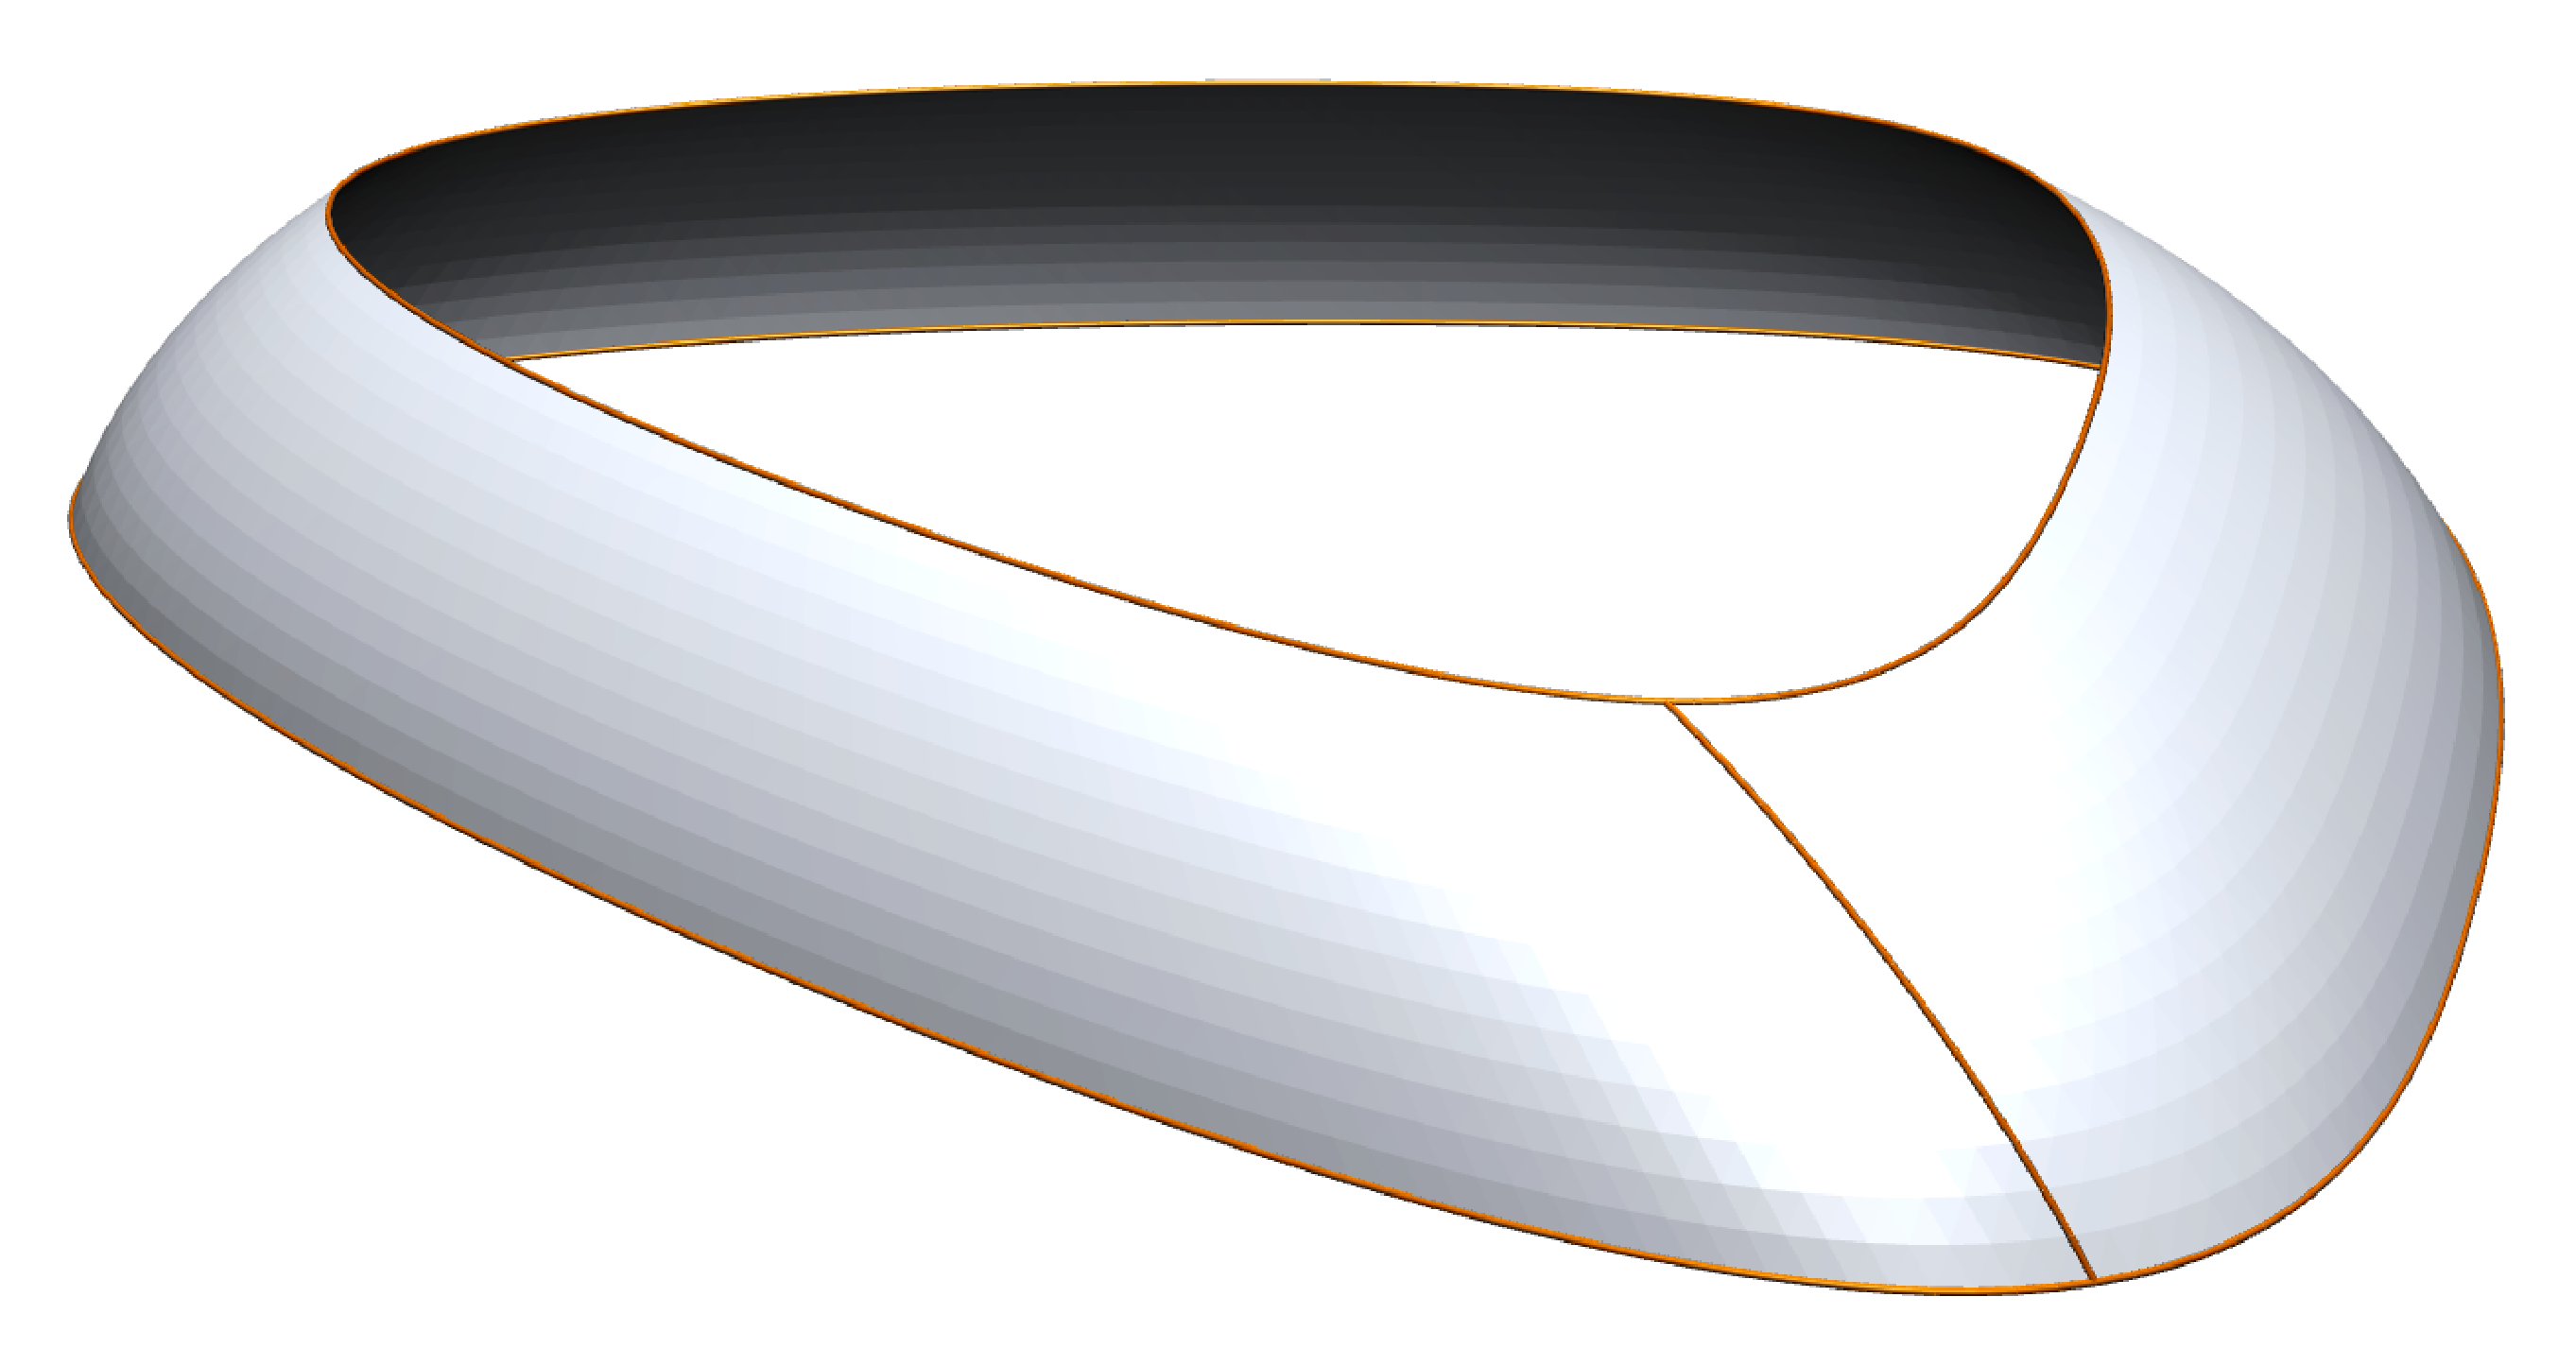
\includegraphics{periodic/step01_surface.pdf}	
            	\includegraphics{periodic/step02_surface.pdf}		
            }
            \resizebox{\linewidth}{!}{
                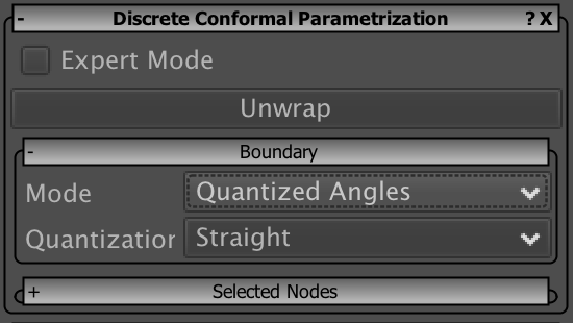
\includegraphics[width=3.2cm]{periodic/step01_ui.pdf}
                \begin{minipage}[b]{10cm}
                    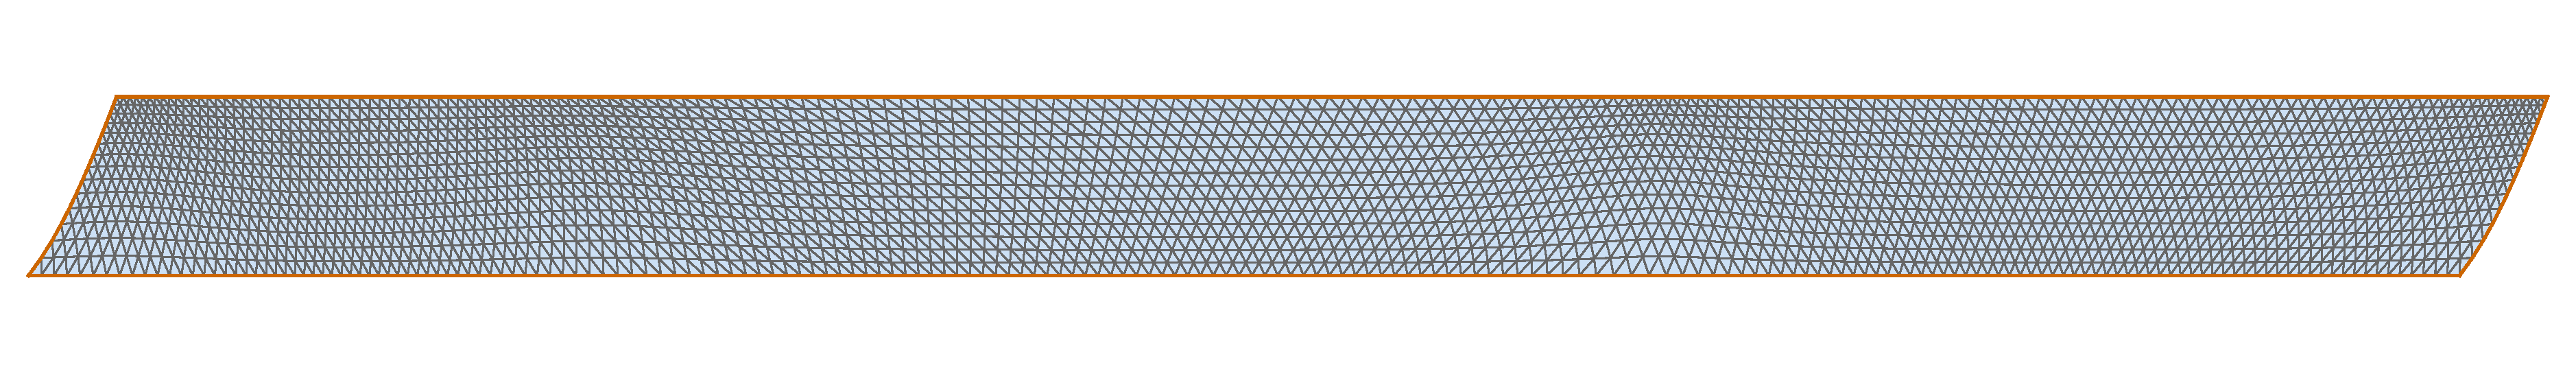
\includegraphics[width=\linewidth]{periodic/step01a_map.pdf}\\
                    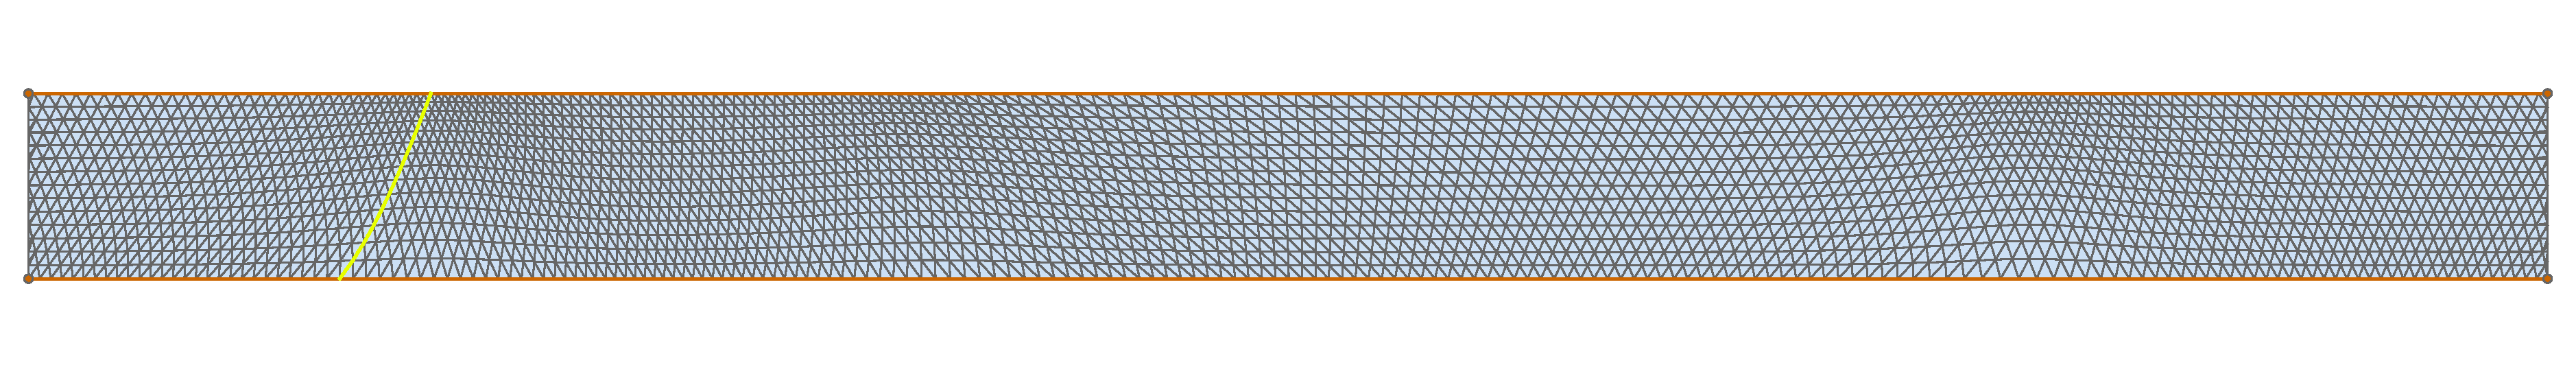
\includegraphics[width=\linewidth]{periodic/step02a_map.pdf}
                \end{minipage}
            }
            \captionof{figure}{Map to cylinder. Start with an automatically cut mesh (top-middle and upper domain image) and modify the cut (top-right and lower domain image) such that the remeshing algorithm can handle the complete boundary.}
            \label{fig:periodic_algorithm1a}
\end{minipage}
\end{center}            

\item[(1b)] For a polygonal map to a cone of revolution, we select boundary vertices to specify boundary angles for the domain. We use multiples of $\frac{\pi}{3}$ for triangle/hexagonal panels and multiples of $\frac{\pi}{4}$ for quadrilaterals.

\begin{center}
\begin{minipage}{0.9\linewidth}
            \centering
            \resizebox{0.7\textwidth}{!}{
            	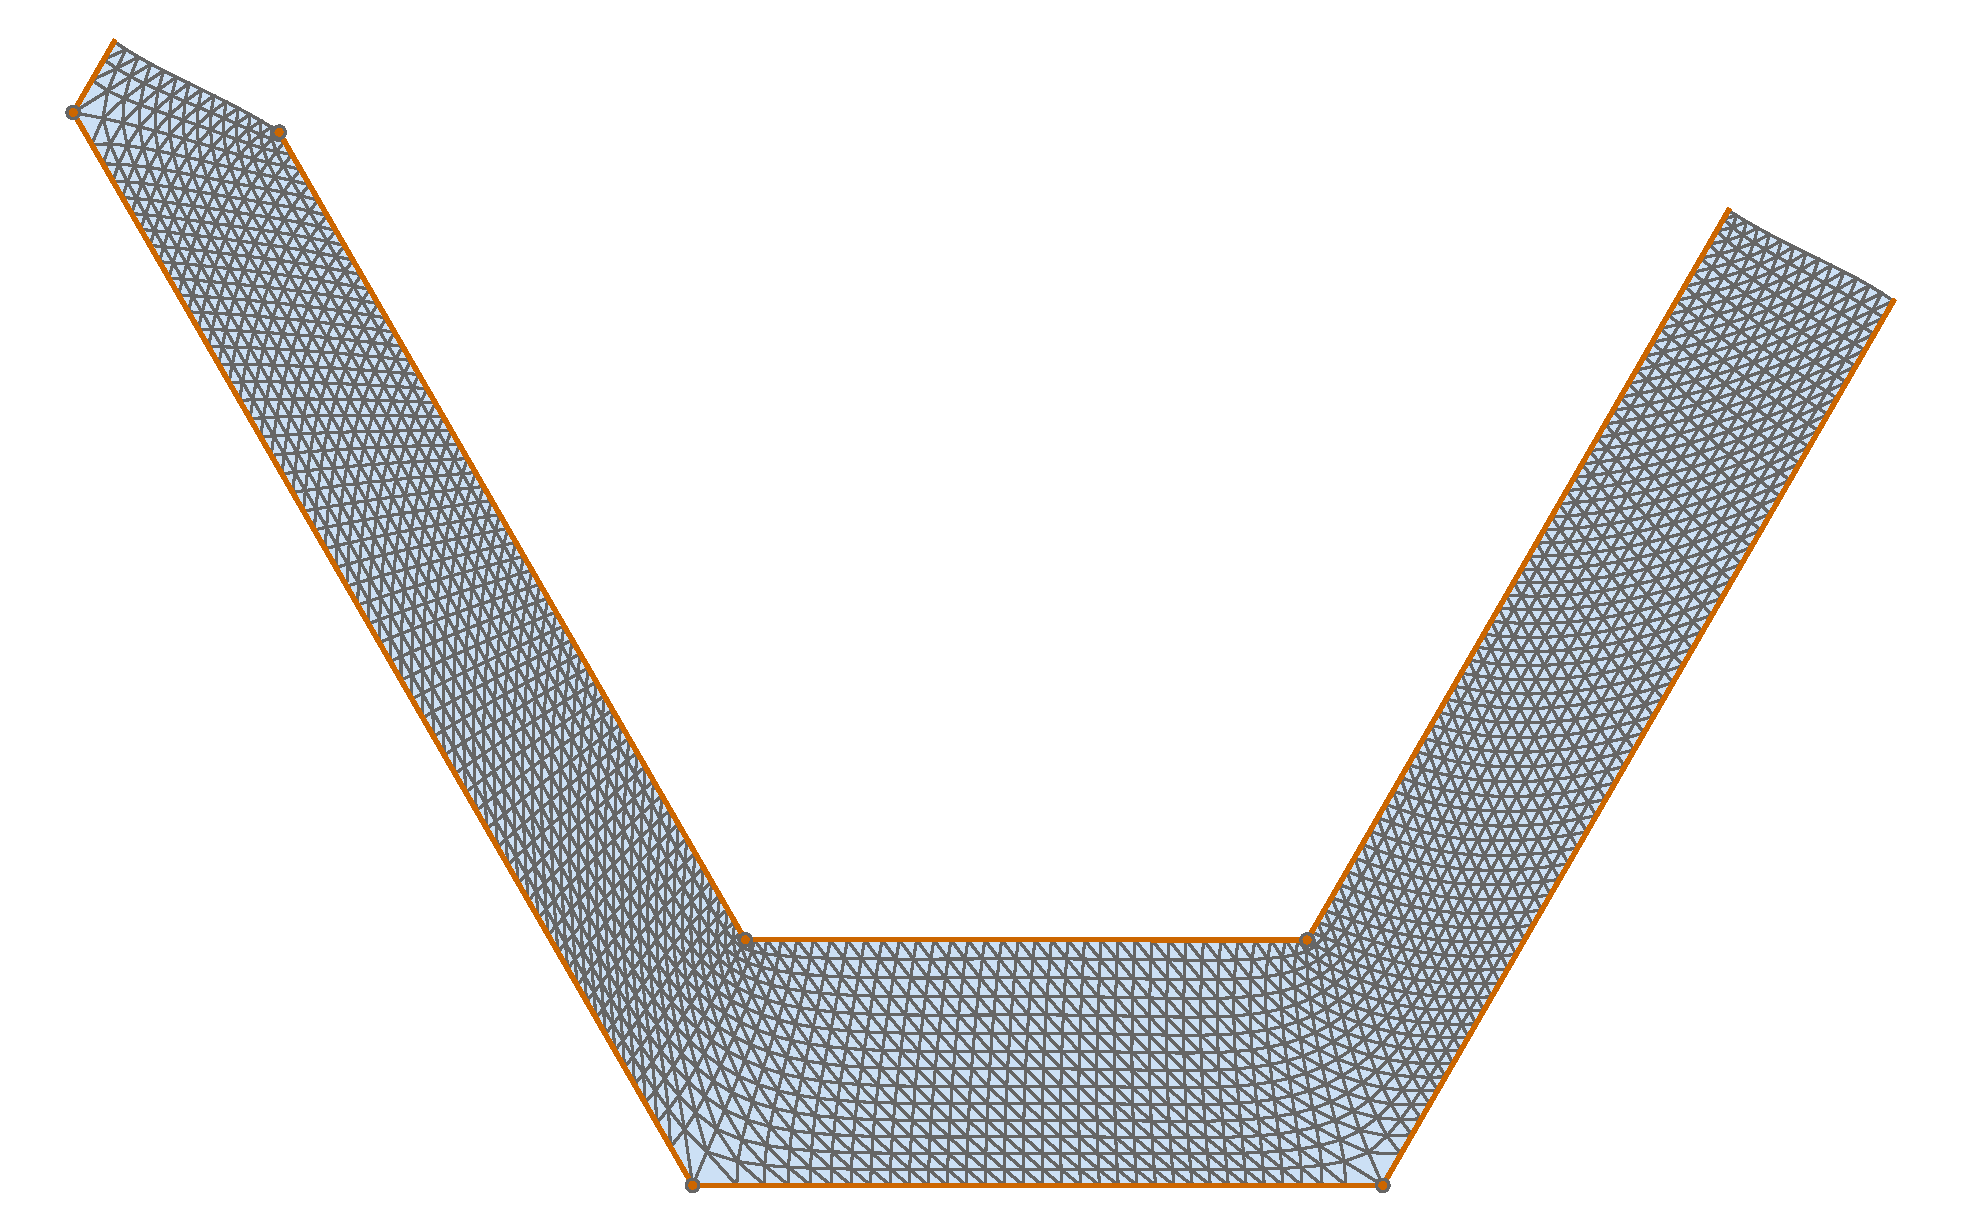
\includegraphics{periodic/step01b_map.pdf}
            	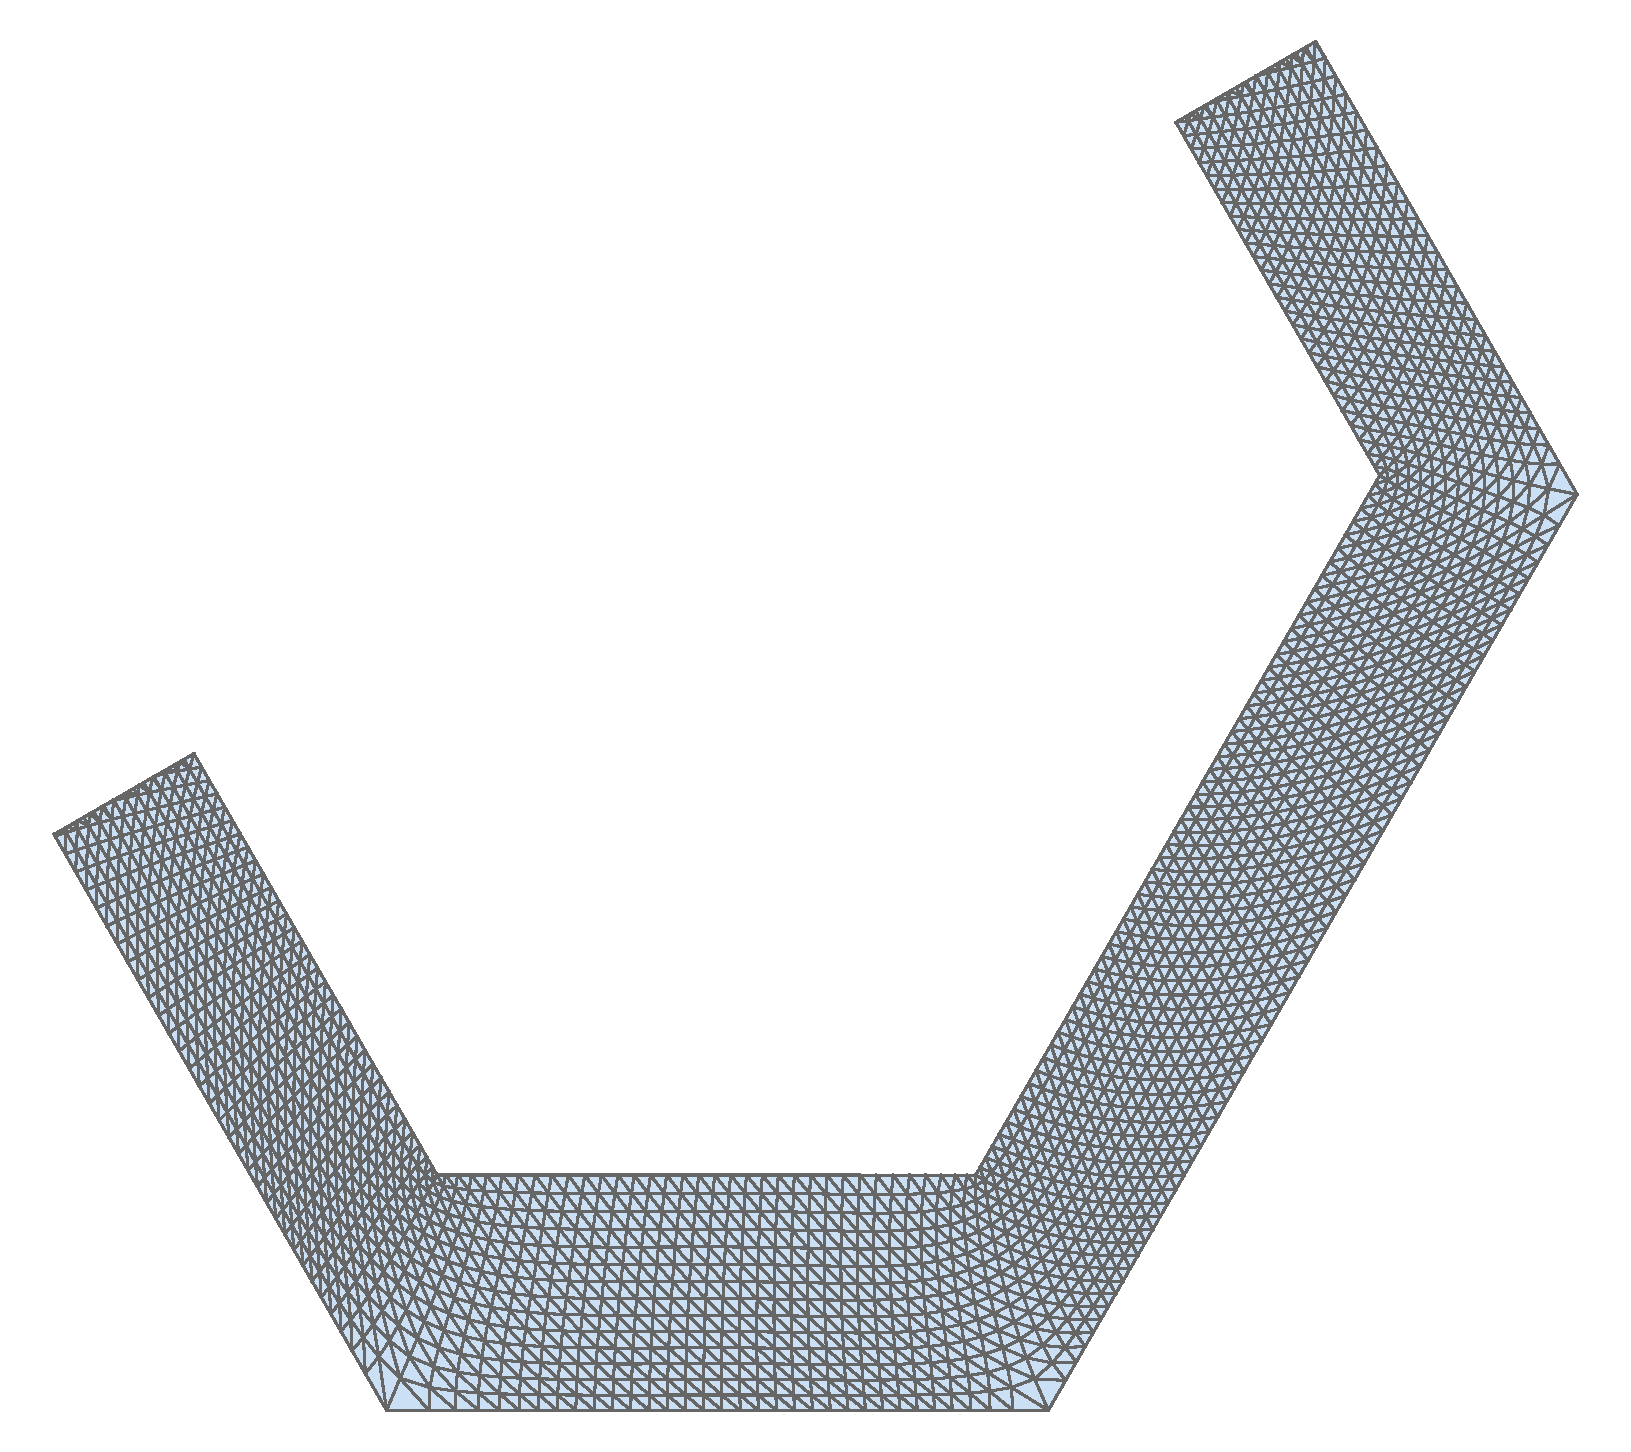
\includegraphics{periodic/step02b_map.pdf}	
            }
            \captionof{figure}{Mapping the surface from Figure~\ref{fig:periodic_algorithm1a} to a hex pattern adapted domain with polygonal boundary curve. Cut orthogonal to the boundary to create a domain that can easily be meshed with boundary-aligned hexagons. The domain is identified along the cut via a rotation by $\pi$.}
\end{minipage}
\end{center}

\item[(1c)] We create an isometric boundary and a map to cone of revolution using the \emph{Read Isometric Angles} boundary mode and the \emph{NoCuts} cut strategy. It creates a map to an arbitrary cone of revolution and reads off the resulting boundary angles. Those are set as new boundary conditions (red vertex selection). In a second step we choose the \emph{Quantized Angle Periods} boundary mode and the desired quantization for the final map to the pattern adapted cone of revolution.

\begin{center}
\begin{minipage}{0.9\linewidth}
            \centering
            \resizebox{\linewidth}{!}{
            	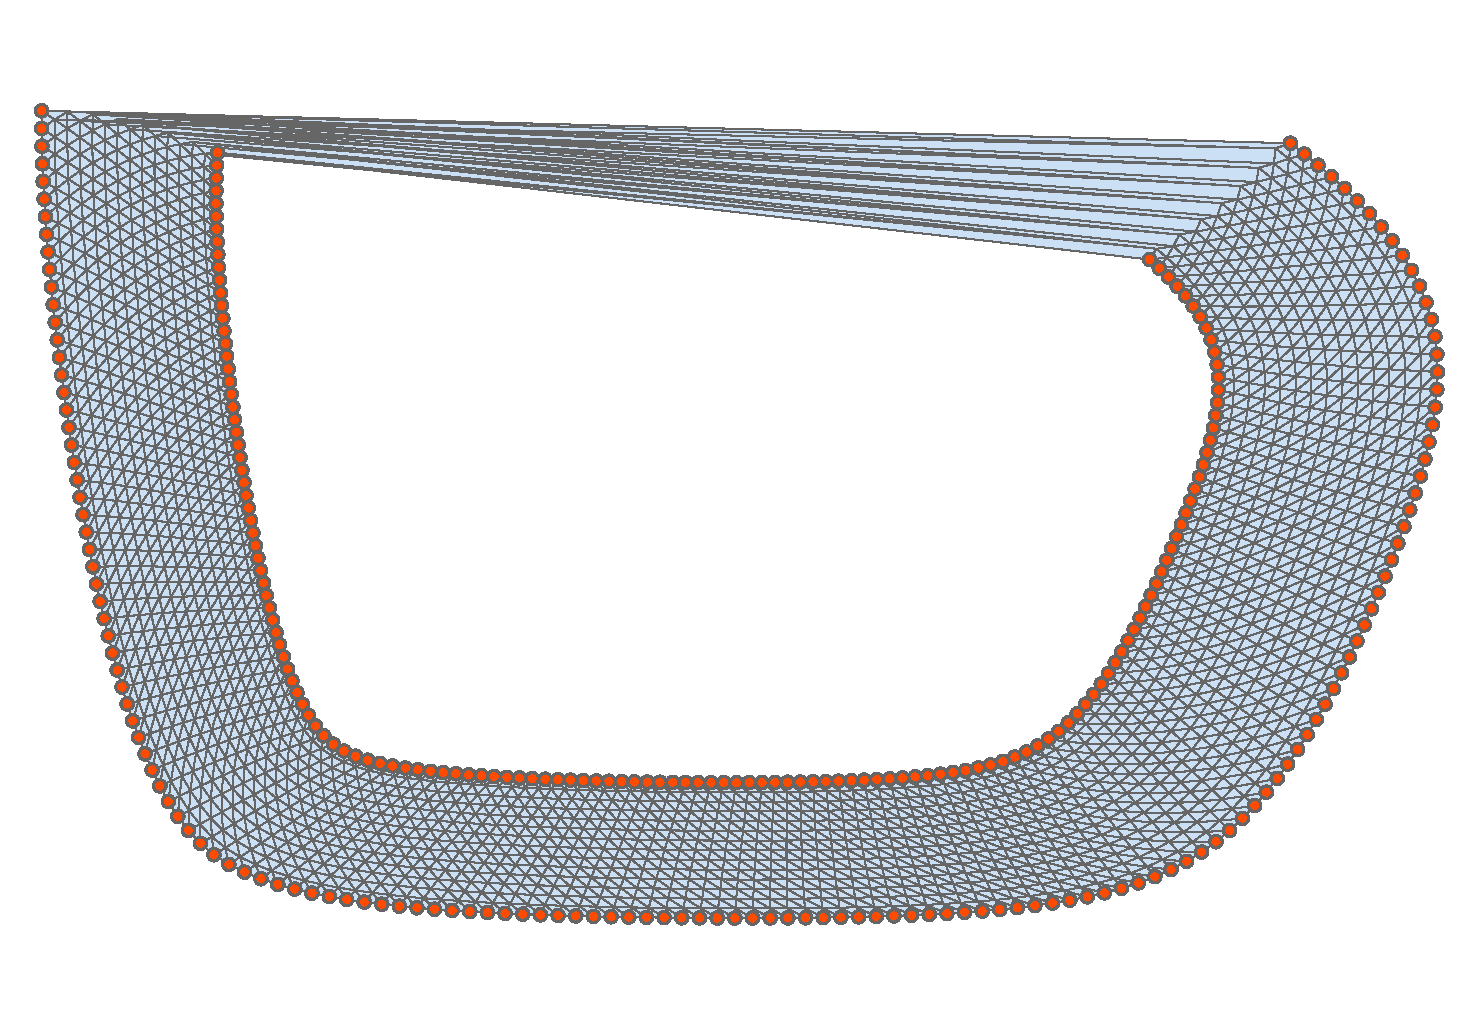
\includegraphics[width=5cm]{periodic/step01c_map.pdf}
            	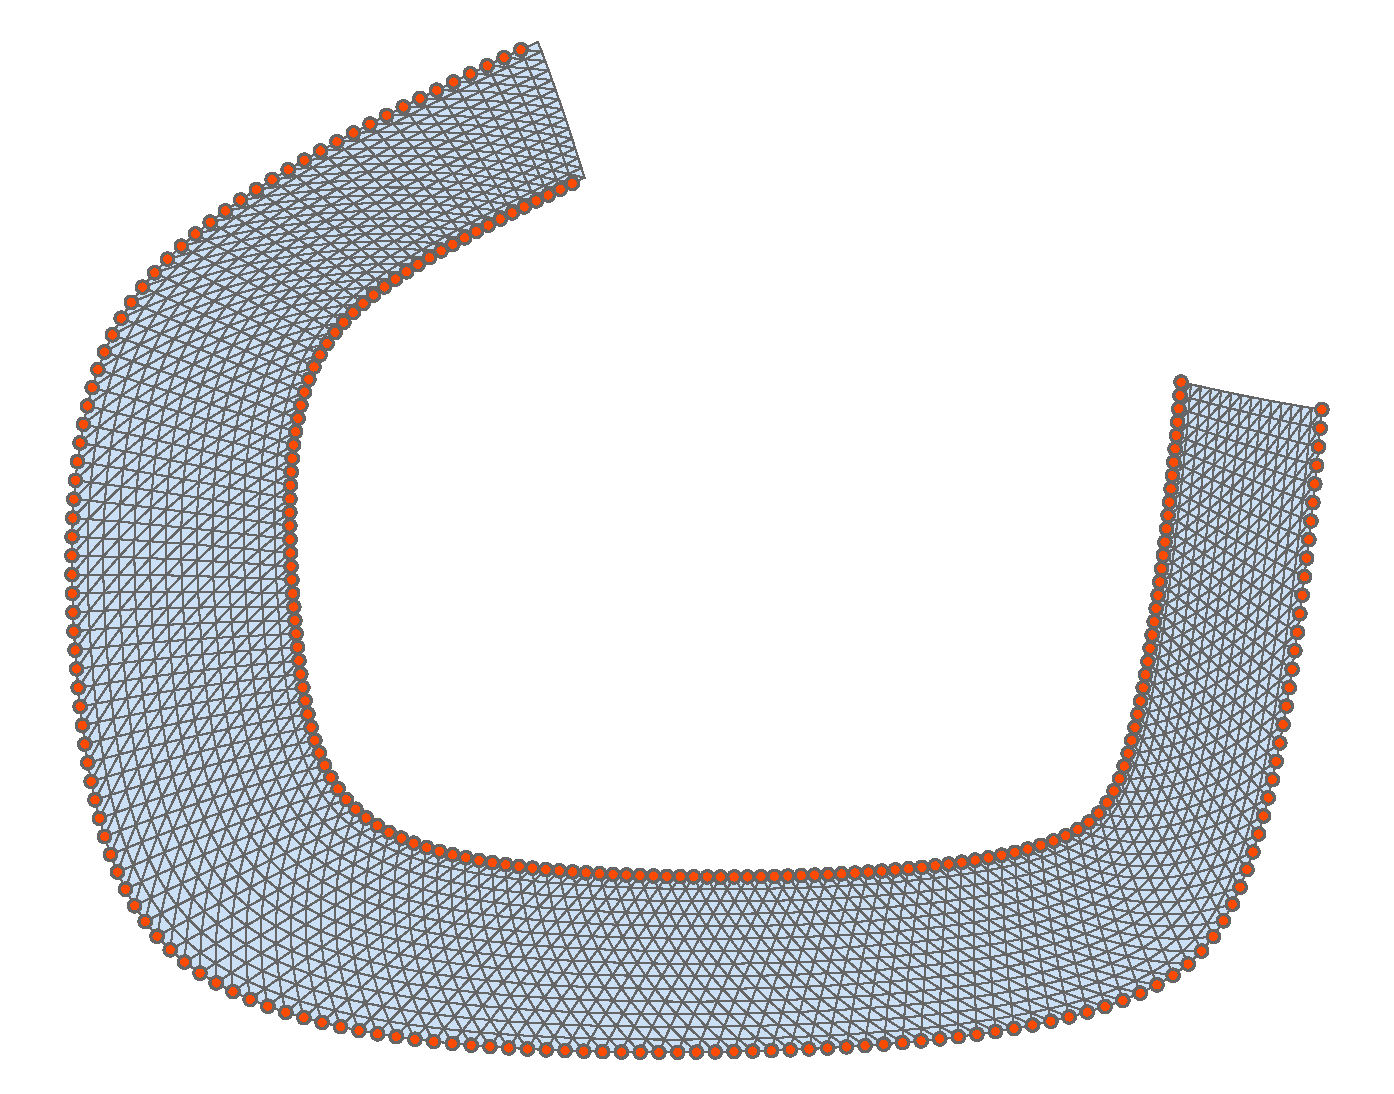
\includegraphics[width=5cm]{periodic/step02c_map_hexadapted.pdf}	
            	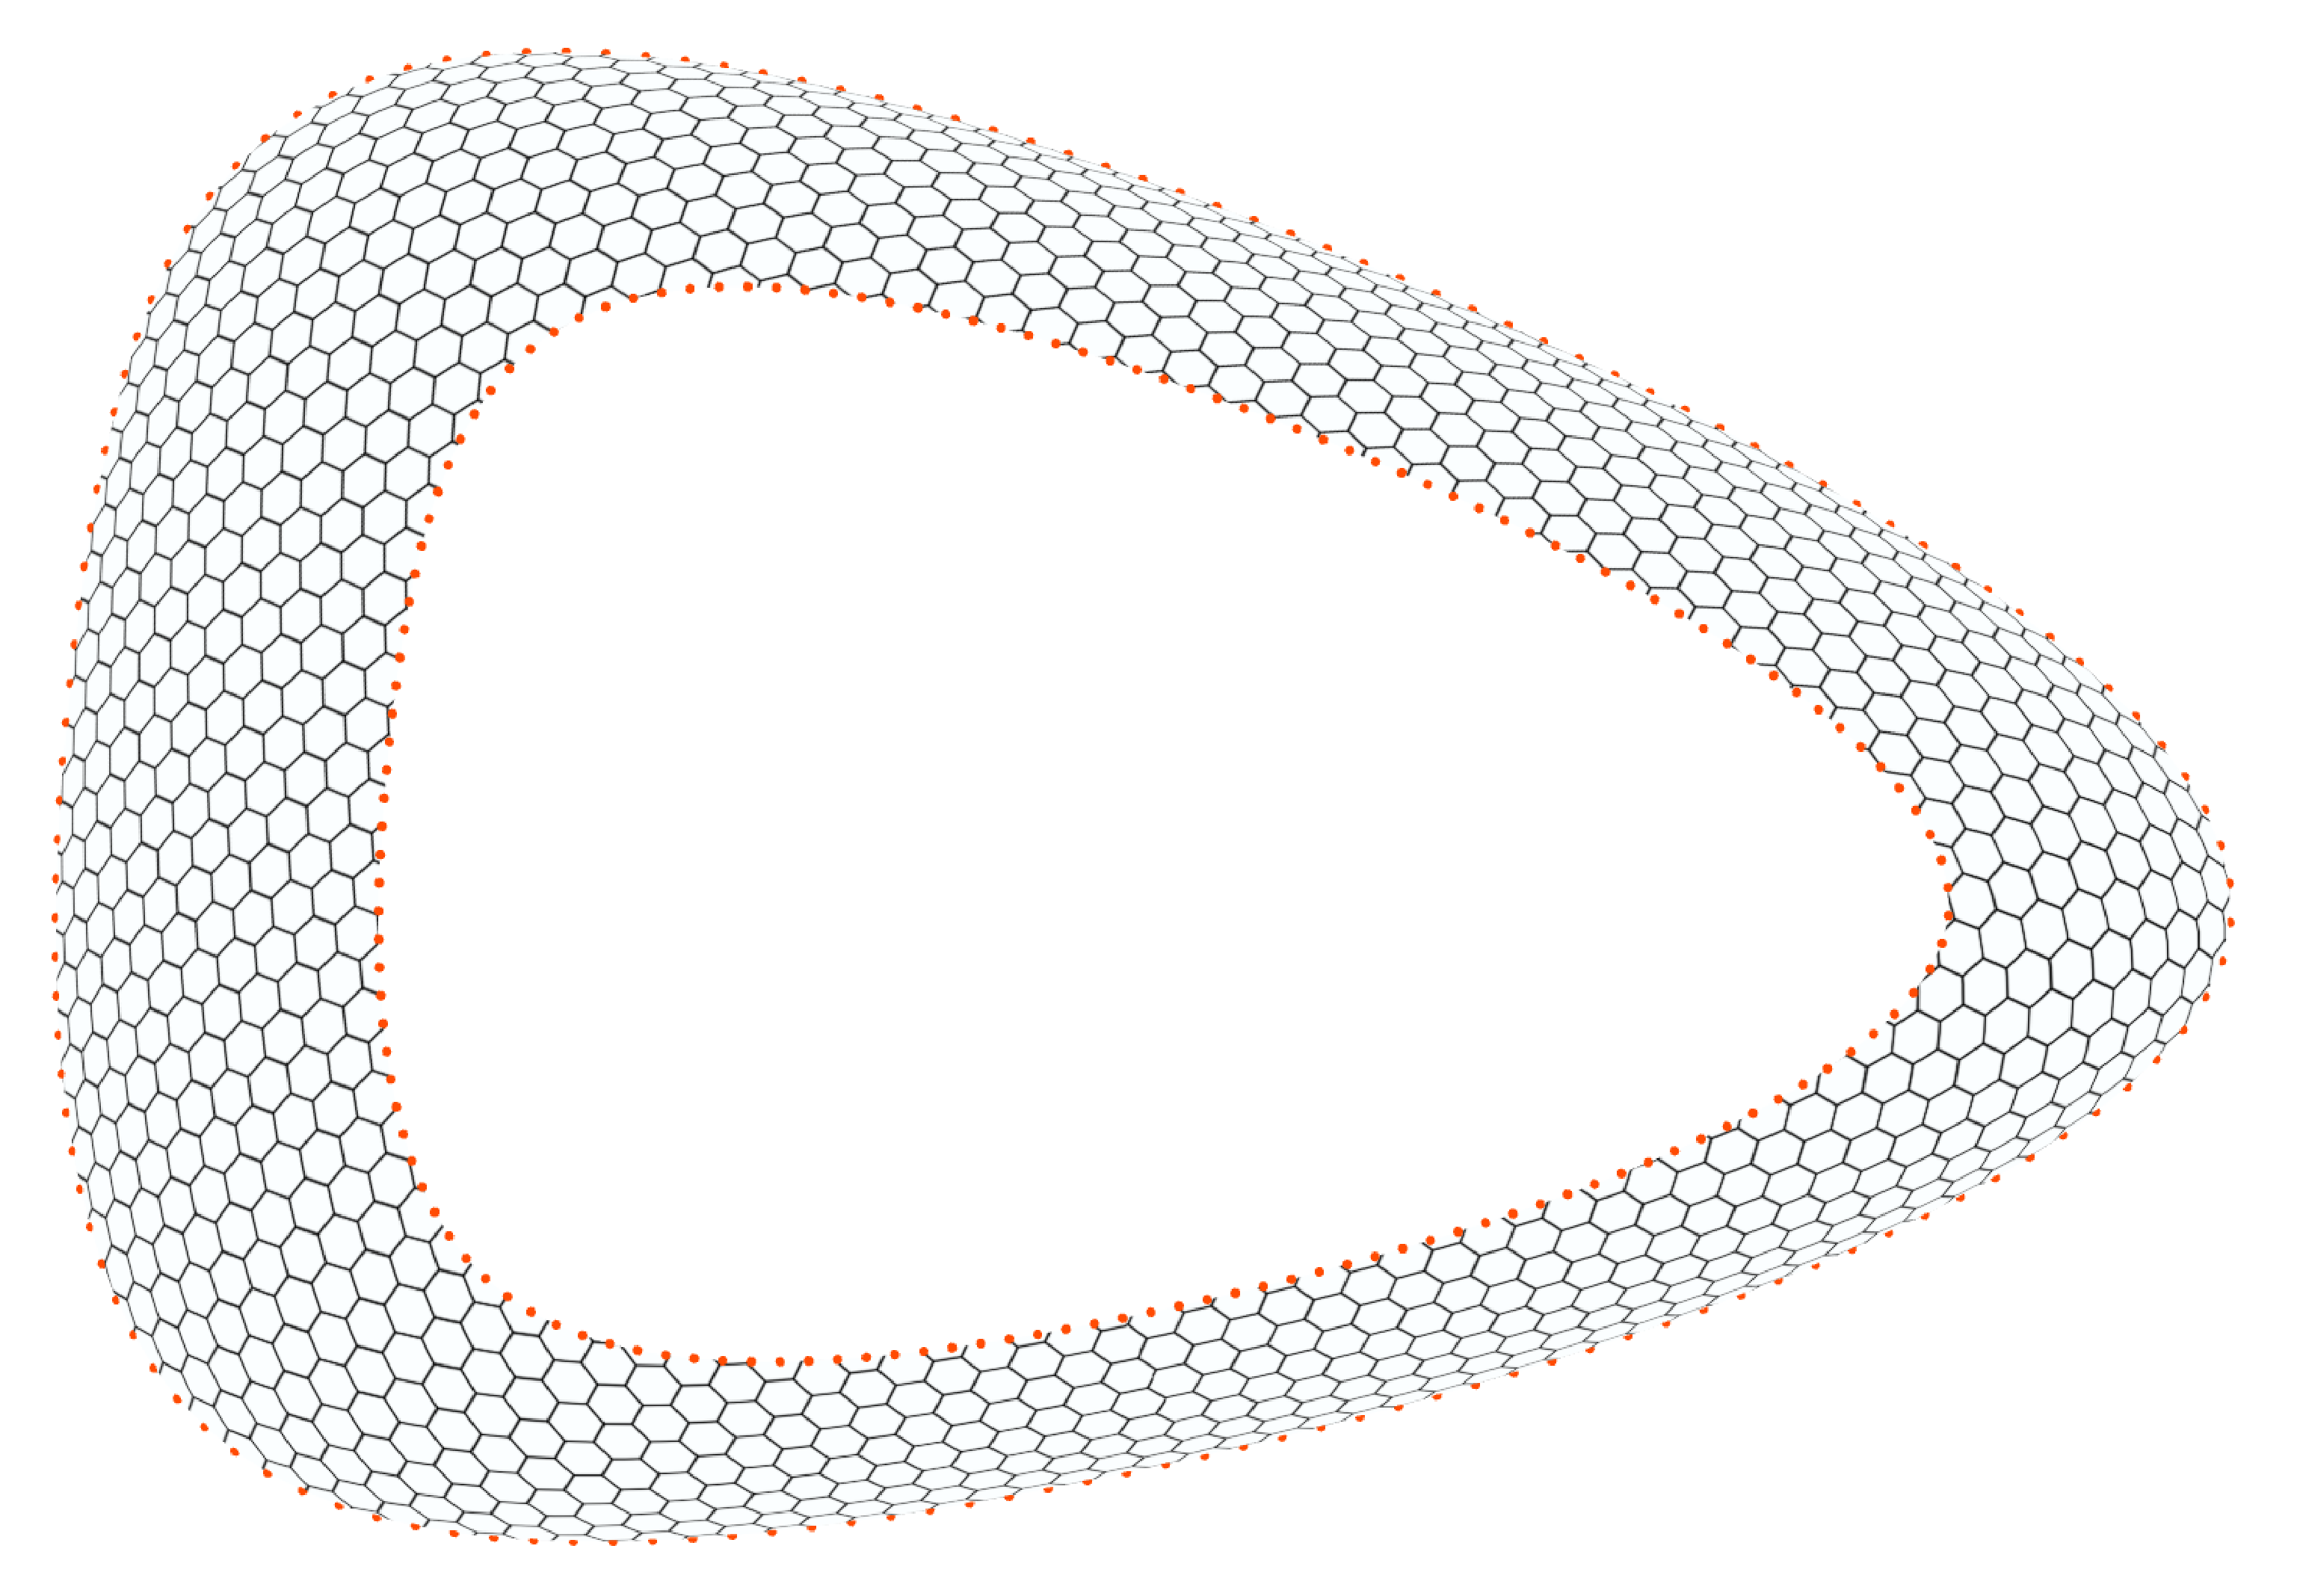
\includegraphics[width=6cm]{periodic/step02c_surface.pdf}		
            }
            \captionof{figure}{Map to cylinder with isometric boundary. Create a map with isometric boundary without cutting the mesh (left). Modify the resulting boundary angles to support a periodic pattern (middle). Periodic hexagonal pattern on the surface (right).}
\end{minipage}
\end{center}    

\item[(2)] We use the \emph{Cut and Glue Texture Domain} command and select \emph{Orthogonal to Boundary} to create a map to a rectangle (a) or a map to a polygonal region (b). In the isometric boundary case (c) we do not need a polygon as boundary curve.
\item[(3)] Select a predefined texture for quadrilateral, triangle, or hexagonal mesh preview from the \emph{Content Appearance$\to$Texture} panel. Adjust the texture scale to a reasonable value. In the isometric case (c) we close the period with the \emph{Texture Transformation} user interface manually. For cases (a) and (b), periods will be closed automatically by the remeshing algorithm.

\begin{center}
\begin{minipage}{0.9\linewidth}
            \centering
            \resizebox{\linewidth}{!}{
            	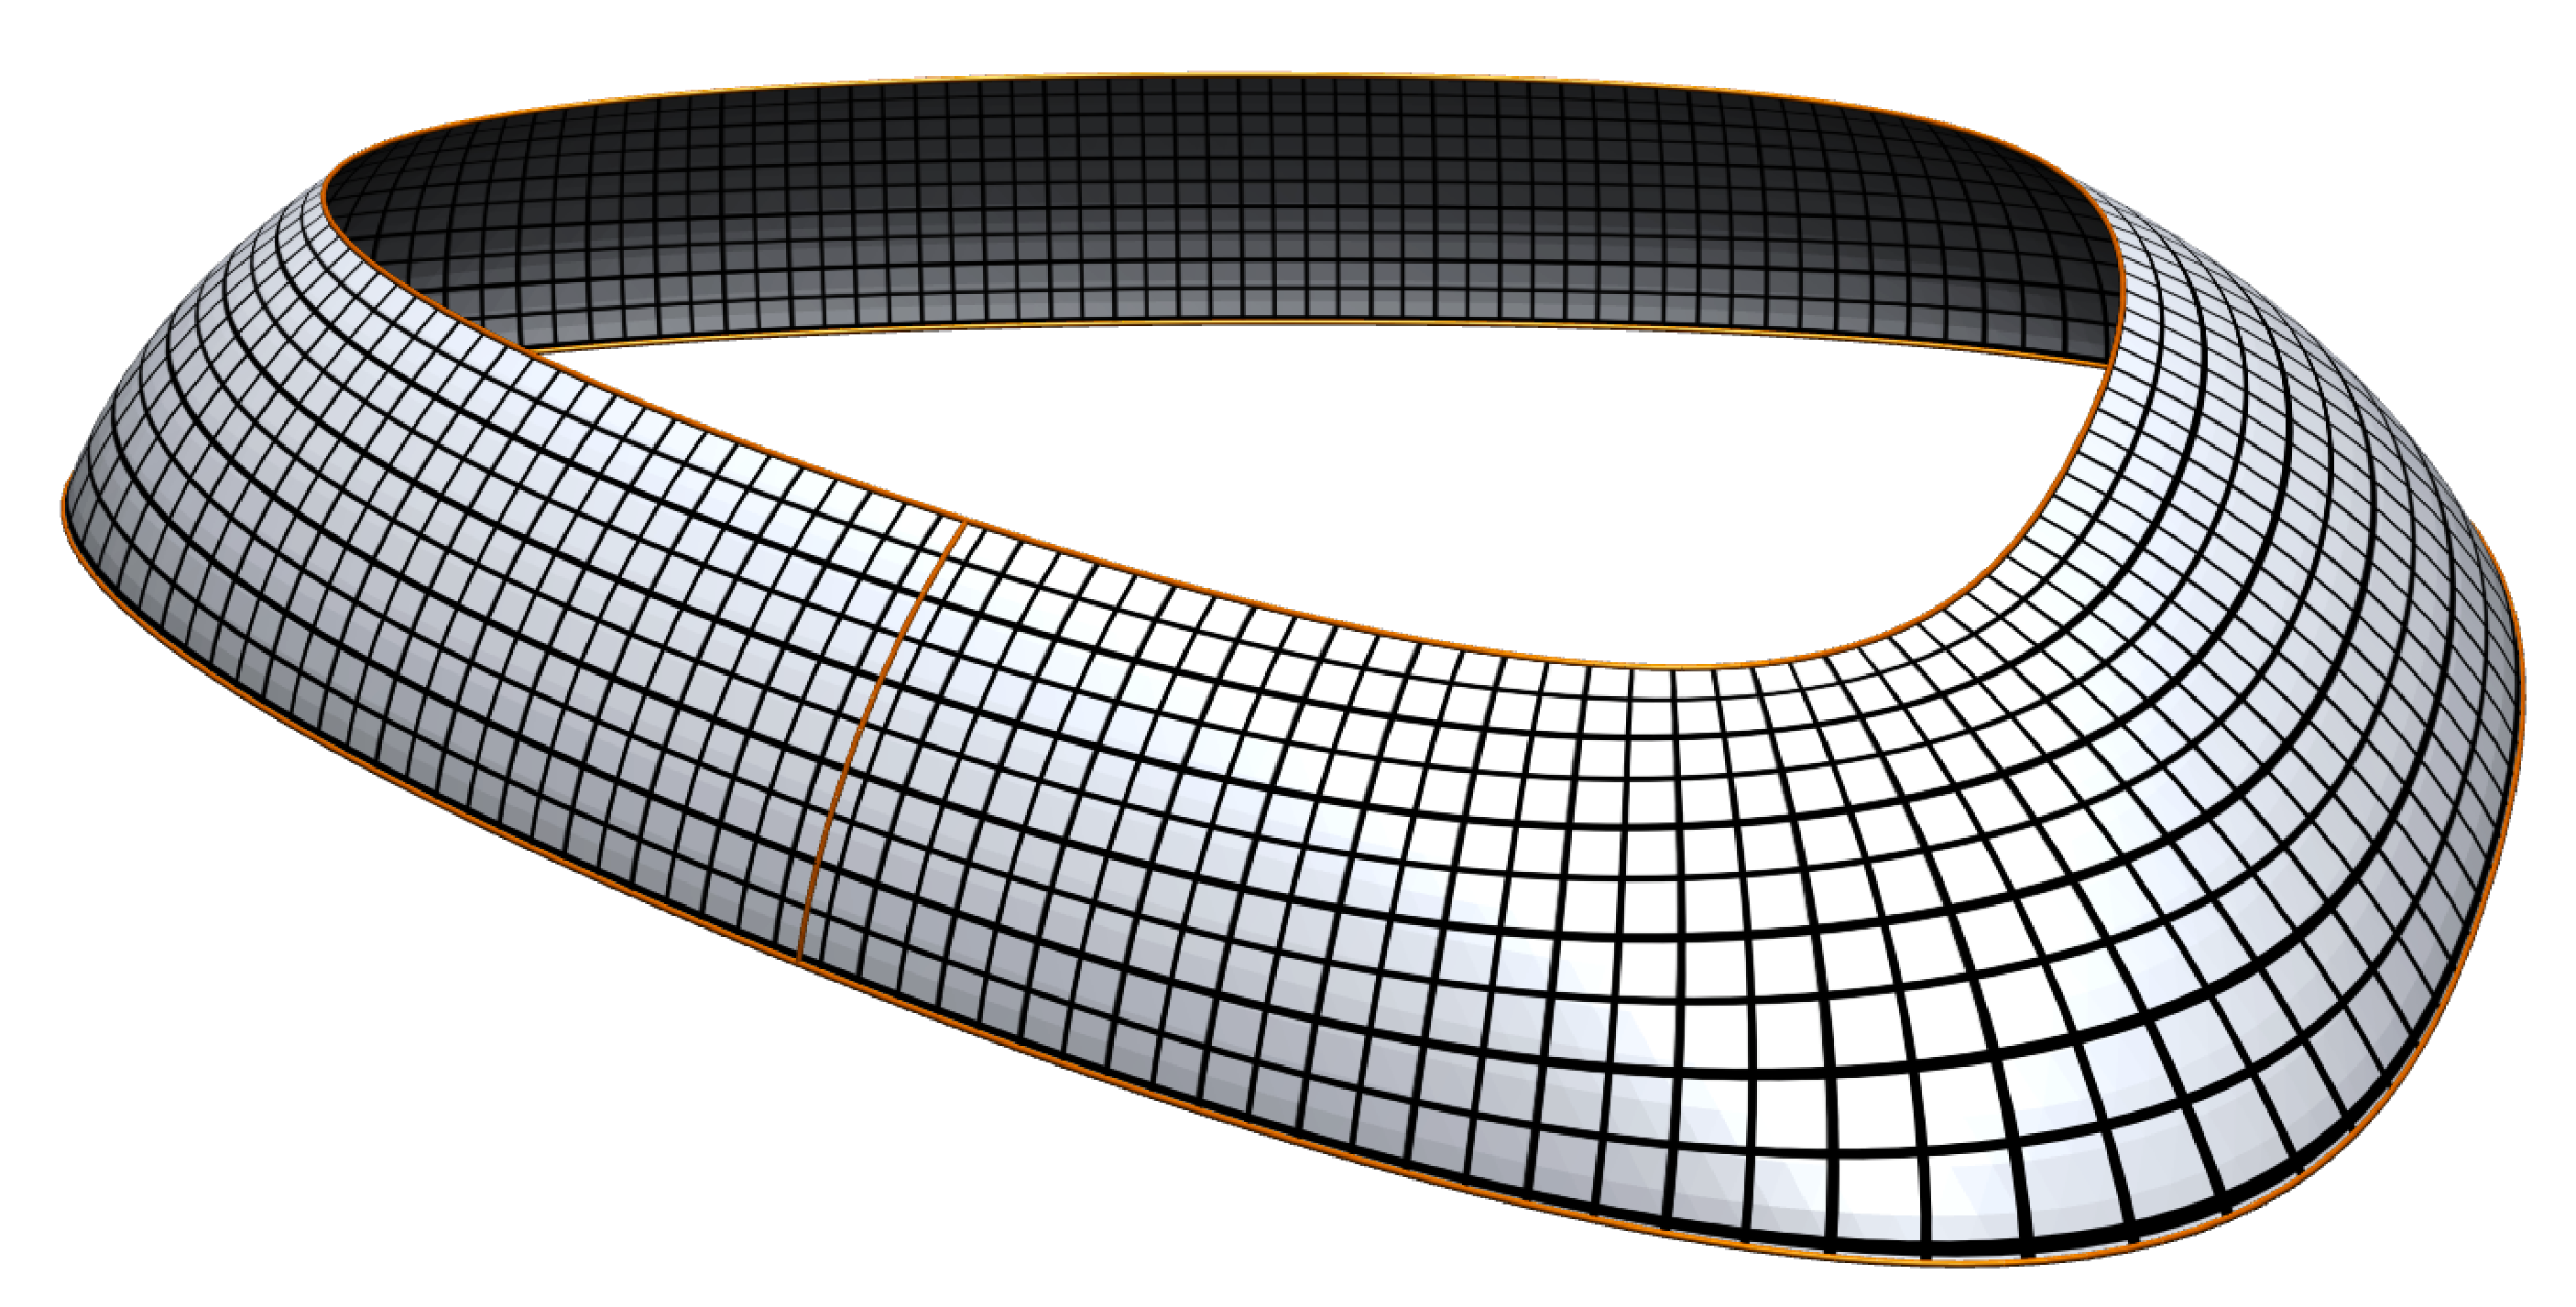
\includegraphics[width=5cm]{periodic/step03_quads.pdf}
            	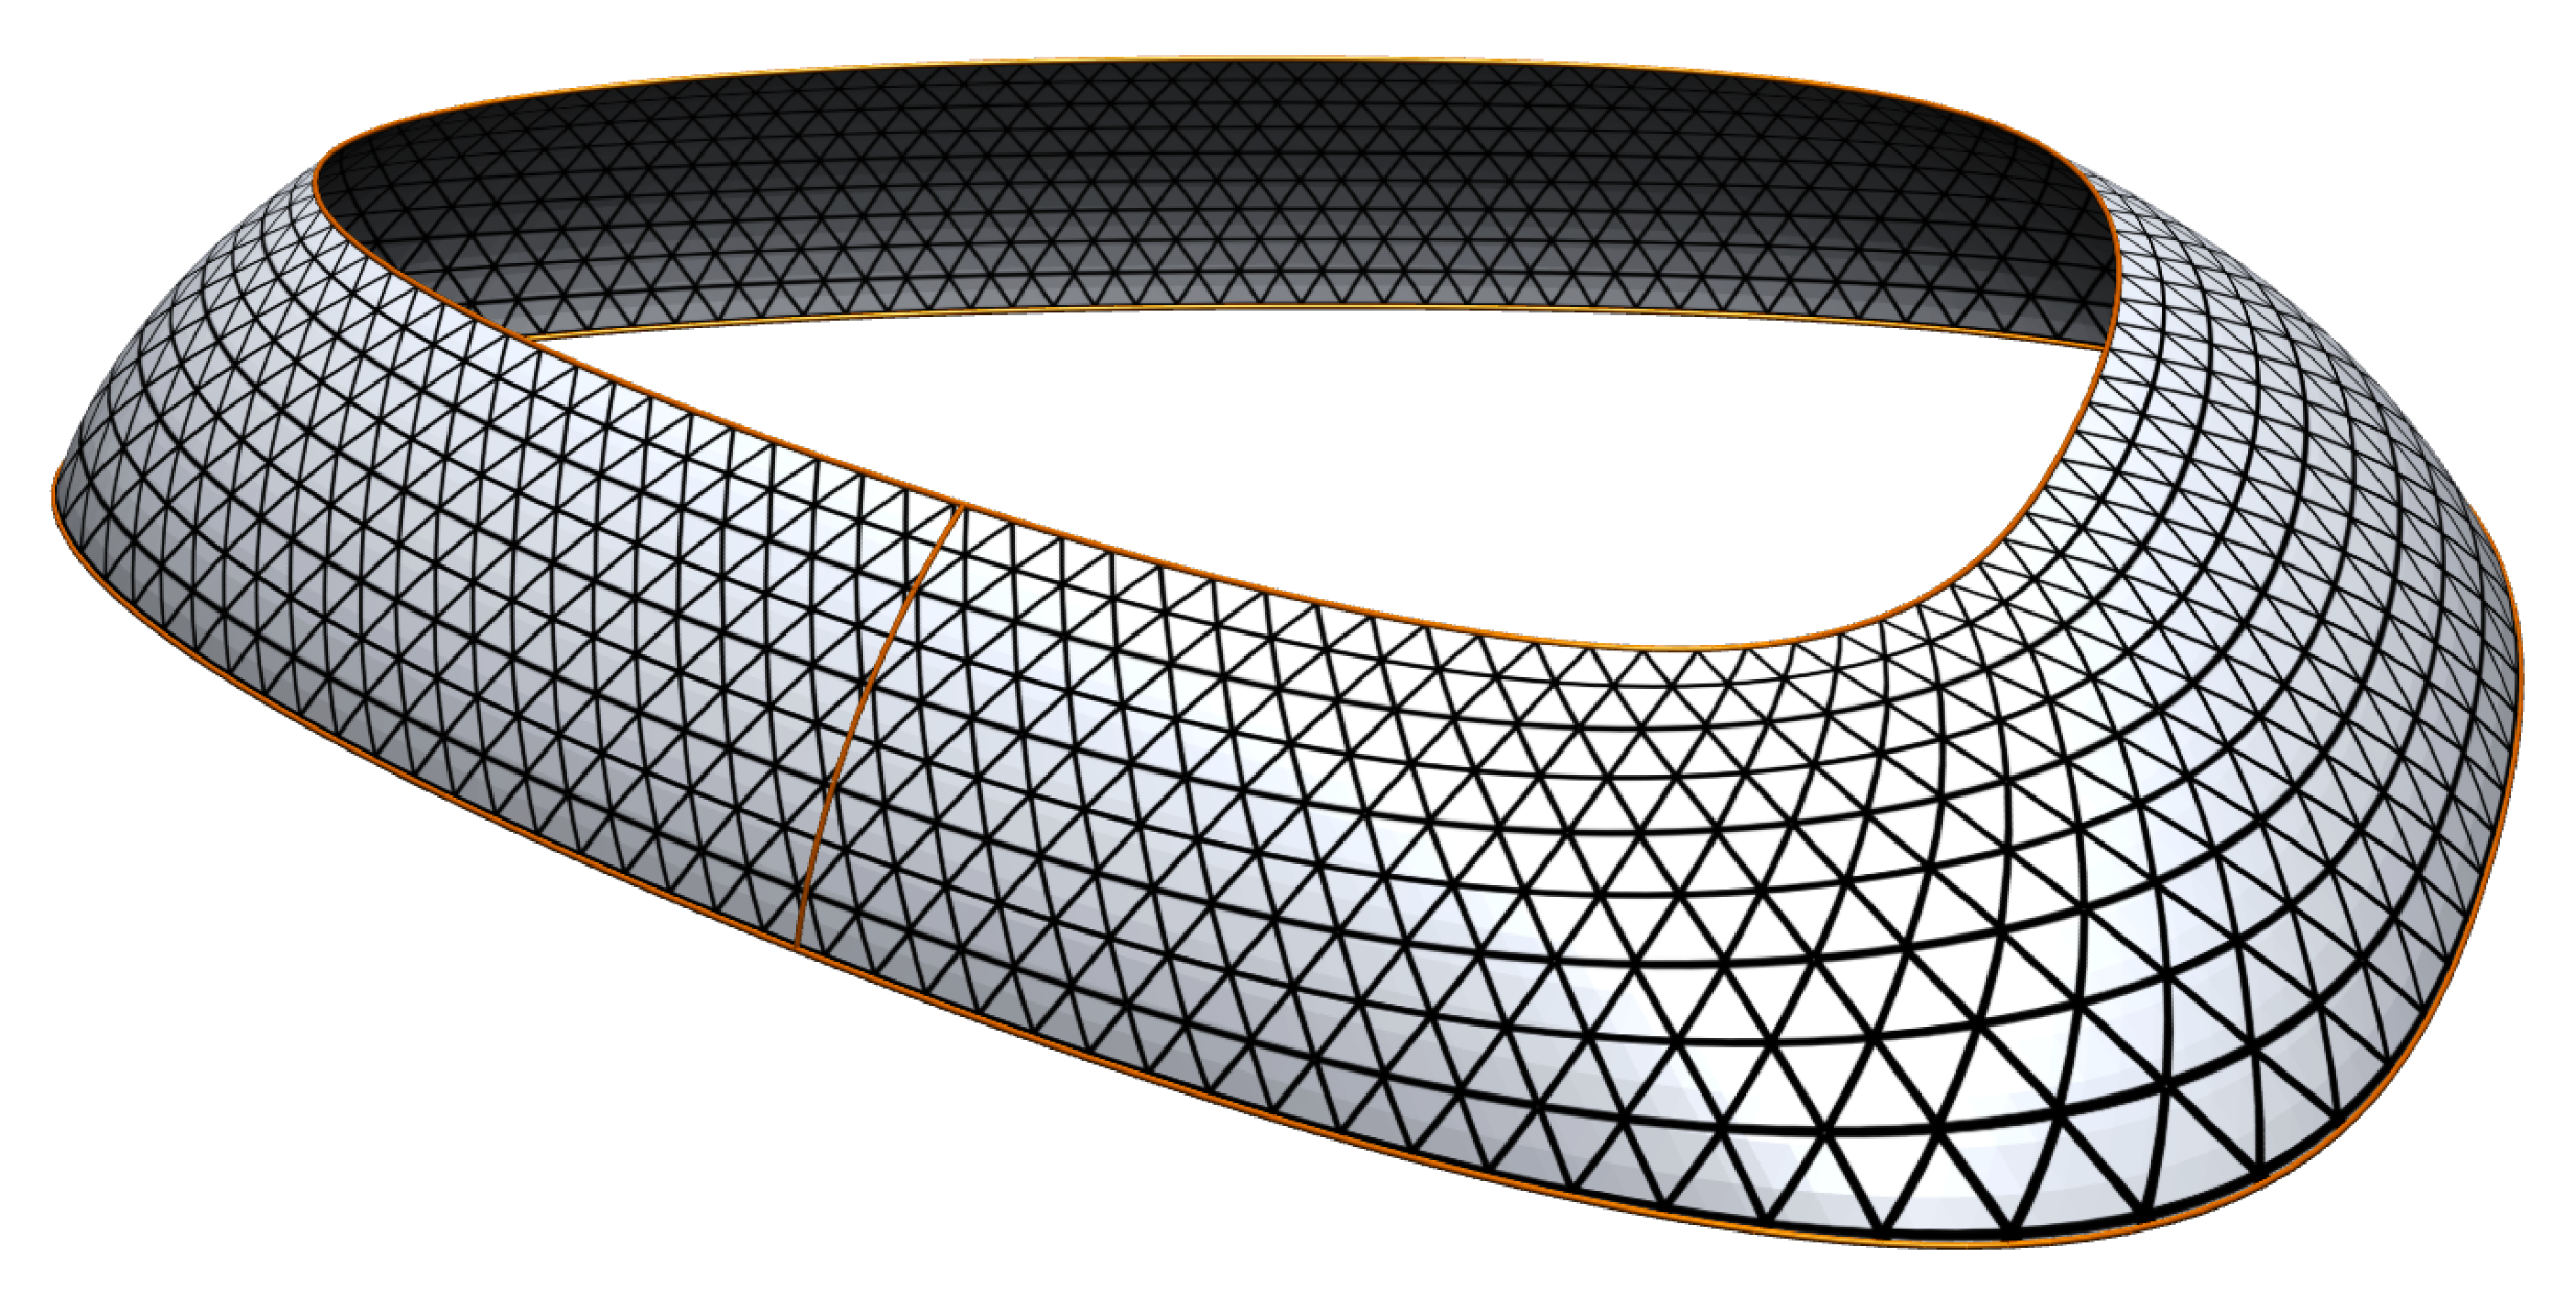
\includegraphics[width=5cm]{periodic/step03_triangles.pdf}	
            	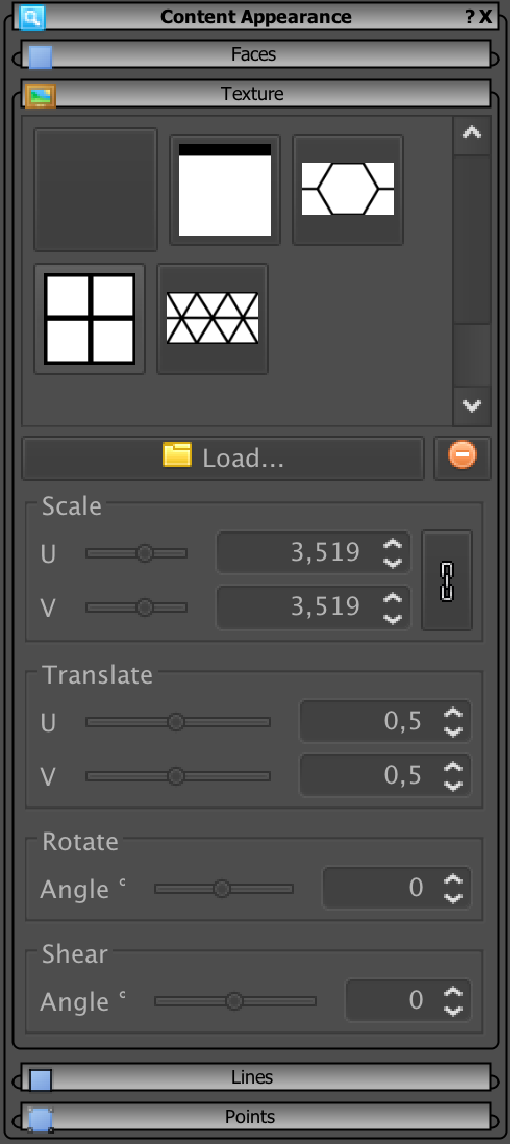
\includegraphics[width=1.5cm]{periodic/step03_ui.pdf}	
            }
            \captionof{figure}{Pattern preview.}
\end{minipage}
\end{center}    

\item[(4)] Perform remeshing in cases (a) and (b) either for \emph{Boundary Aligned Triangles} or \emph{Boundary Aligned Quads} using the \emph{Surface Remeshing} panel. For non-boundary-aligned parameterization (c) we use the \emph{Quads With Singularities/Triangles With Singularities} remeshing mode.\\

\begin{center}
\begin{minipage}{0.9\linewidth}
            \centering
            \resizebox{\linewidth}{!}{
            	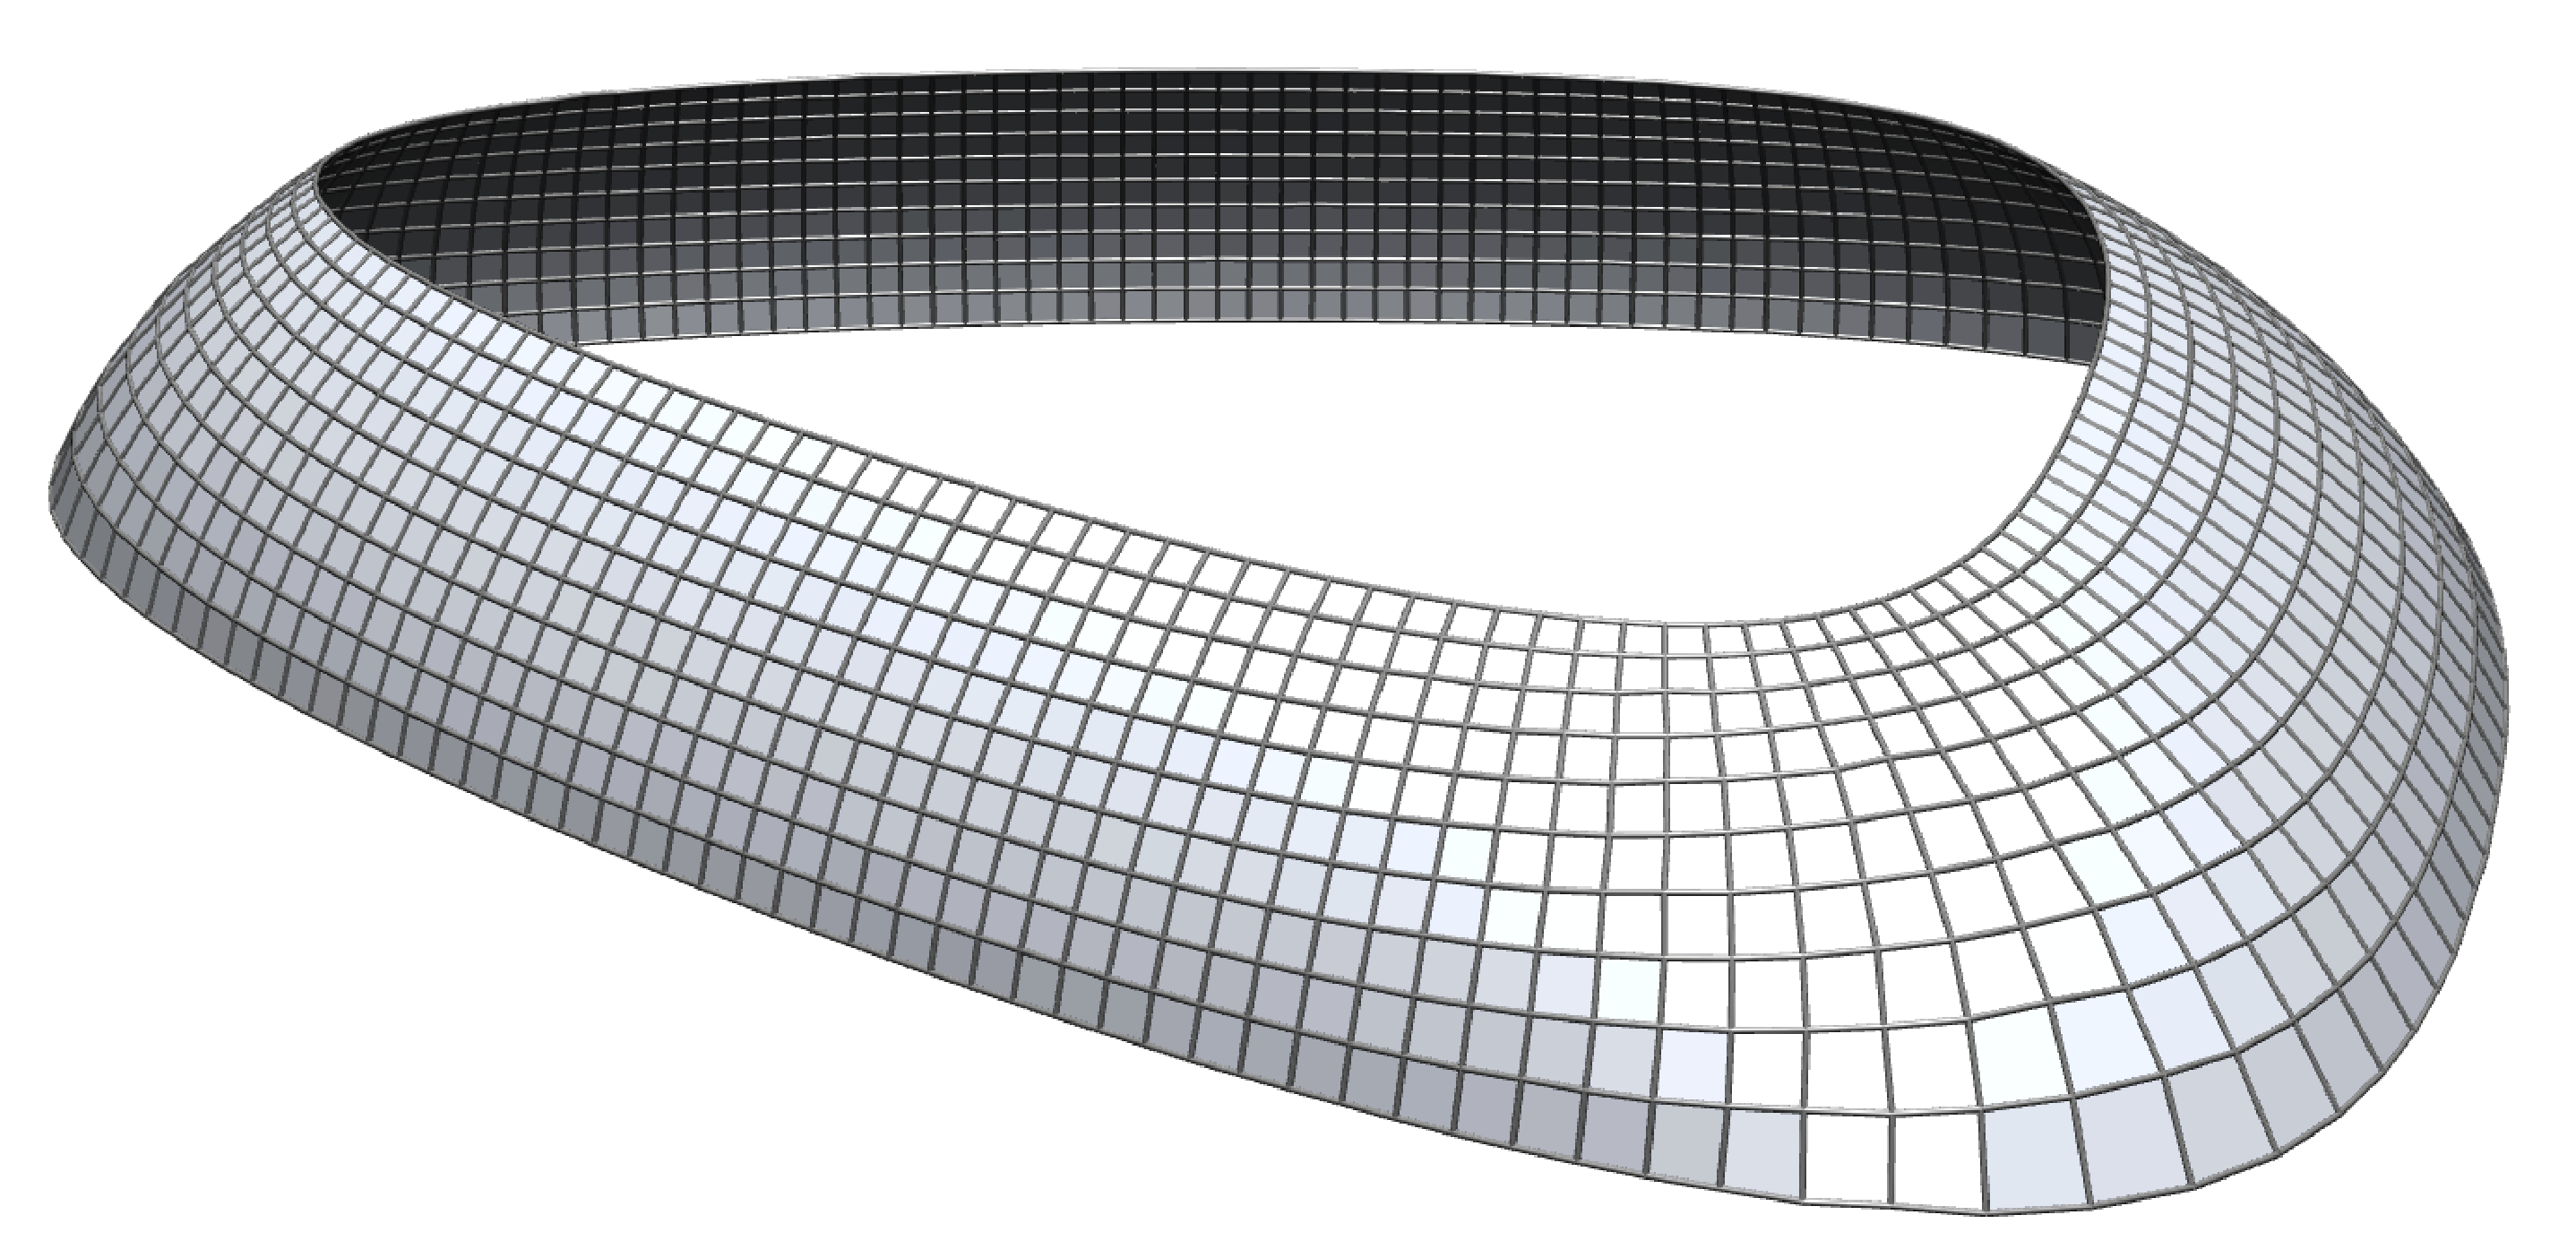
\includegraphics[width=5cm]{periodic/step04_quads_surface.pdf}
            	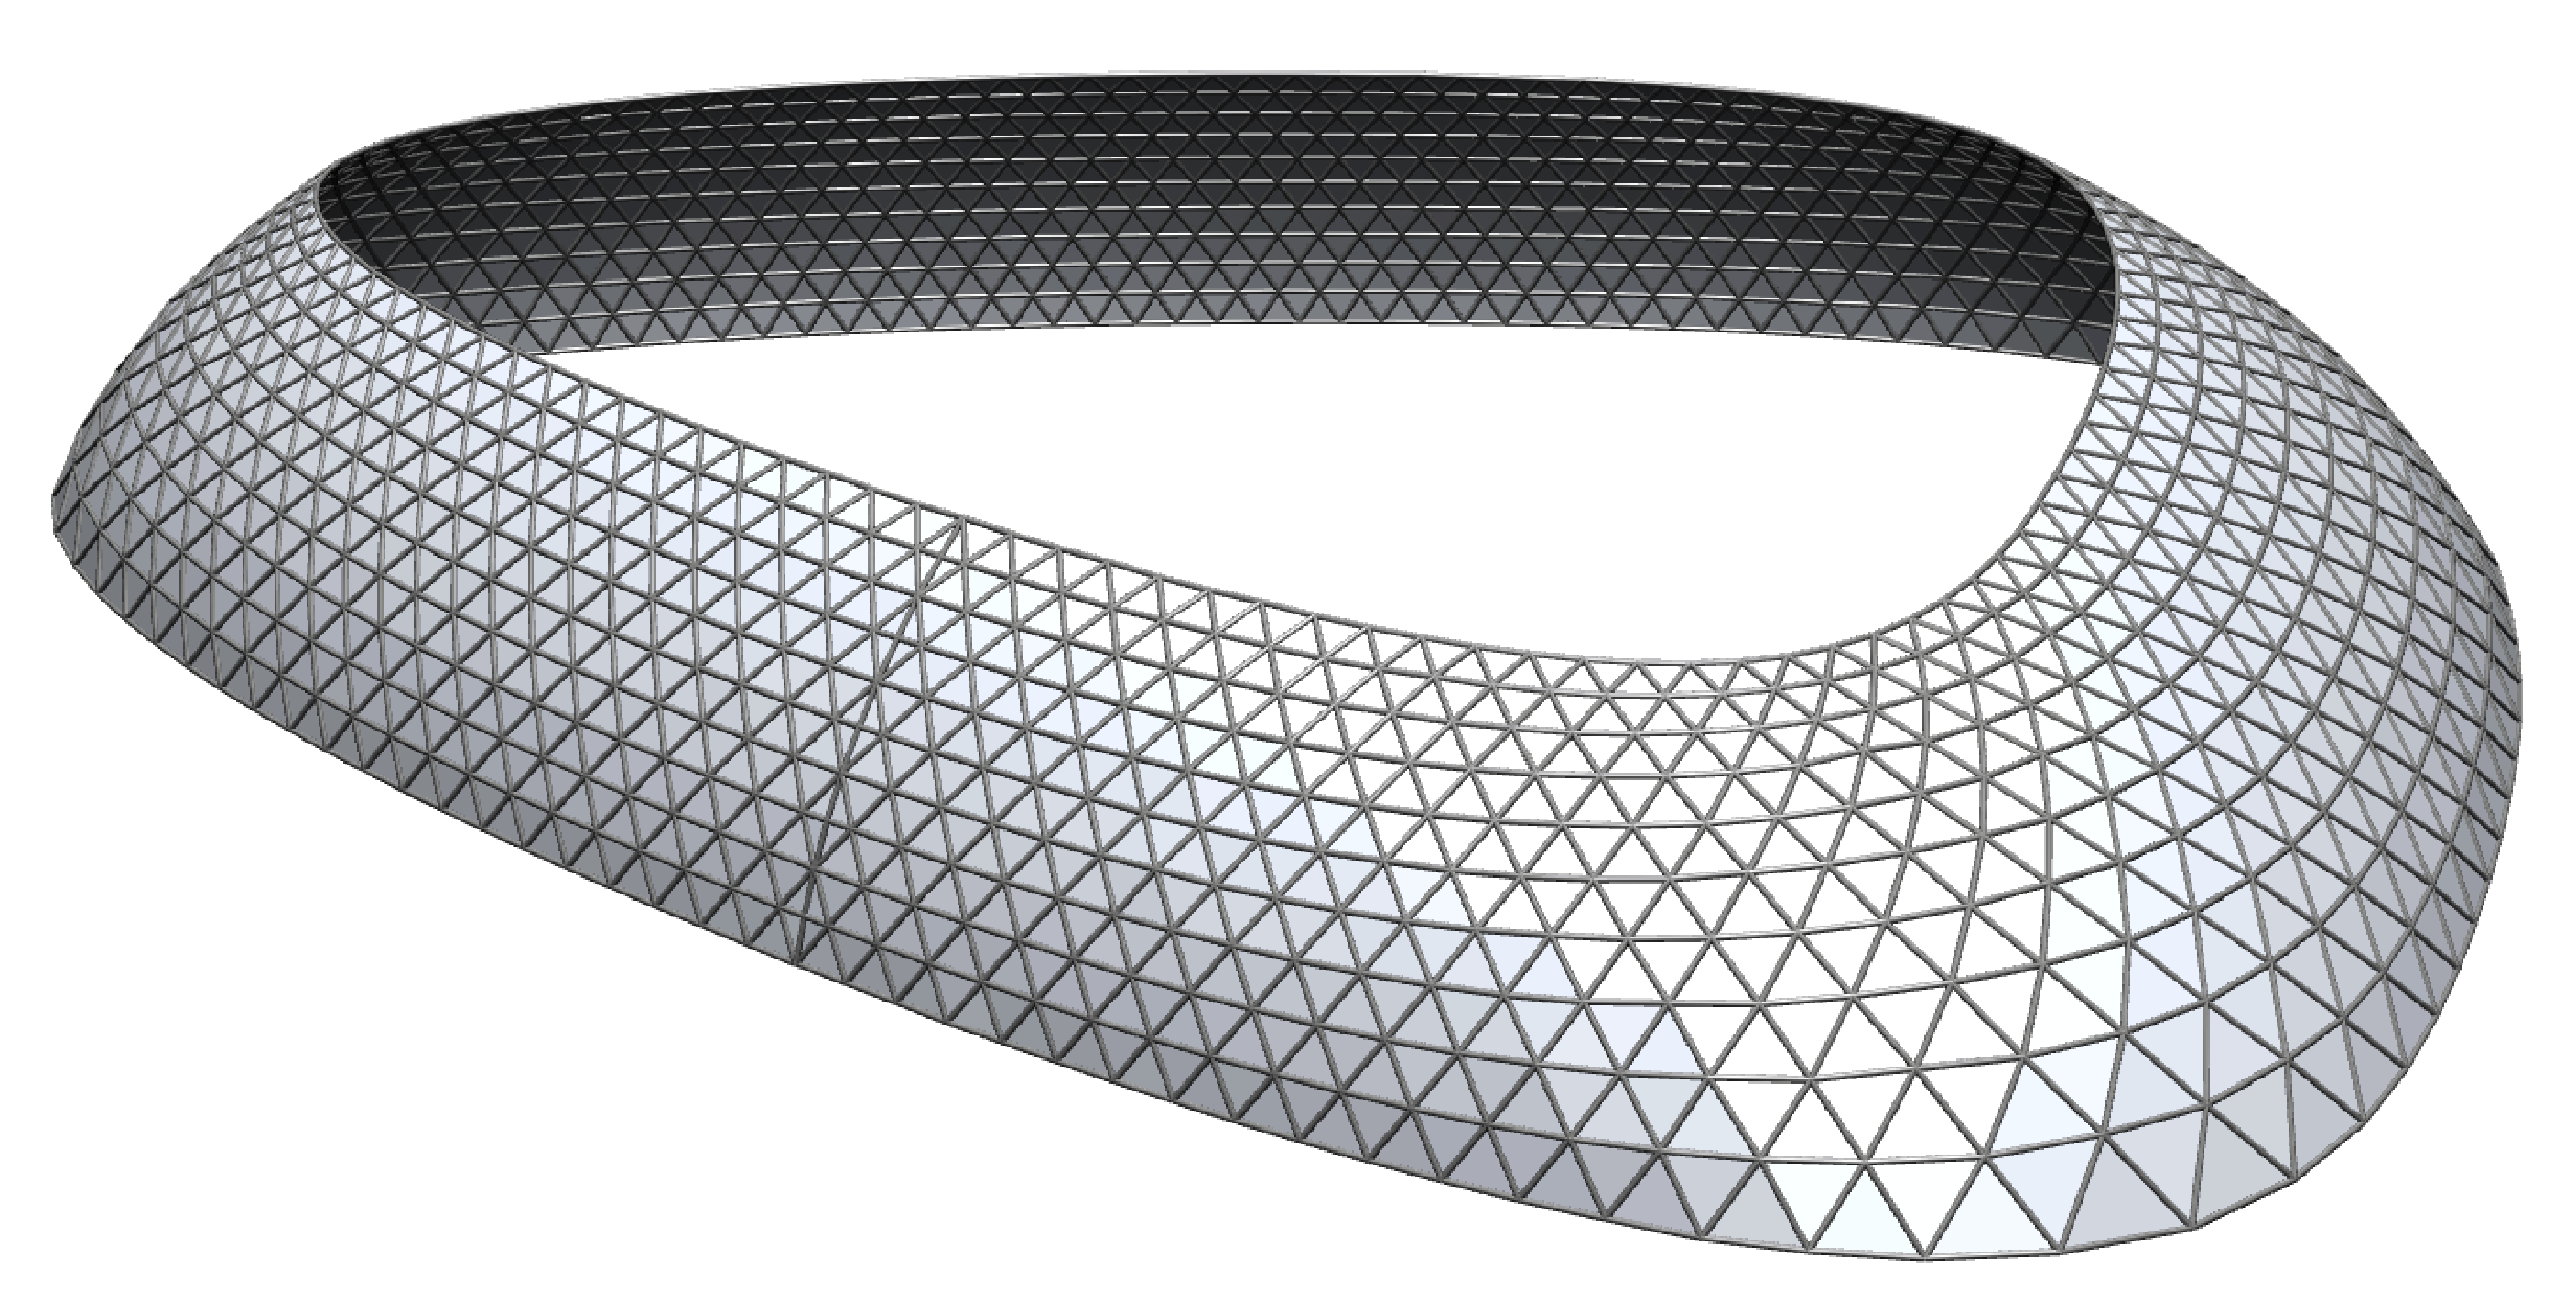
\includegraphics[width=5cm]{periodic/step04_triangles_surface.pdf}	
            	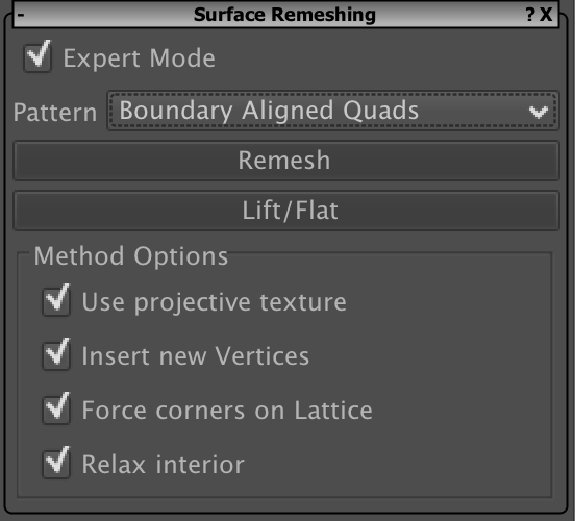
\includegraphics[width=2cm]{periodic/step04_ui.pdf}	
            }
            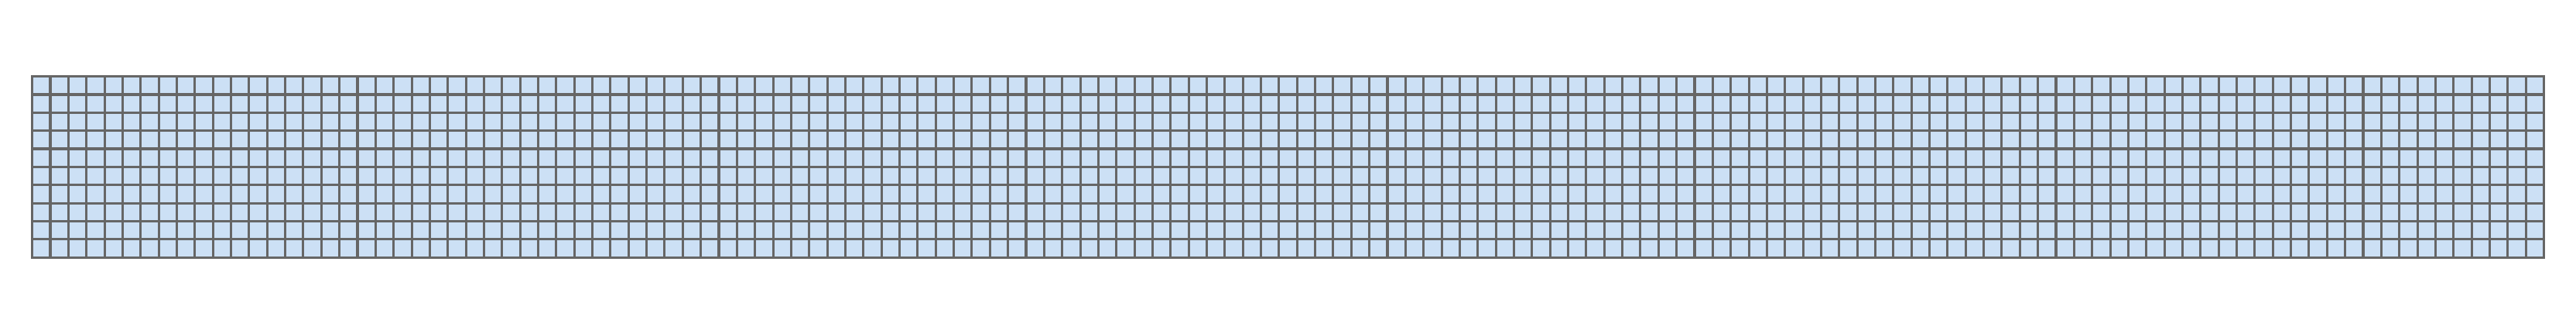
\includegraphics[width=\linewidth]{periodic/step04_quads_map.pdf}
            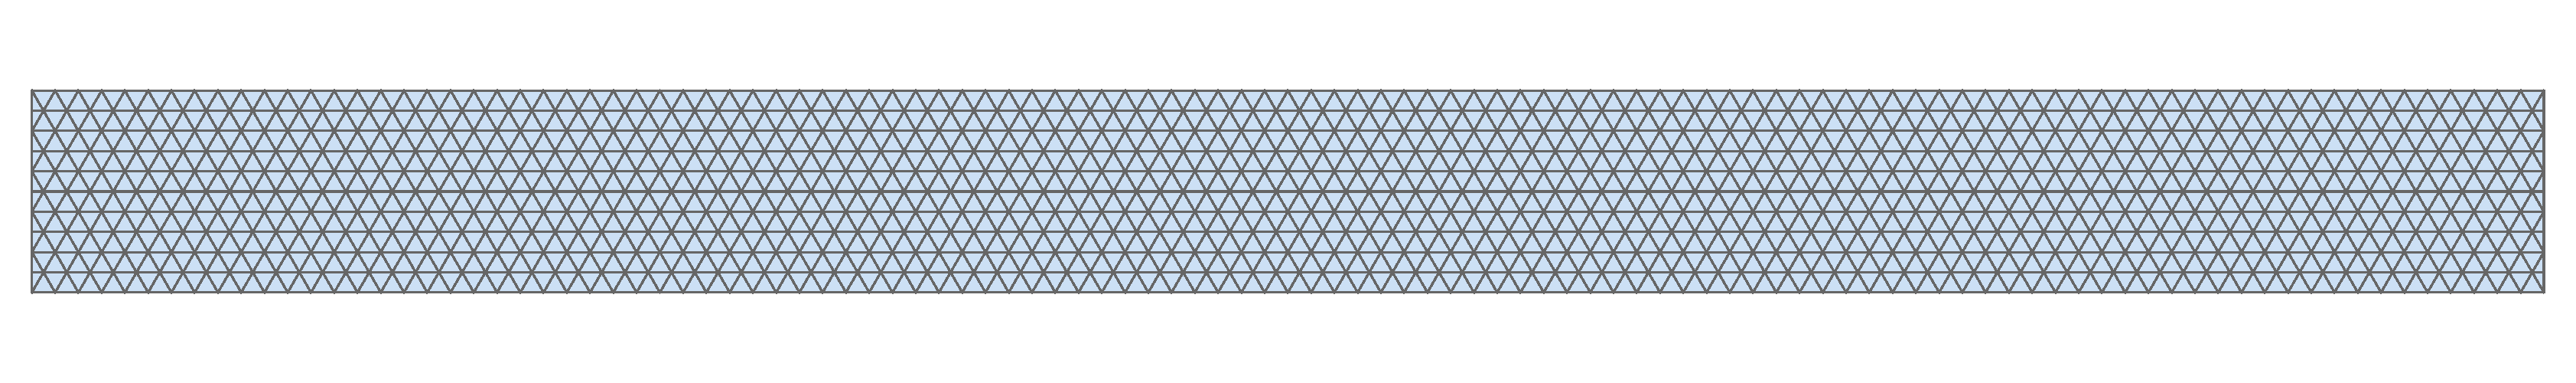
\includegraphics[width=\linewidth]{periodic/step04_triangles_map.pdf}
            \captionof{figure}{New mesh and domain.}
\end{minipage}
\end{center}    

\item[(5)] We create a watertight mesh using the \emph{Watertight Mesh Generator} and remove extra edges and vertices. In the isometric case (c) we use a combination of \emph{Topology$\to$Stitch} and \emph{Topology$\to$Stitch Cut Path} to remove the cut path from the mesh.
\item[(6)] For hexagonal mesh creation we select from the periodic triangle mesh all centers of hexagons using the \emph{Selection$\to$Lattice} command. The \emph{Remove Vertex and Fill} command then creates a periodic hexagonal mesh.
\begin{center}
\begin{minipage}{0.9\linewidth}
            \centering
            \resizebox{\linewidth}{!}{
            	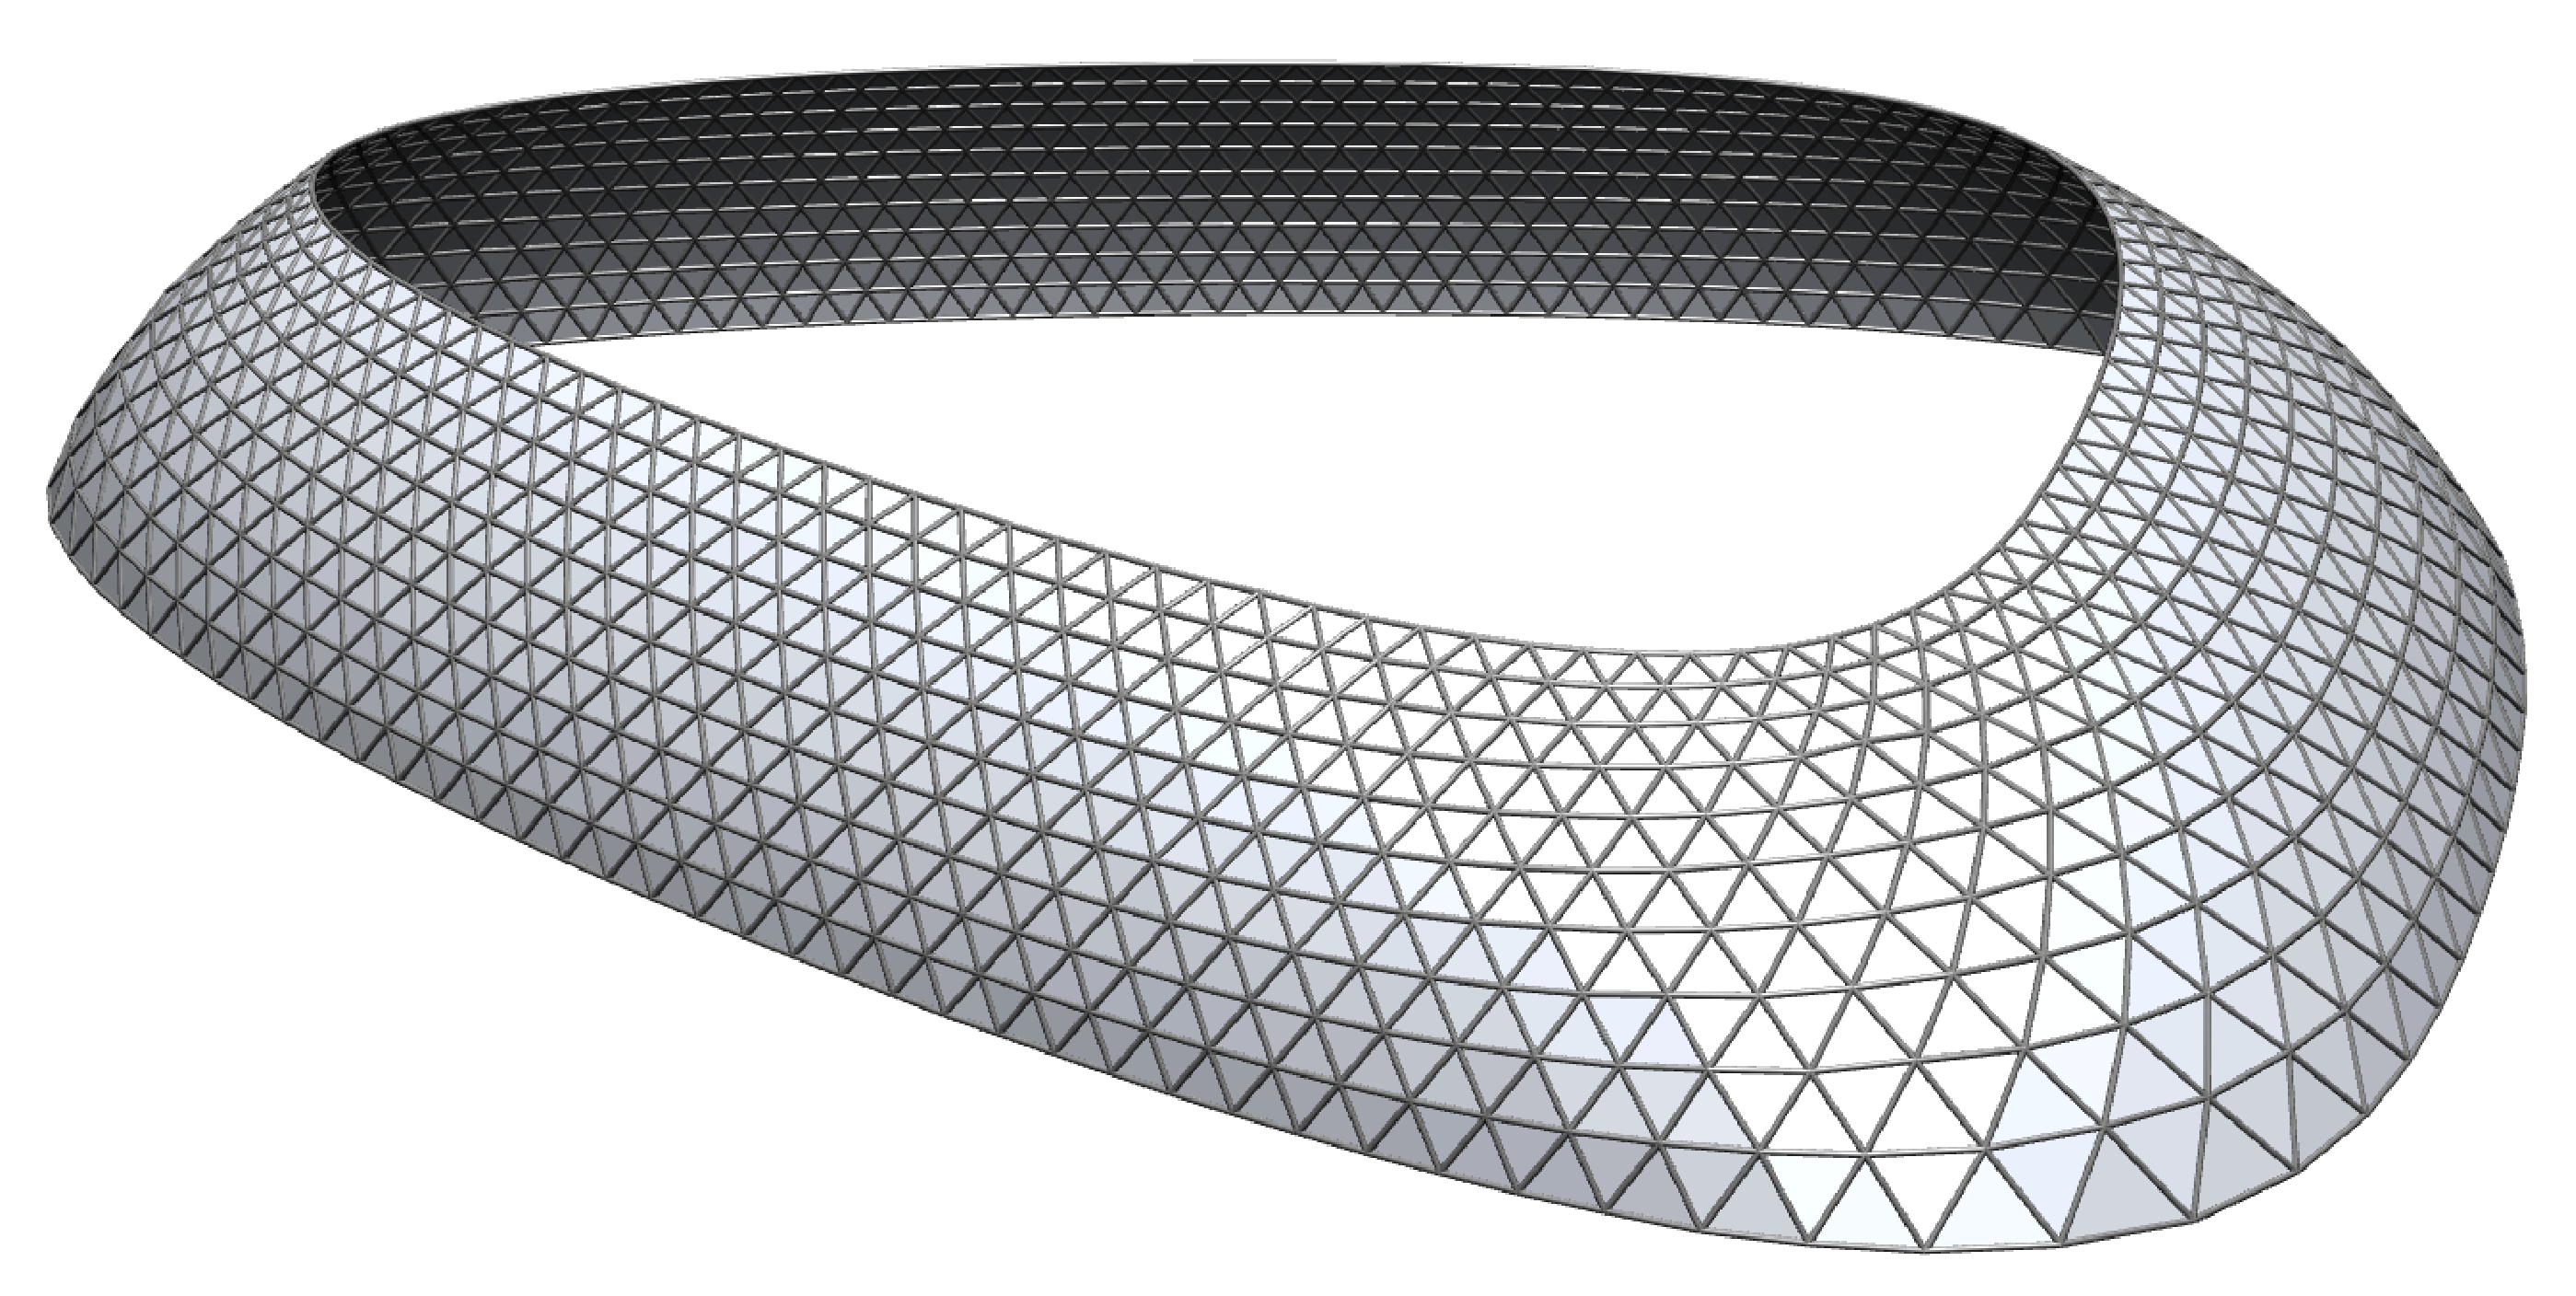
\includegraphics{periodic/step05.pdf}
            	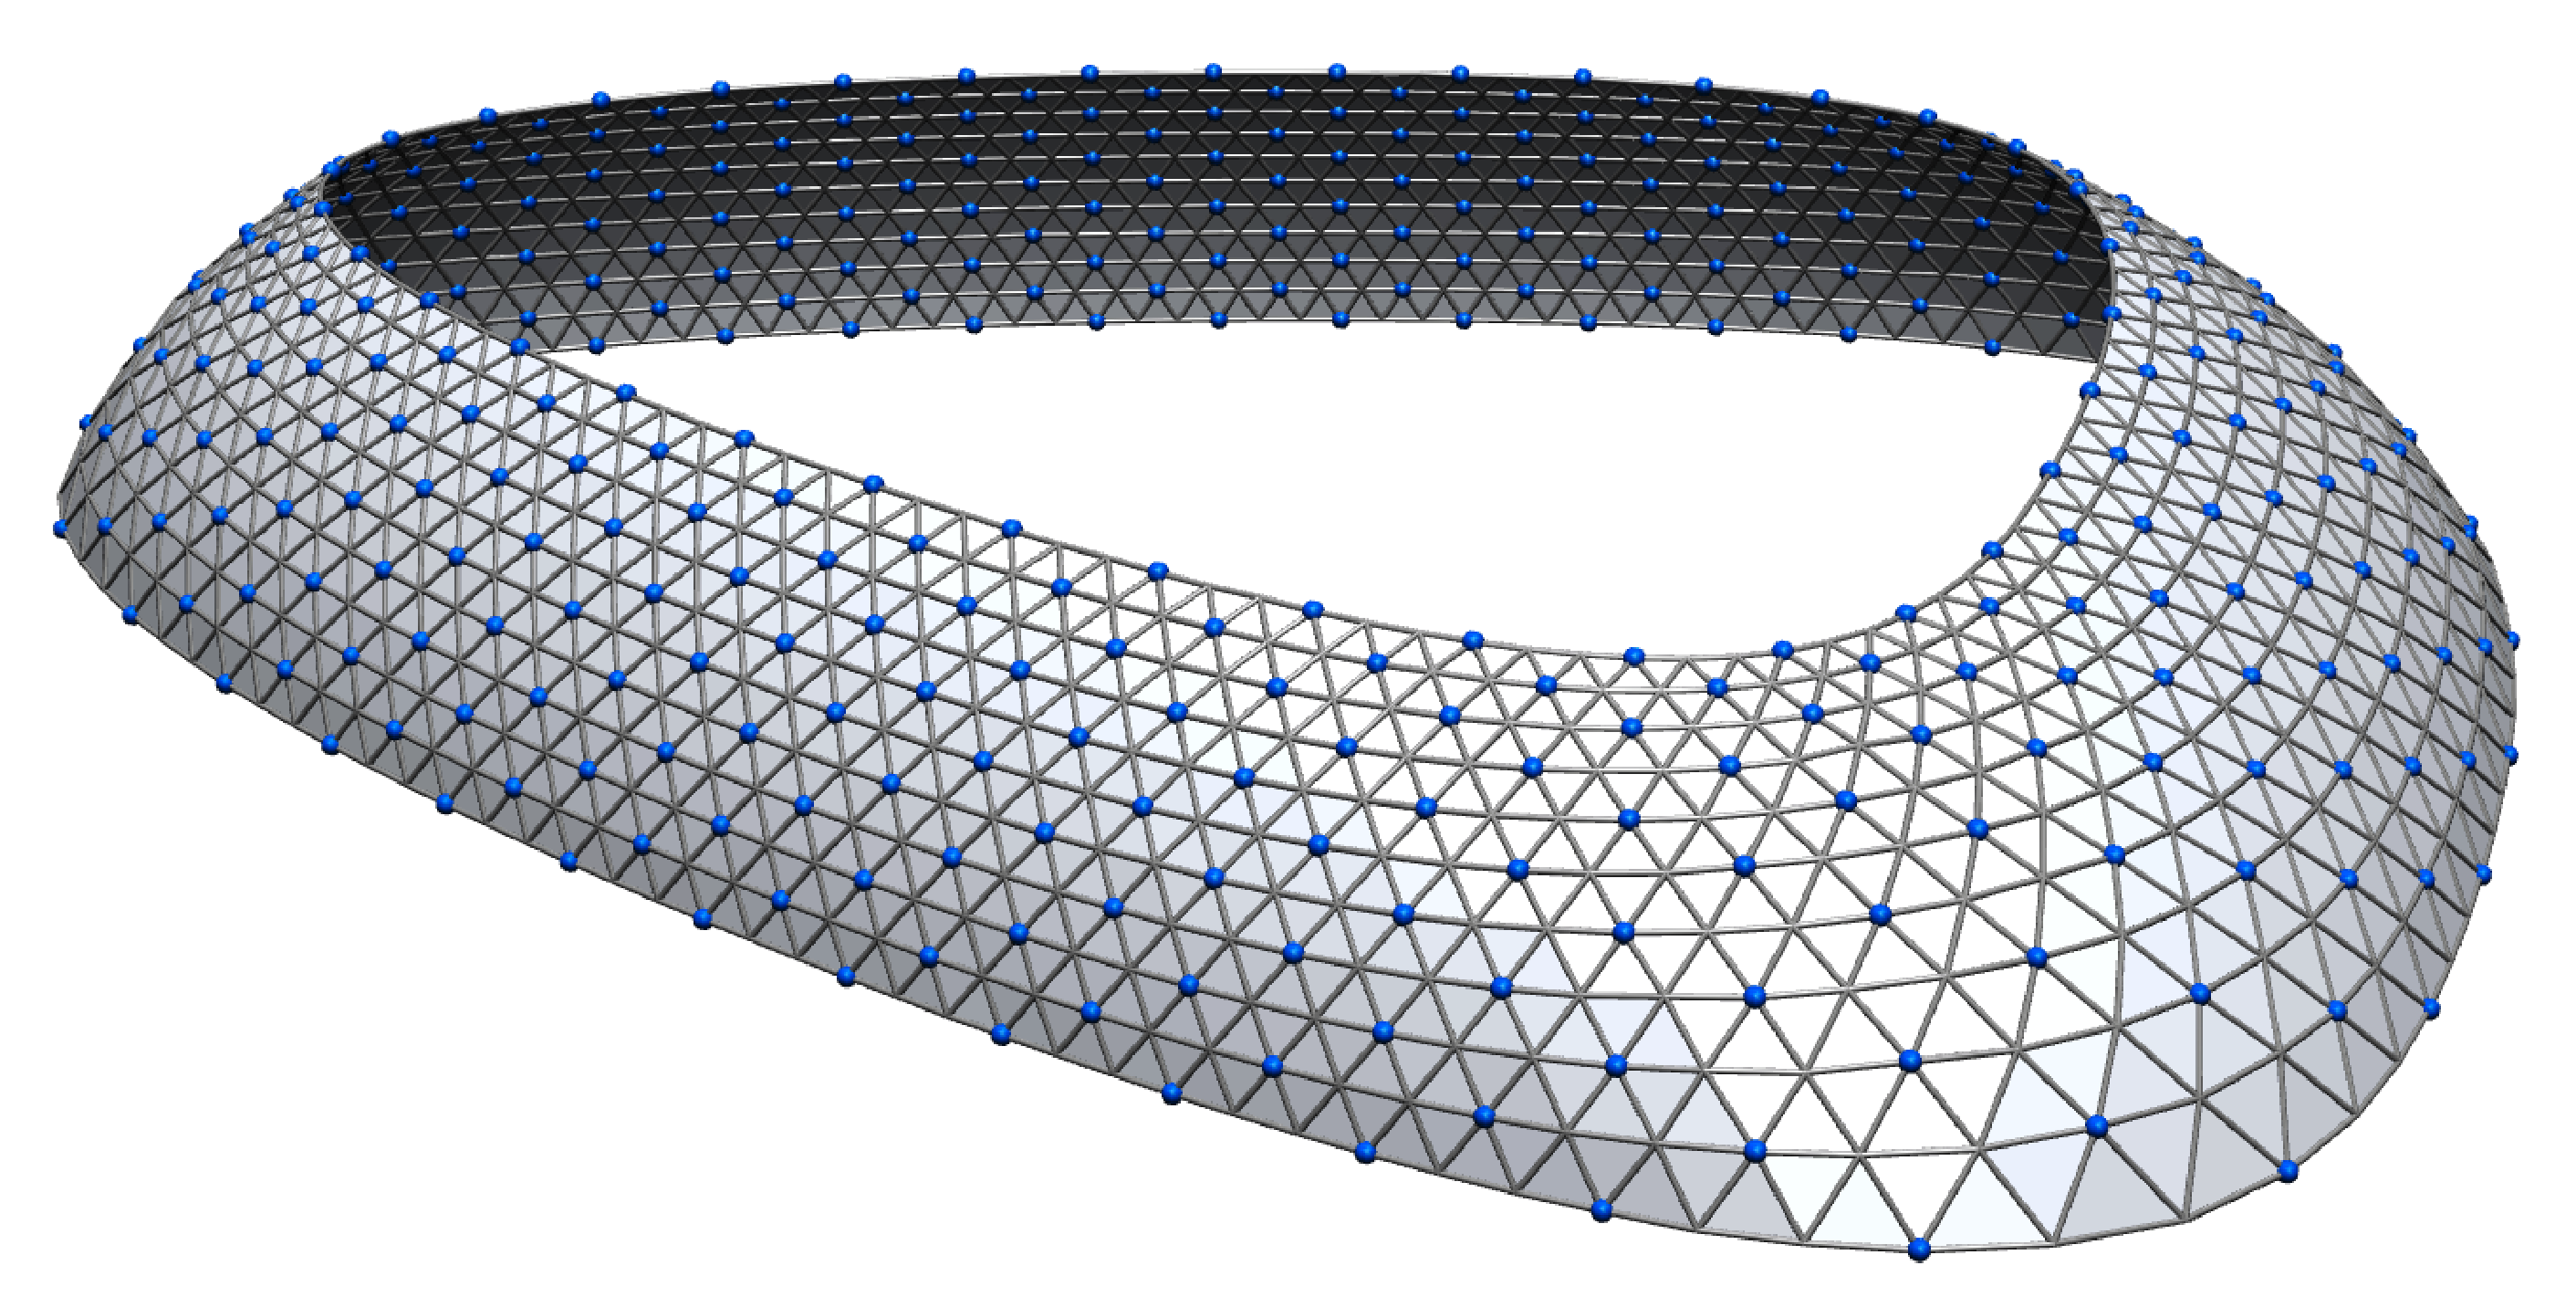
\includegraphics{periodic/step06.pdf}
            	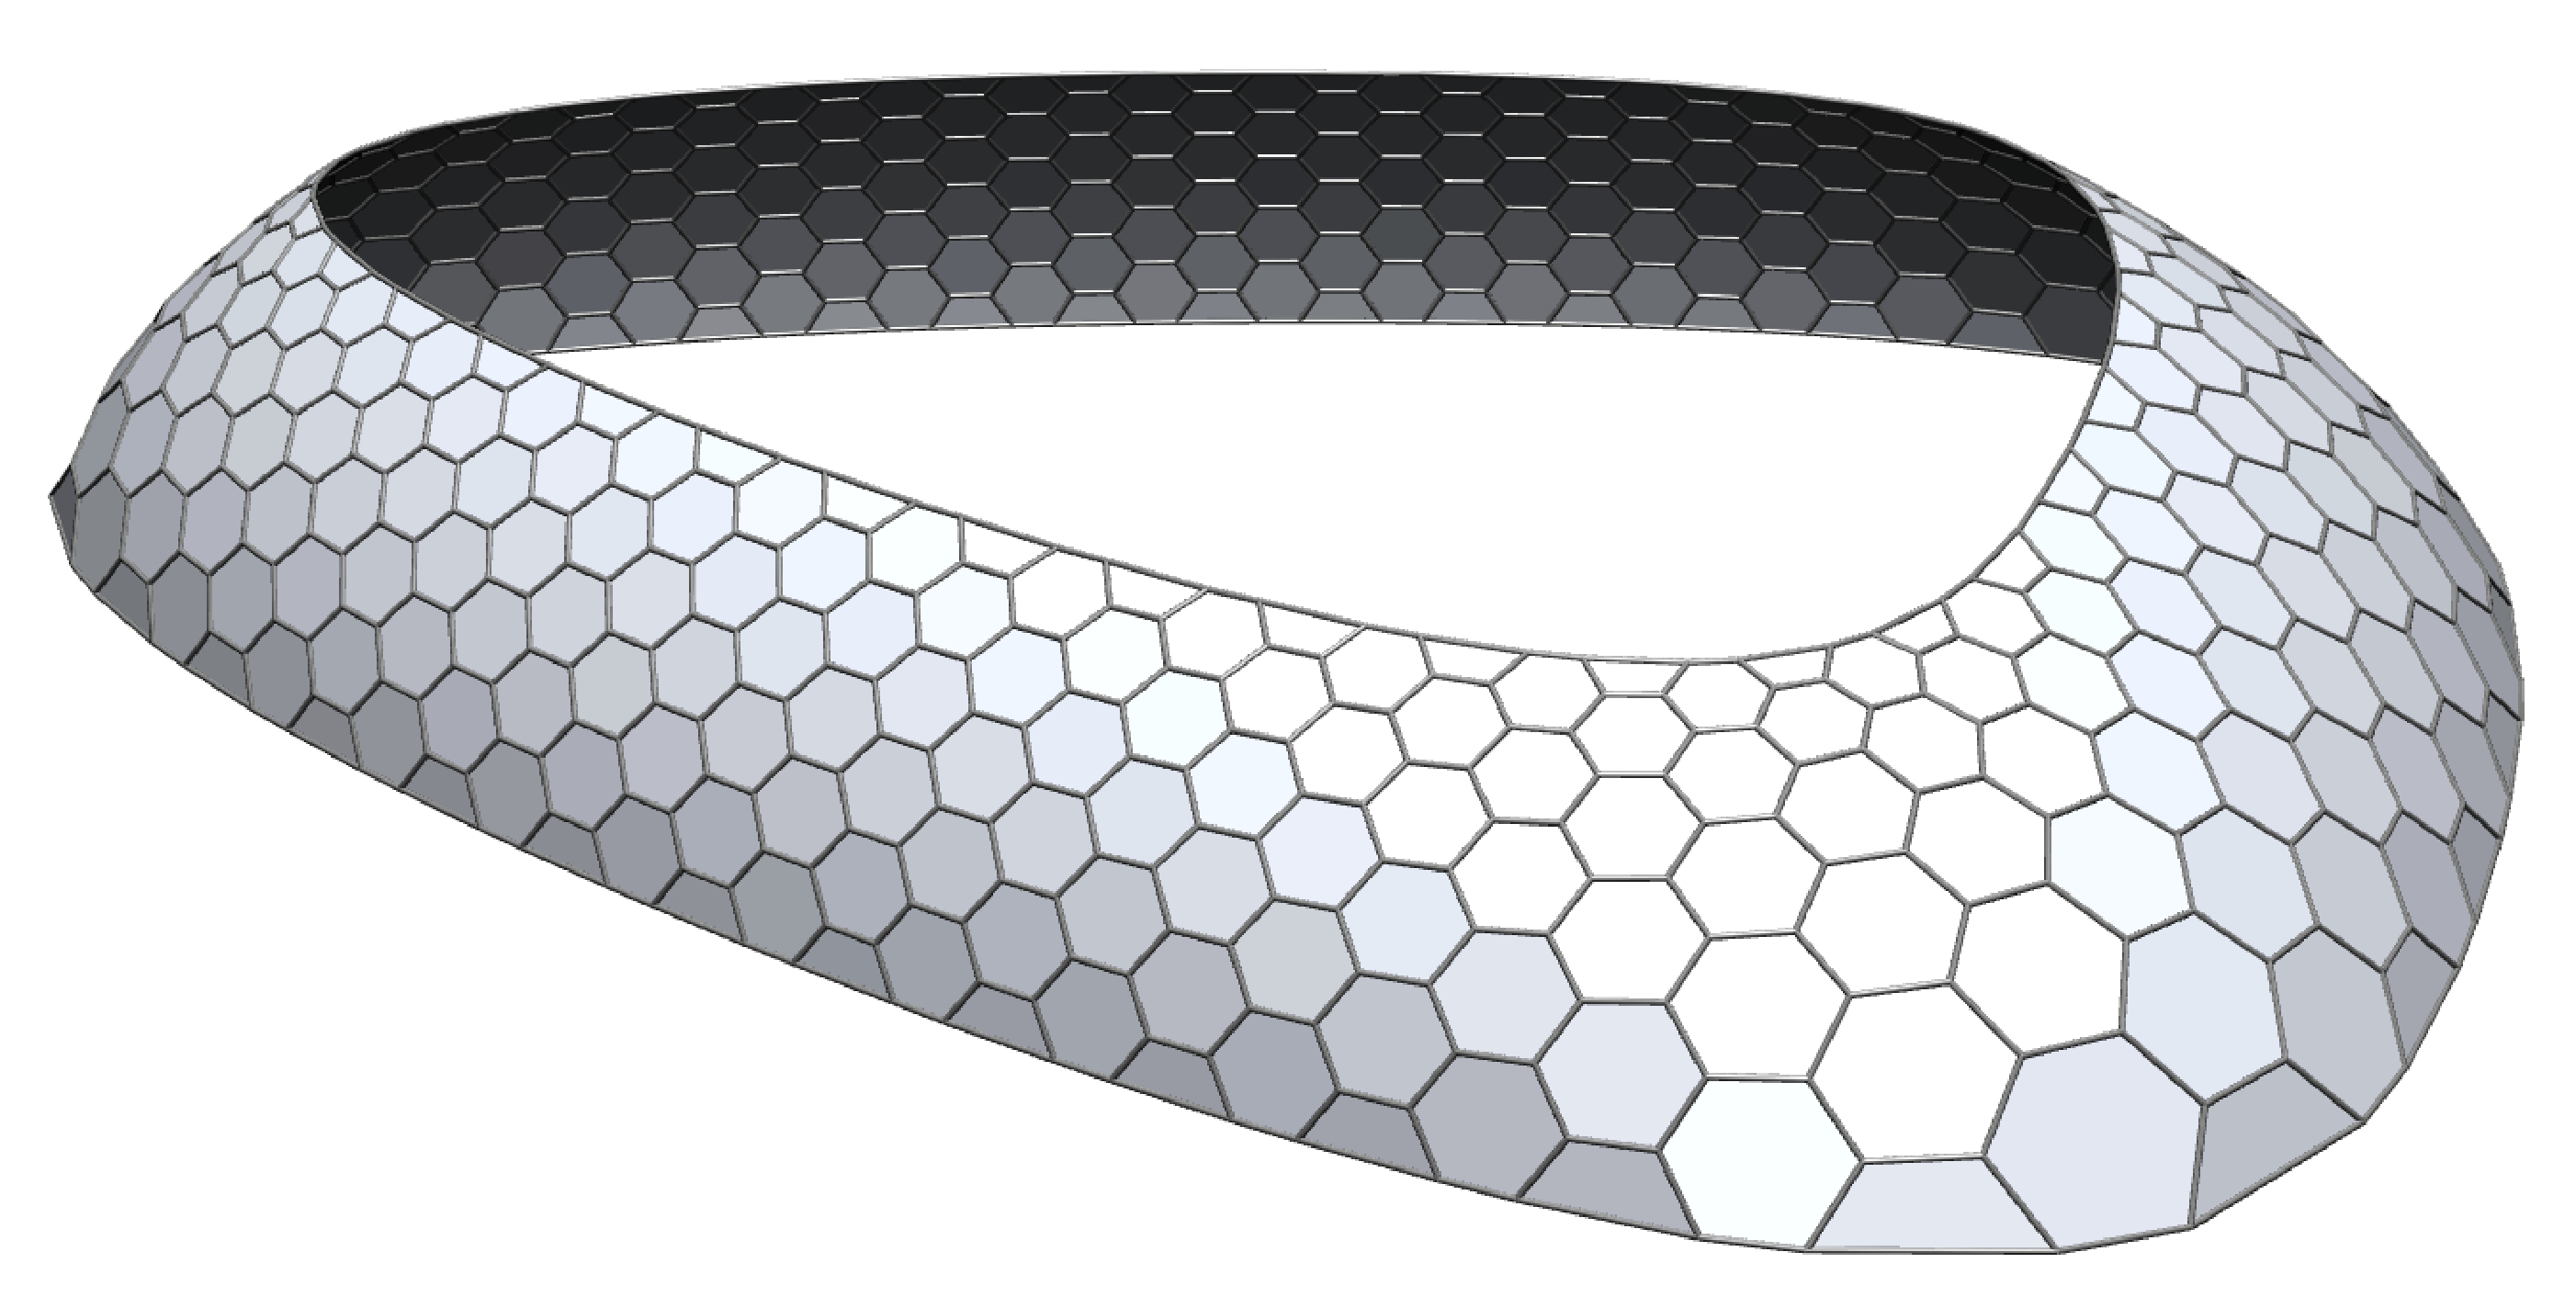
\includegraphics{periodic/step07.pdf}	
            }
            \captionof{figure}{Creating a periodic hexagonal mesh from a triangle mesh.}
\end{minipage}
\end{center}                
\end{compactenum}

\subsection{Panel optimization}

\begin{compactenum}[(1)]
\item[(7)] \emph{Topology$\to$Explode} creates separate faces. We use a \emph{Mean Face Edge Length} histogram to show the density of edge lengths. If we want planar panels we should planarize them now.

\begin{center}
\begin{minipage}{0.9\linewidth}
            \centering
            \resizebox{\linewidth}{!}{
            	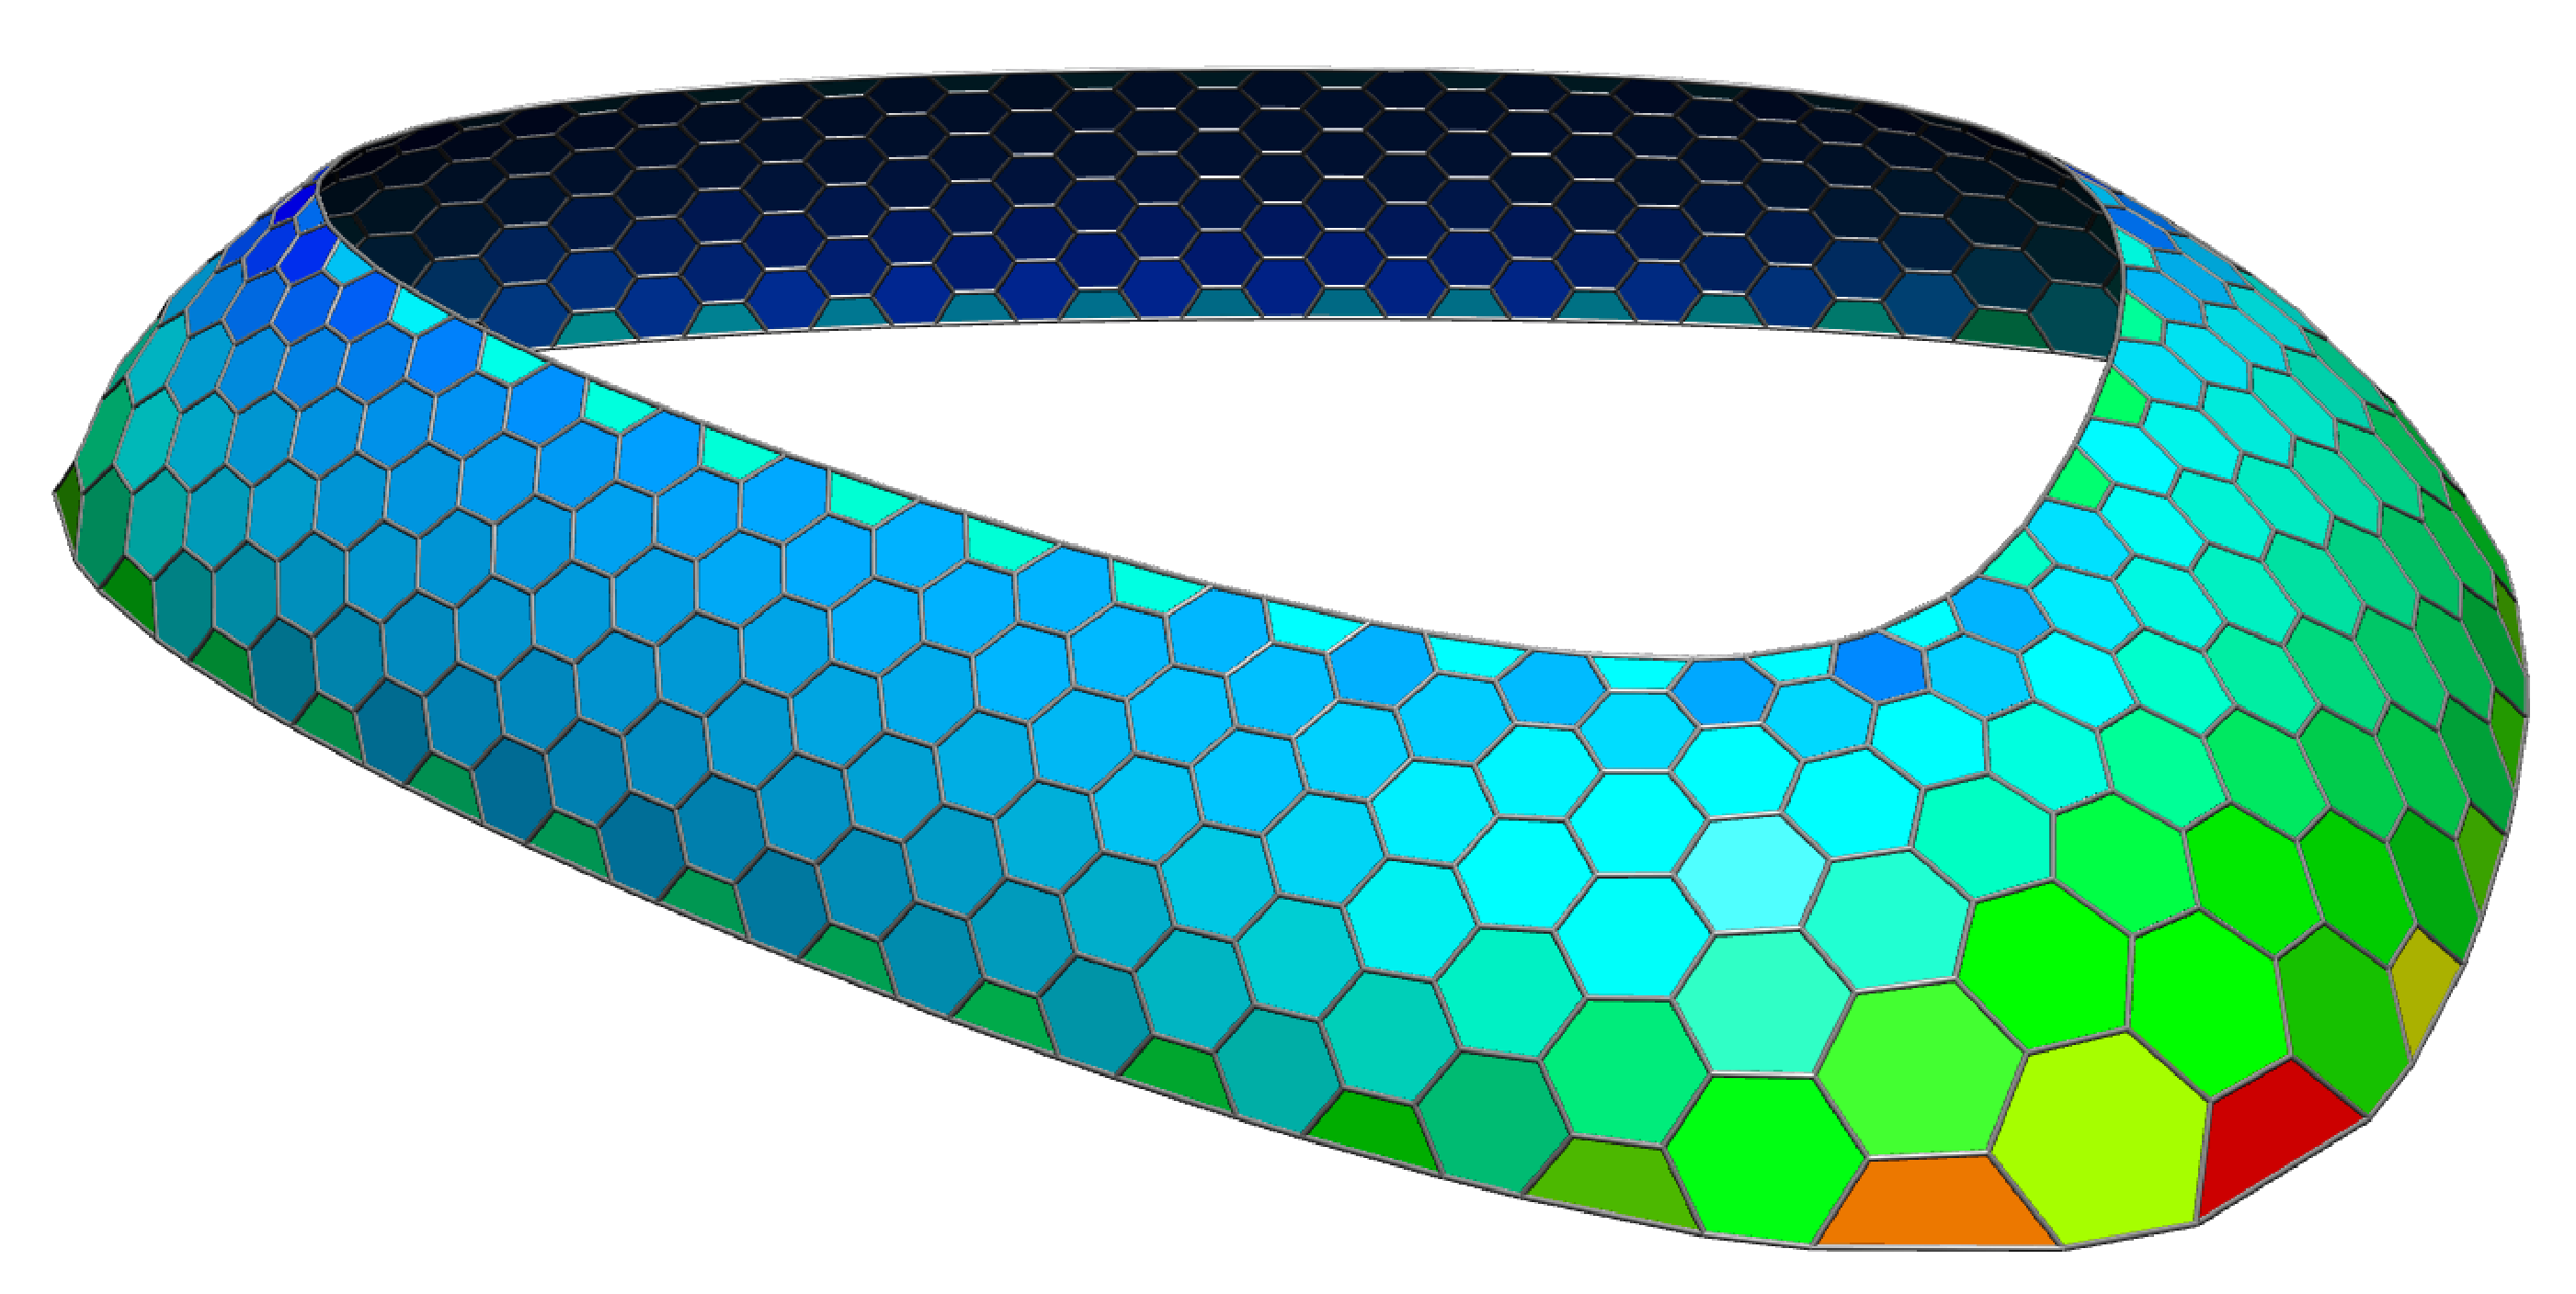
\includegraphics[width=5cm]{periodic/step08_surface.pdf}
            	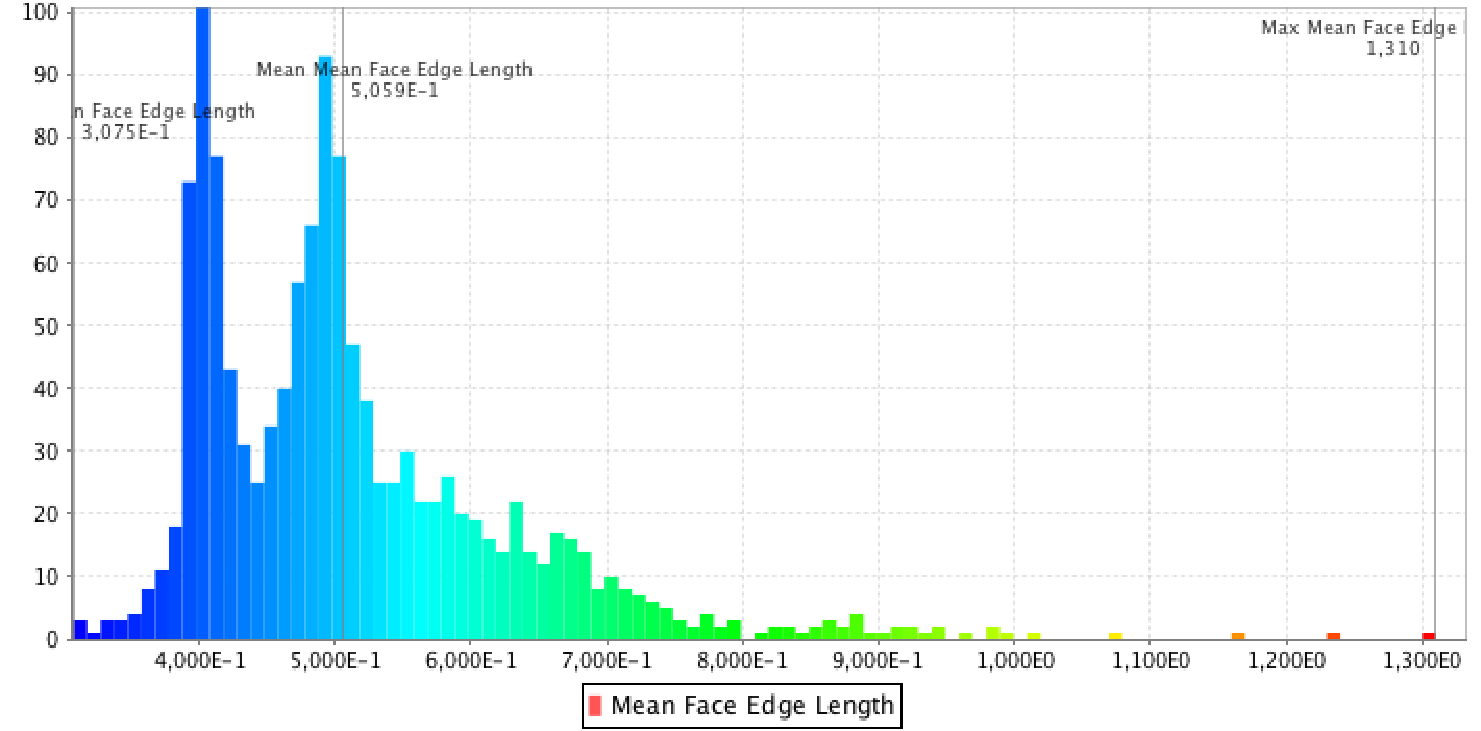
\includegraphics[width=5cm]{periodic/step08_histogram.pdf}		
            }
            \captionof{figure}{Measuring panel sizes and density with the \emph{Halfedge Data Visualization} facility.}
\end{minipage}
\end{center}

\item[(8)] We equalize the edge lengths per face using the \emph{Springs} Energy and \emph{F-const} option. Use the \emph{Floor} rounding method. Press \emph{Update} to set target lengths per face.

\begin{center}
\begin{minipage}{0.9\linewidth}
            \centering
            \resizebox{\linewidth}{!}{
            	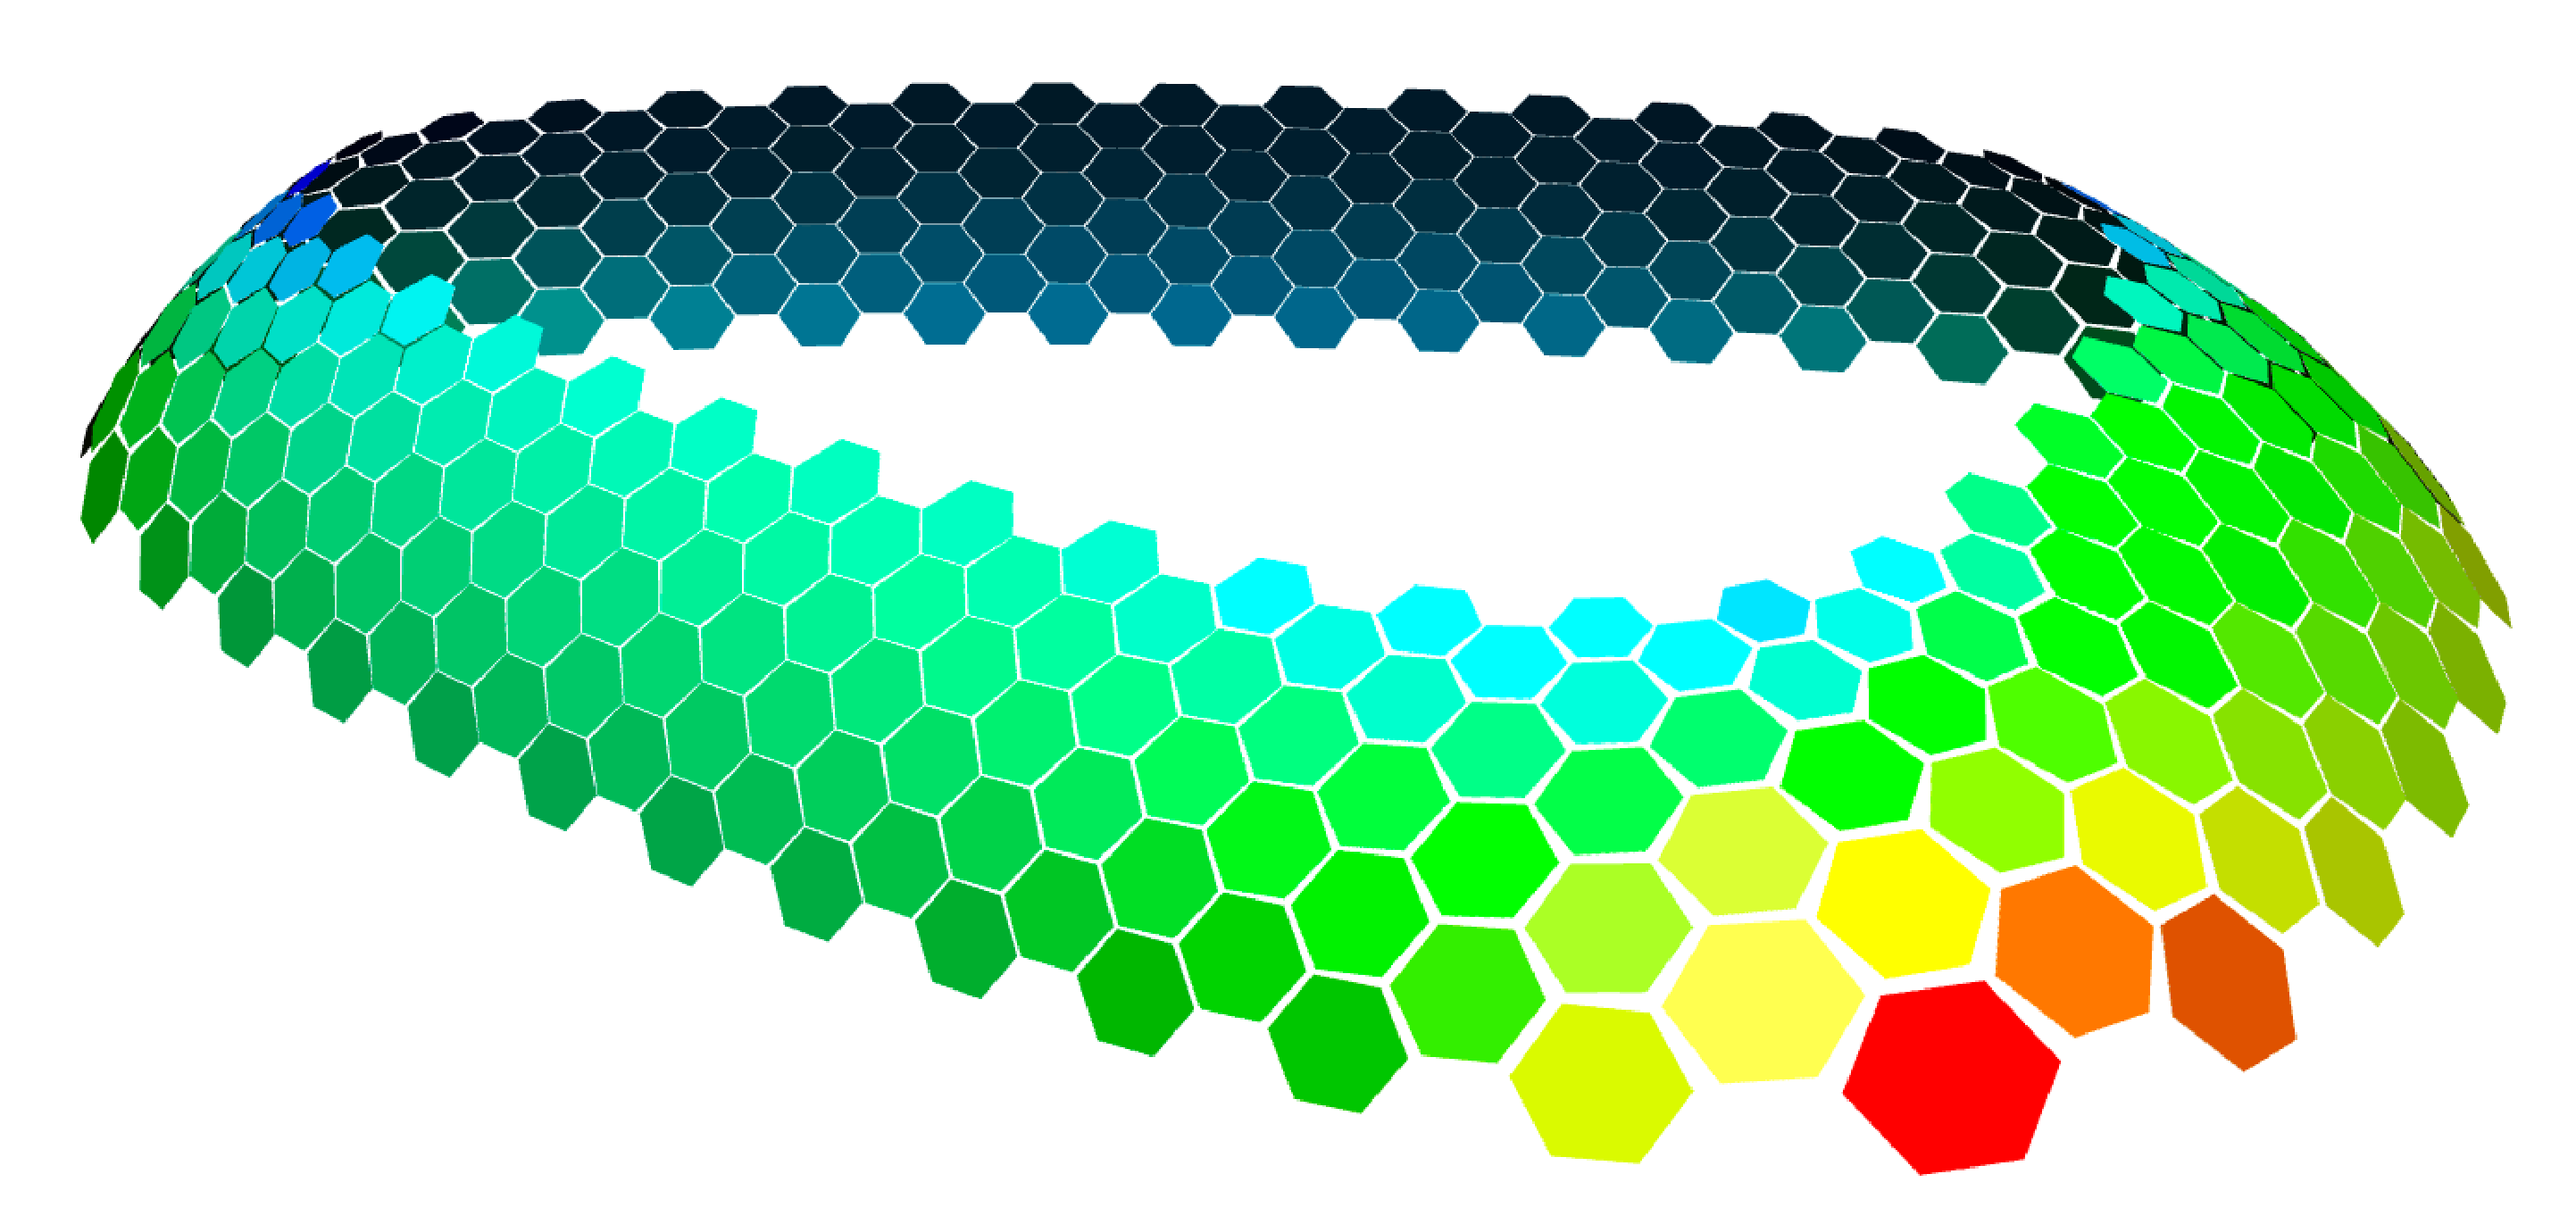
\includegraphics[width=13cm]{periodic/step09_surface.pdf}
            	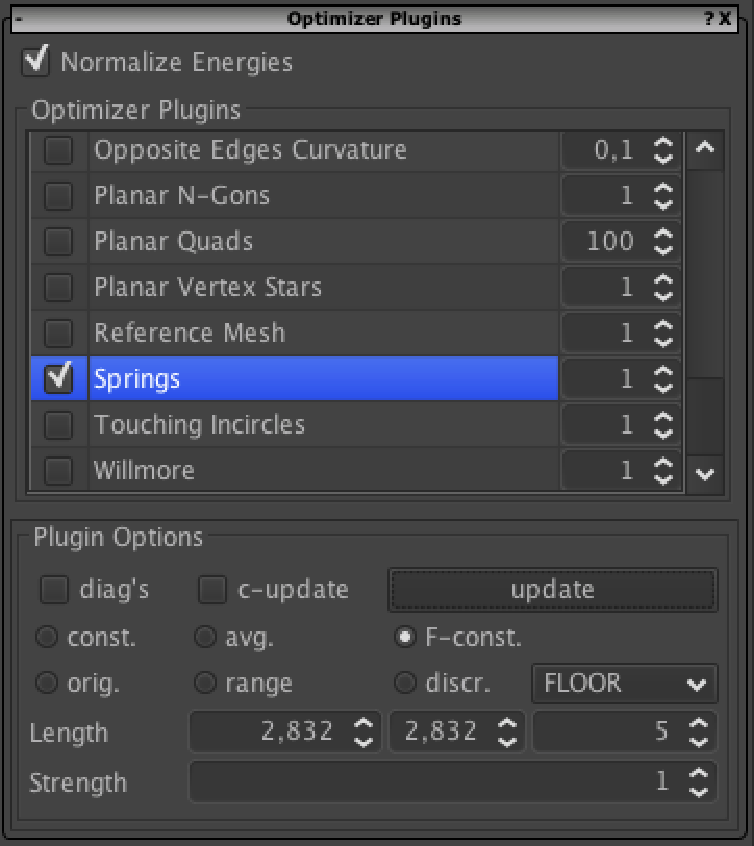
\includegraphics[width=5cm]{periodic/step09_fconst.pdf}
            }
            \captionof{figure}{Creating regular elements with the \emph{Spring} energy.}
\end{minipage}
\end{center}
\item[(9)] From the histogram, read off the smallest and largest edge lengths and transfer those into the \emph{Springs} energy UI. We select the \emph{discr.} option and the number of discrete steps. Optimize the surface to consist of a limited number of panel sizes.

\begin{center}
\begin{minipage}{0.9\linewidth}
            \centering
            \resizebox{\linewidth}{!}{
            	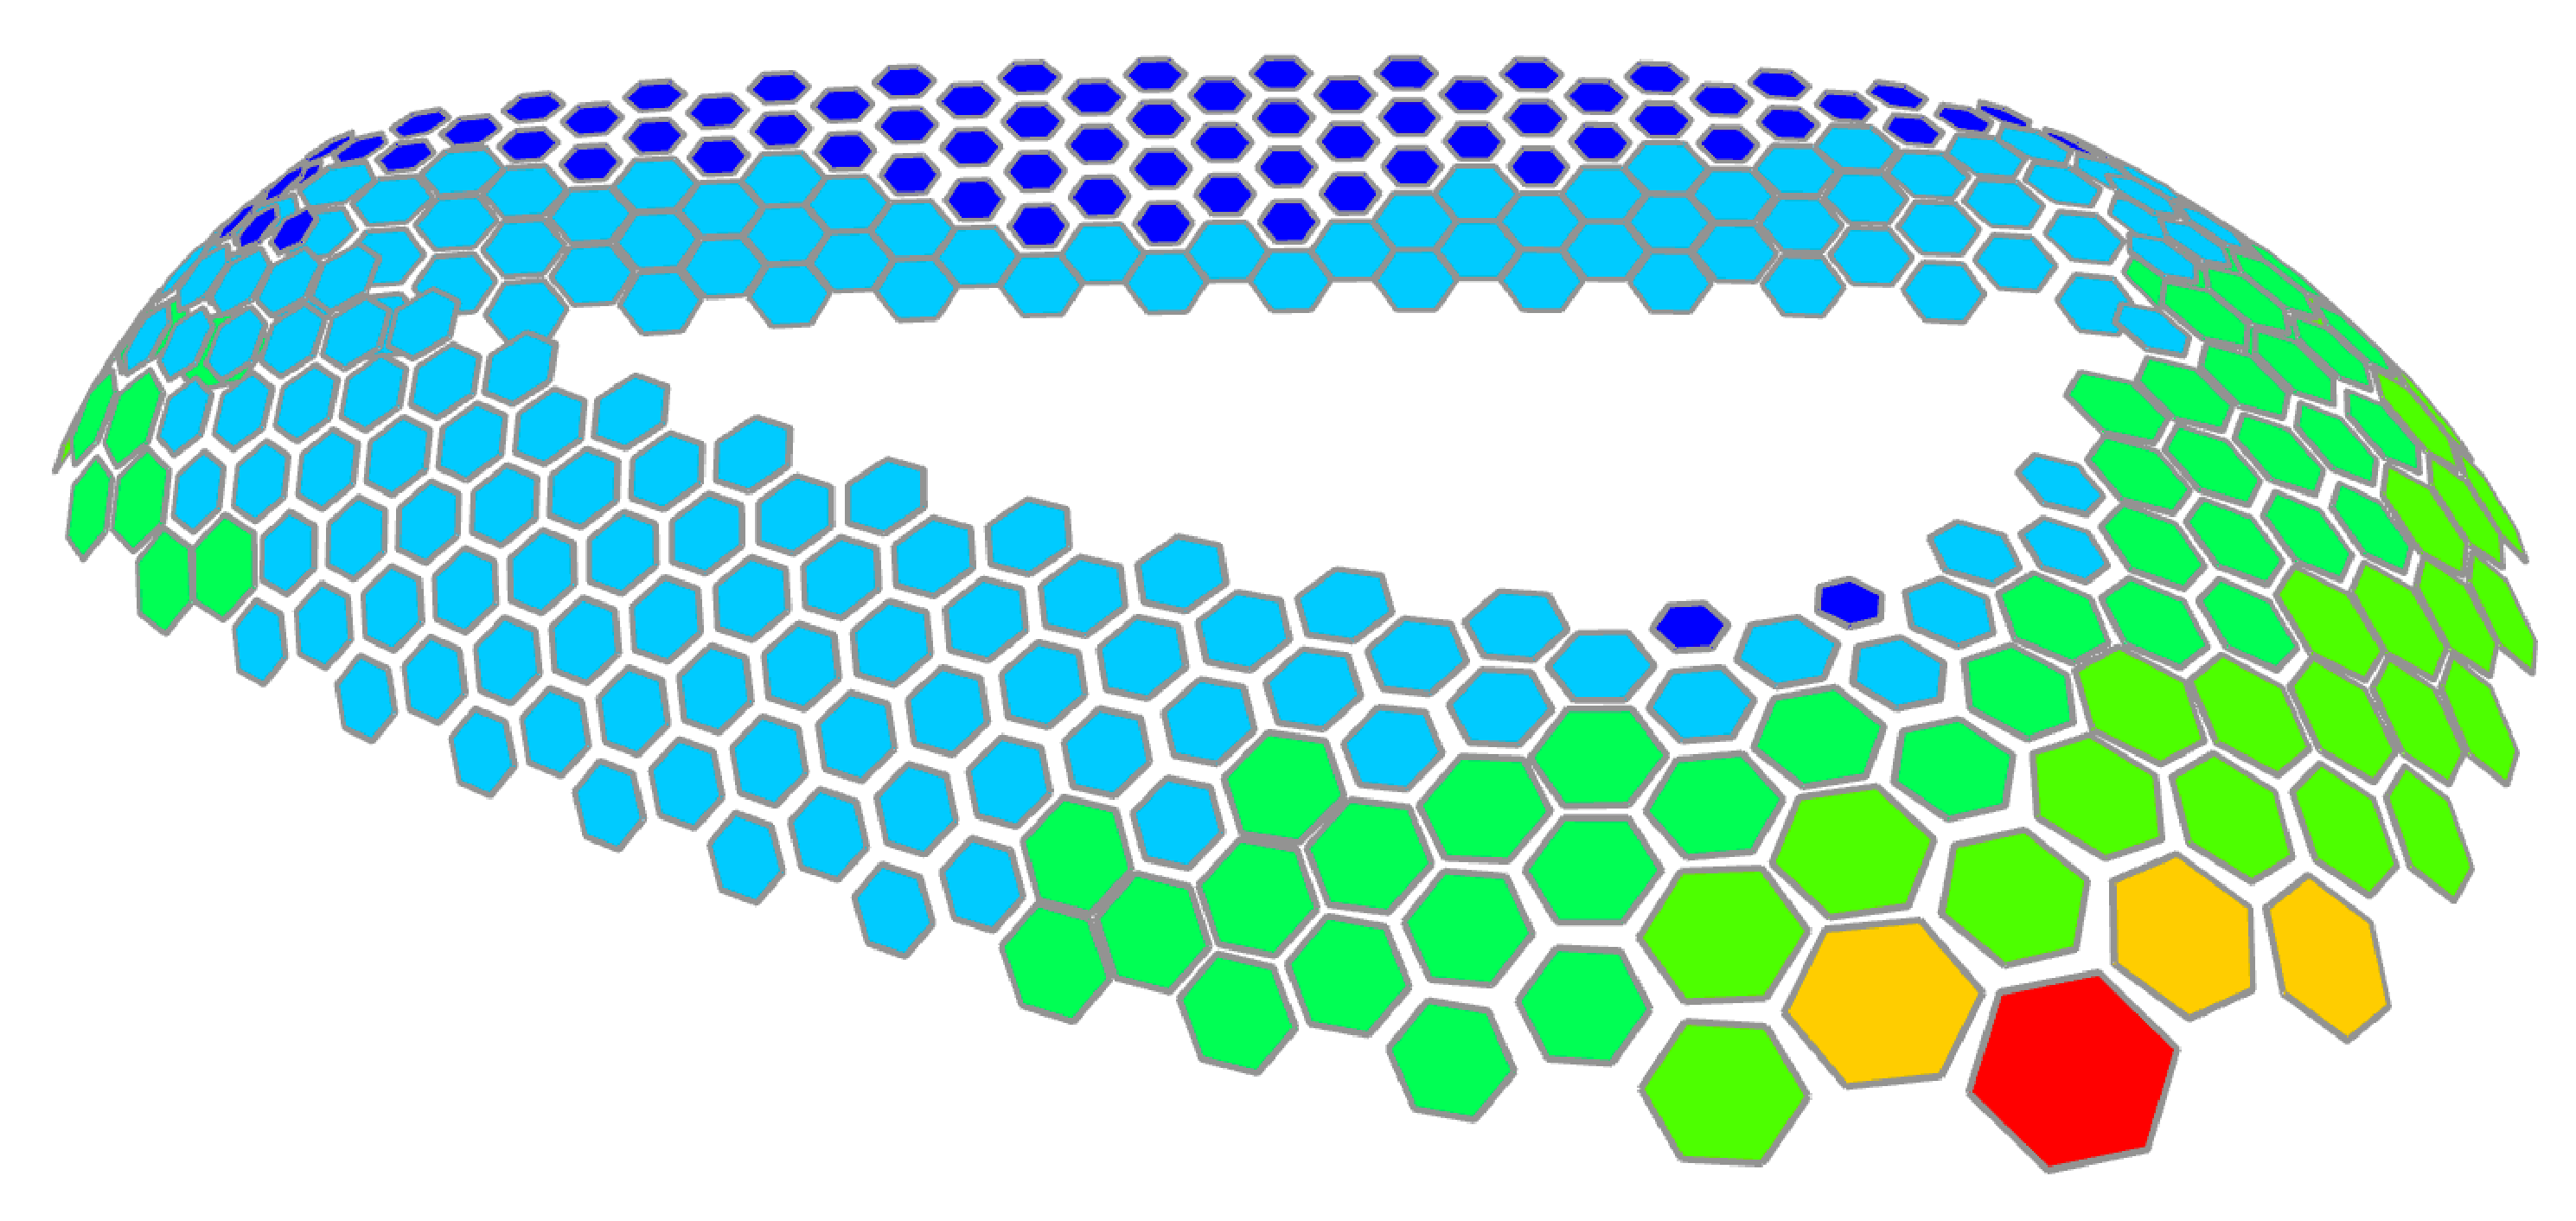
\includegraphics[width=13cm]{periodic/step11_surface1.pdf}
            	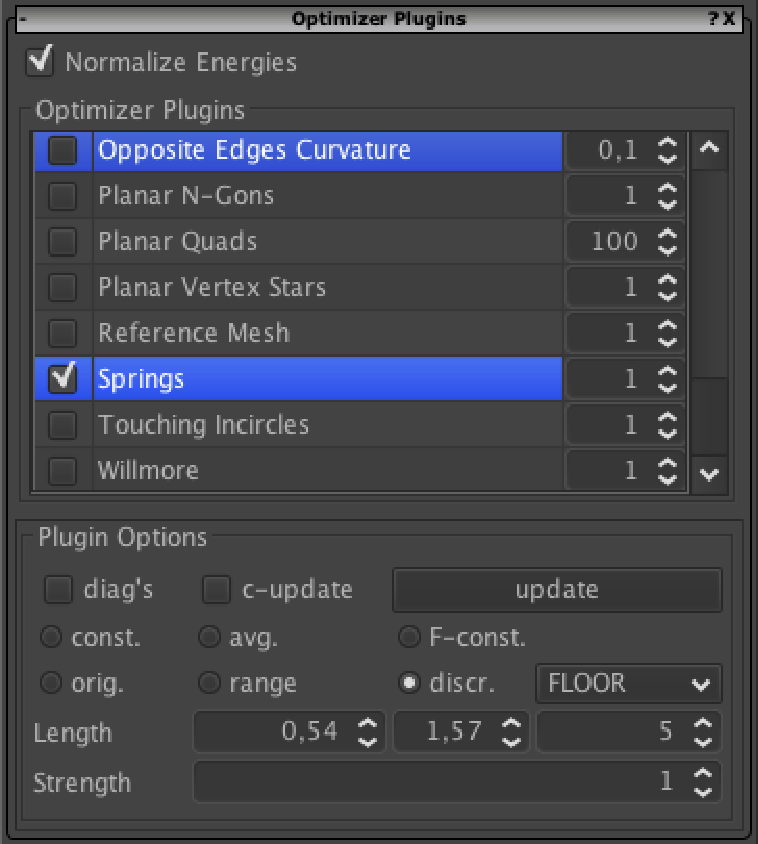
\includegraphics[width=5cm]{periodic/step10_springs.pdf}
            }
            \captionof{figure}{Optimization towards a discrete set of panel sizes.}
\end{minipage}
\end{center}            
\end{compactenum}



\section{Quasiisothermic meshes with {\sc VaryLab}}
\label{sec:quasiisothermic_varylab}

The methods of Chapter~\ref{chp:quasiisothermic} can be divided into two parts. The Parameterization part where we create the coordinates of the triangle mesh based on curvature direction data on the boundary of the mesh. And the optimization part where a quadrilateral mesh from part 1 is optimized towards touching incircles, the defining property of discrete s-isothermic meshes.

\subsection{Quasiisothermic paramerization}

\begin{compactenum}[(1)]
\item[(0)] We load a genus-$0$ surface with one boundary component.
\item[(1)] Calculate curvature direction estimates on interior vertices to find singularity locations and indices with the \emph{Vector Field$\to$Curvature Vector Fields} command. We visualize directions using the \emph{Halfedge Data Visualization} interface. The data is called, e.g., \emph{Kmax Vec V} for maximum curvature direction with respect to the surface normal.
\item[(2)] We select singularity vertices and assign corresponding cone angles in the \emph{Selected Nodes} panel of the \emph{Discrete Conformal Parameterization} panel.
\item[(3)] Calculate curvature direction estimates on boundary edges of the surface, again using the \emph{Vector Field$\to$Curvature Vector Fields} command. We check singularity indices with the \emph{Check Gau{\ss}-Bonnet} button in the \emph{Discrete Conformal Parameterization} panel. It prints the left side of the Gau{\ss}-Bonnet equation to the console. It should give $2\pi$ for a genus $0$ surface in this case.

\begin{center}
\begin{minipage}{0.9\linewidth}
            \centering
            \resizebox{\linewidth}{!}{
%                \includegraphics[width=5cm]{quasiisothermic/step00.pdf}
                \includegraphics[height=5cm]{quasiisothermic/step02_surface.pdf}
                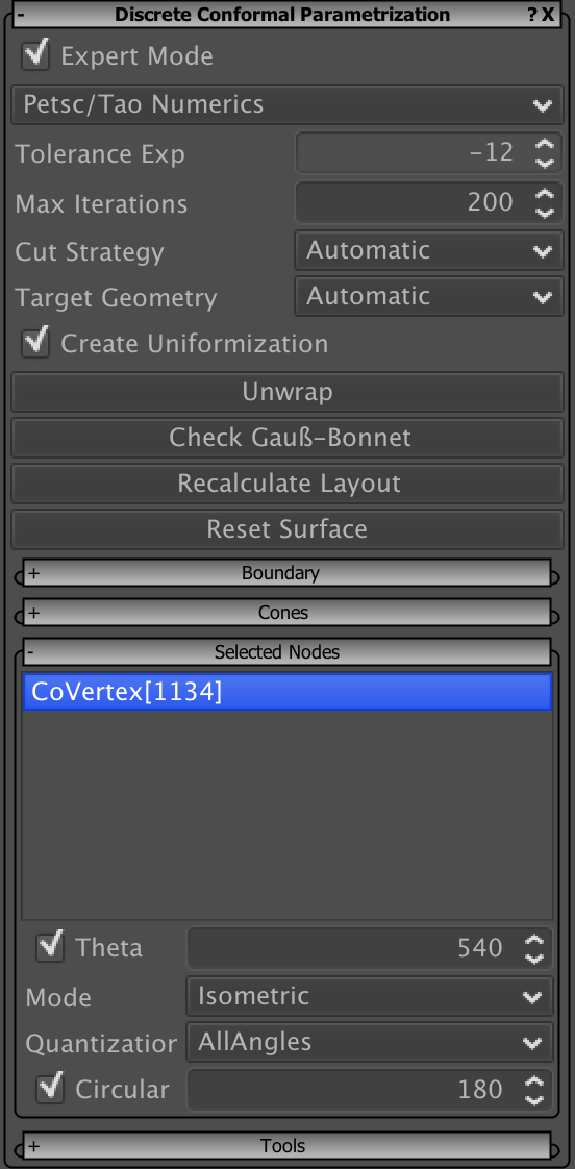
\includegraphics[height=5cm]{quasiisothermic/step02_ui.pdf}
                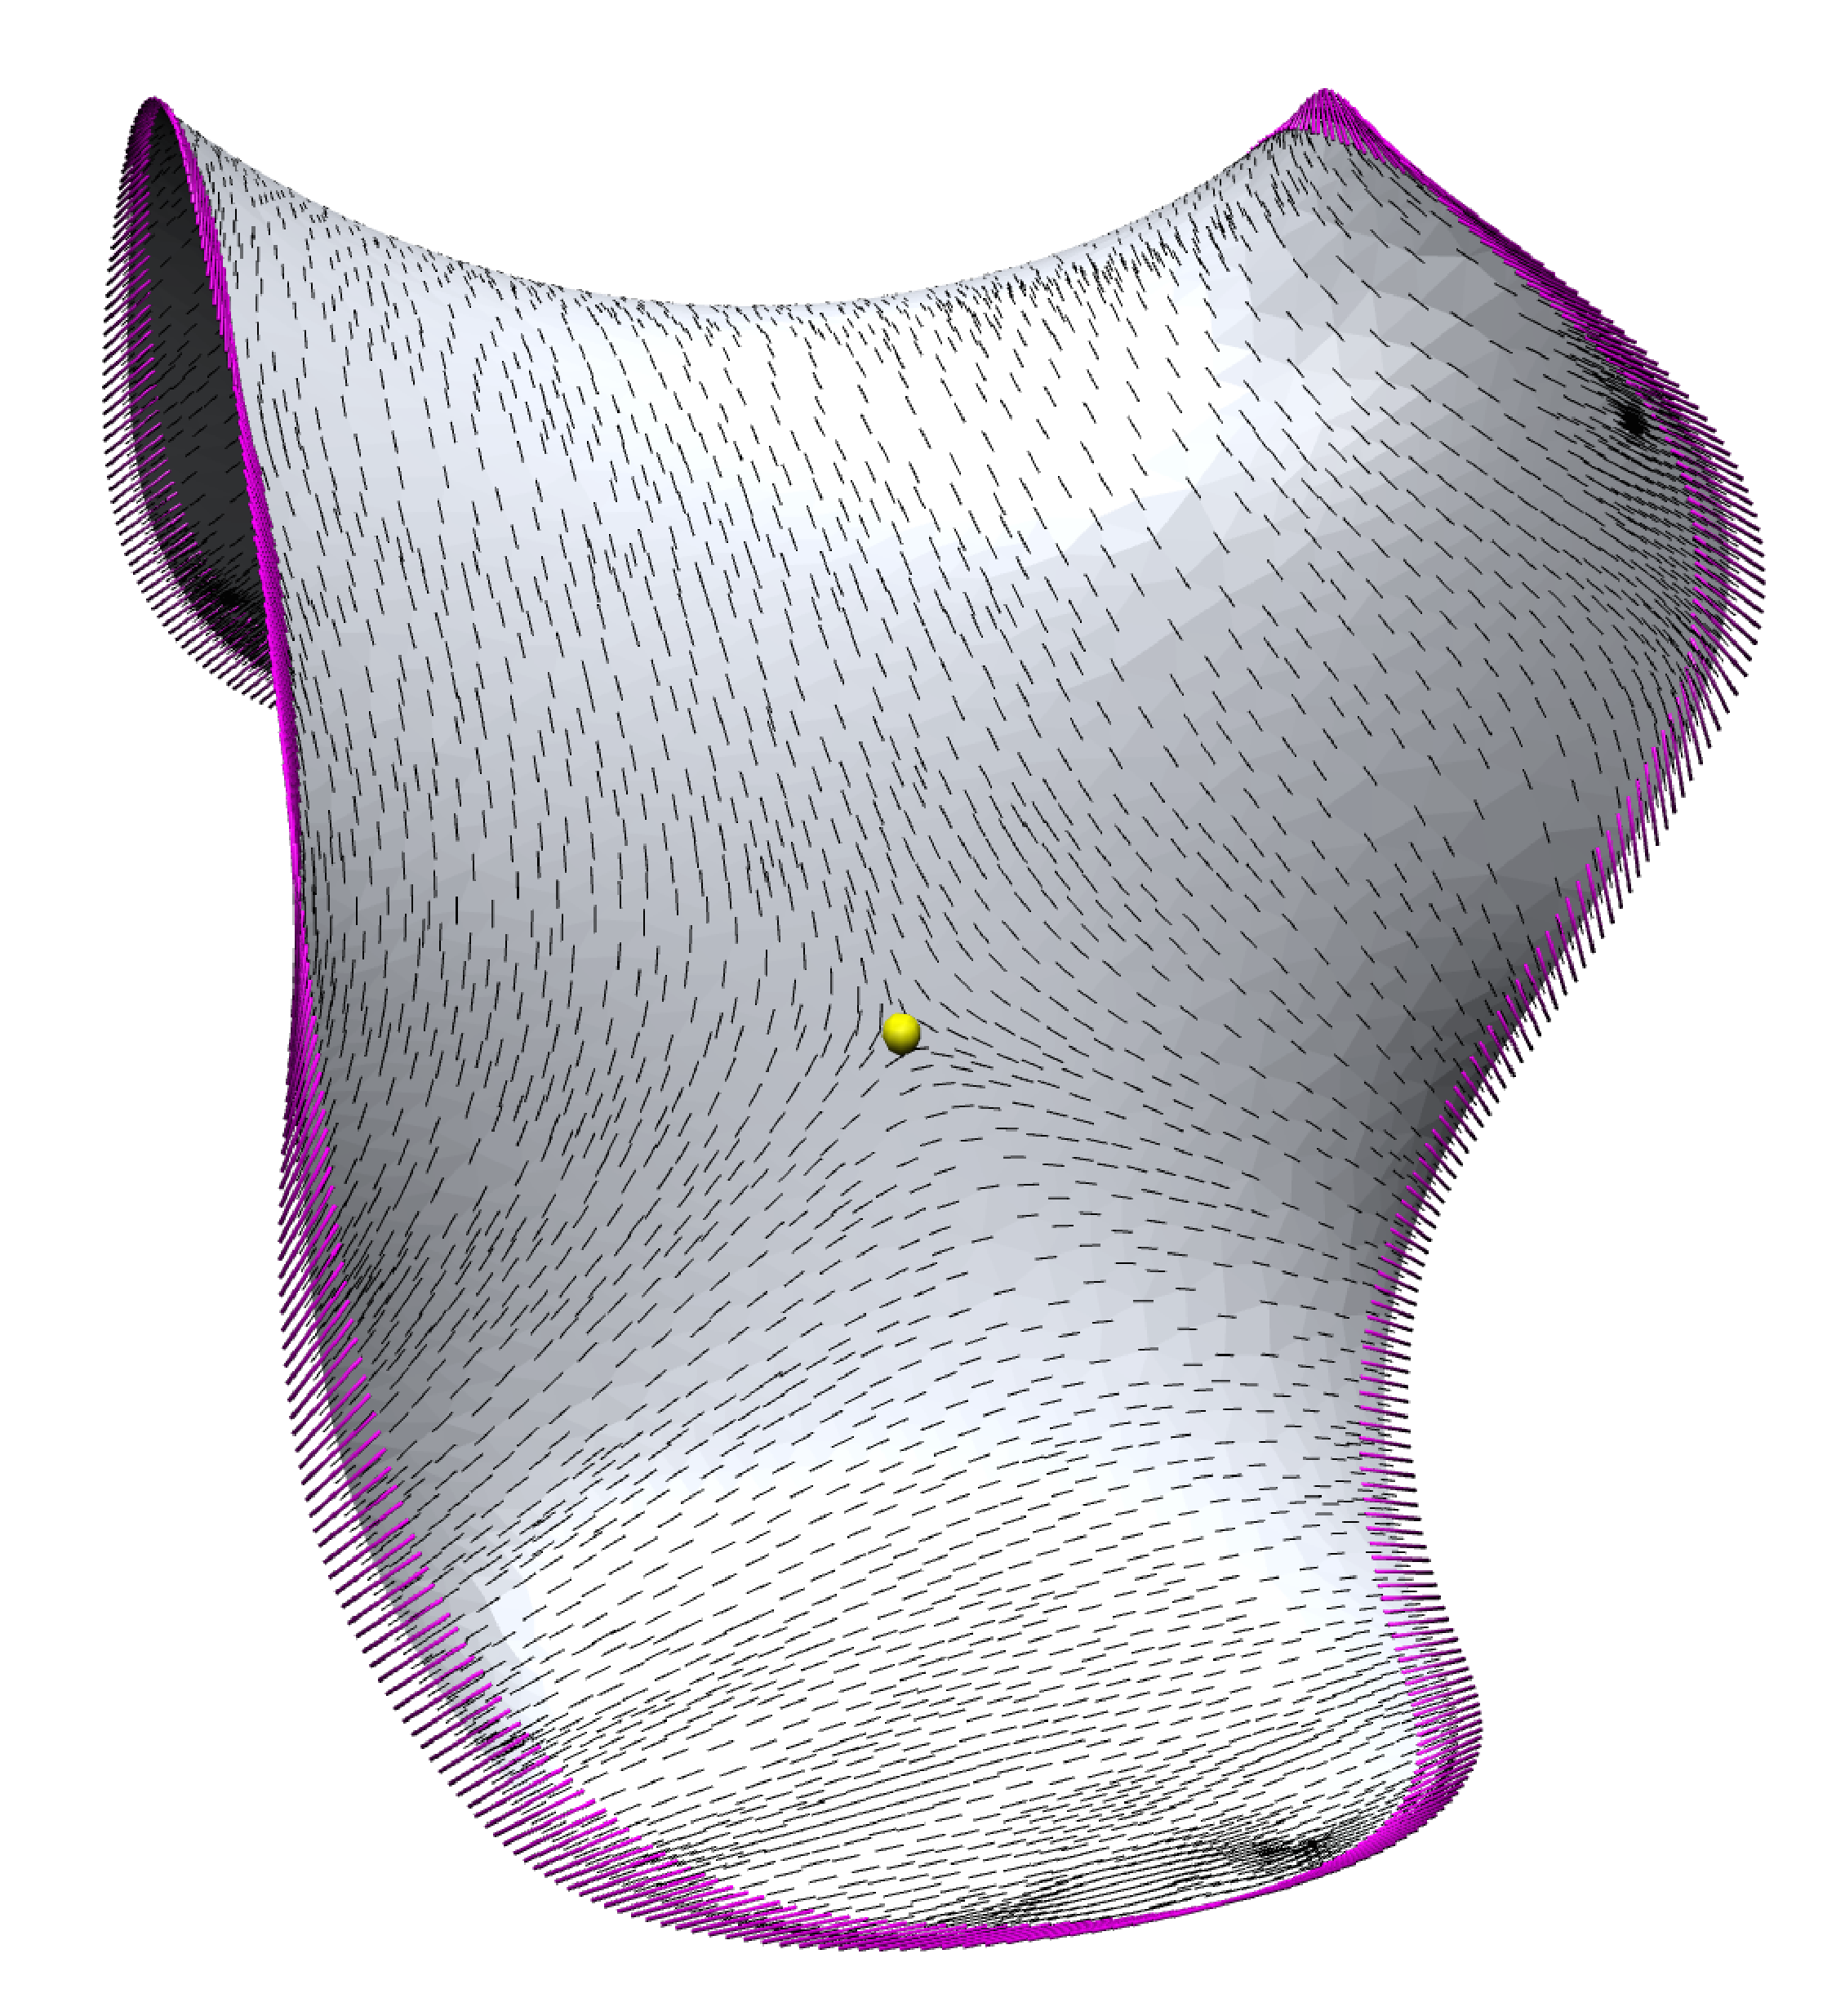
\includegraphics[height=5cm]{quasiisothermic/step03_surface.pdf}
            }
            \captionof{figure}{Inspect the curvature direction field on the surface (left) and specify boundary conditions (right, magenta) and singularities (right, yellow).}
\end{minipage}
\end{center}     
            
\item[(4)] Create a discrete conformal parameterization. We use \emph{Conformal Curvature} as boundary mode. Select a quad texture to visualize the parameterization on the surface. Rotate the texture to match the prescribed boundary directions.
\item[(5)] Move the texture such that singularities lie either in the middle or at a corner of a quad of the texture. Use the \emph{Texture Remeshing$\to$Transform Texture} command to transform the texture such that two selected vertices lie on $(0,0)$ and $(1,0)$ respectively. This method works for one or two singularities. We do not implement methods to distort the mapping to match more that two singularities.

\begin{center}
\begin{minipage}{0.9\linewidth}
            \centering
            \resizebox{\linewidth}{!}{
                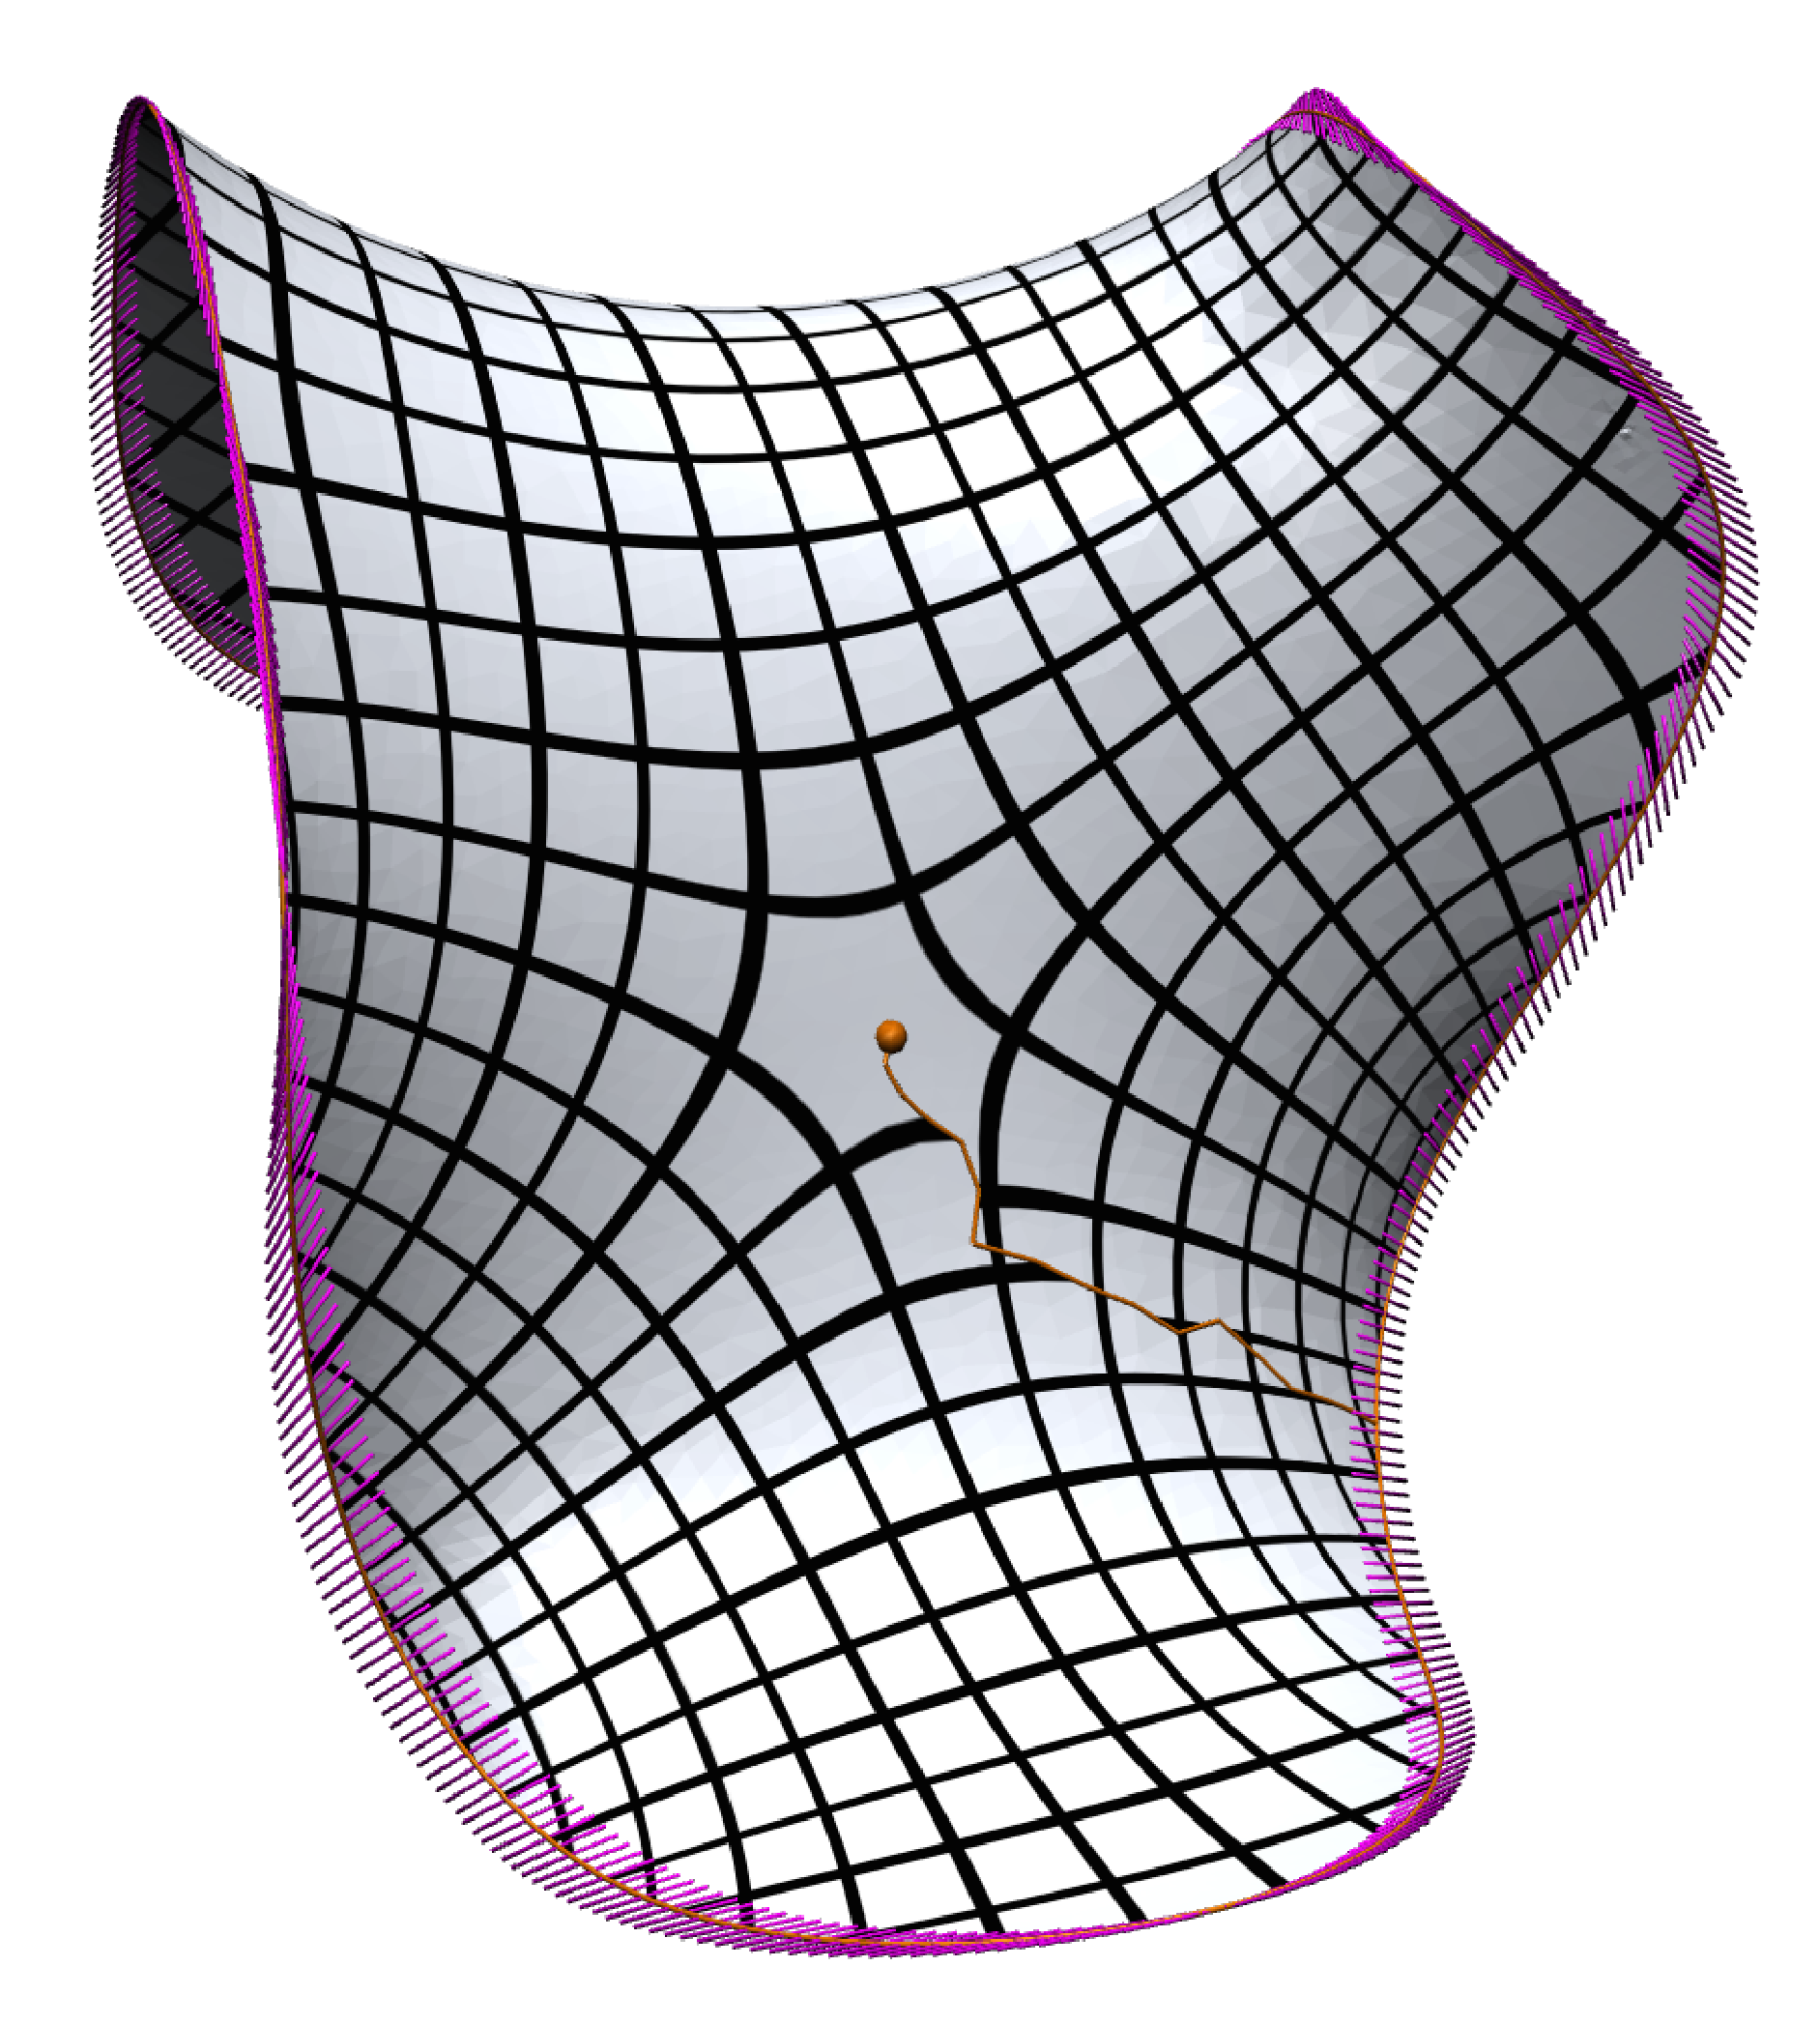
\includegraphics[width=5cm]{quasiisothermic/step04_surface.pdf}
                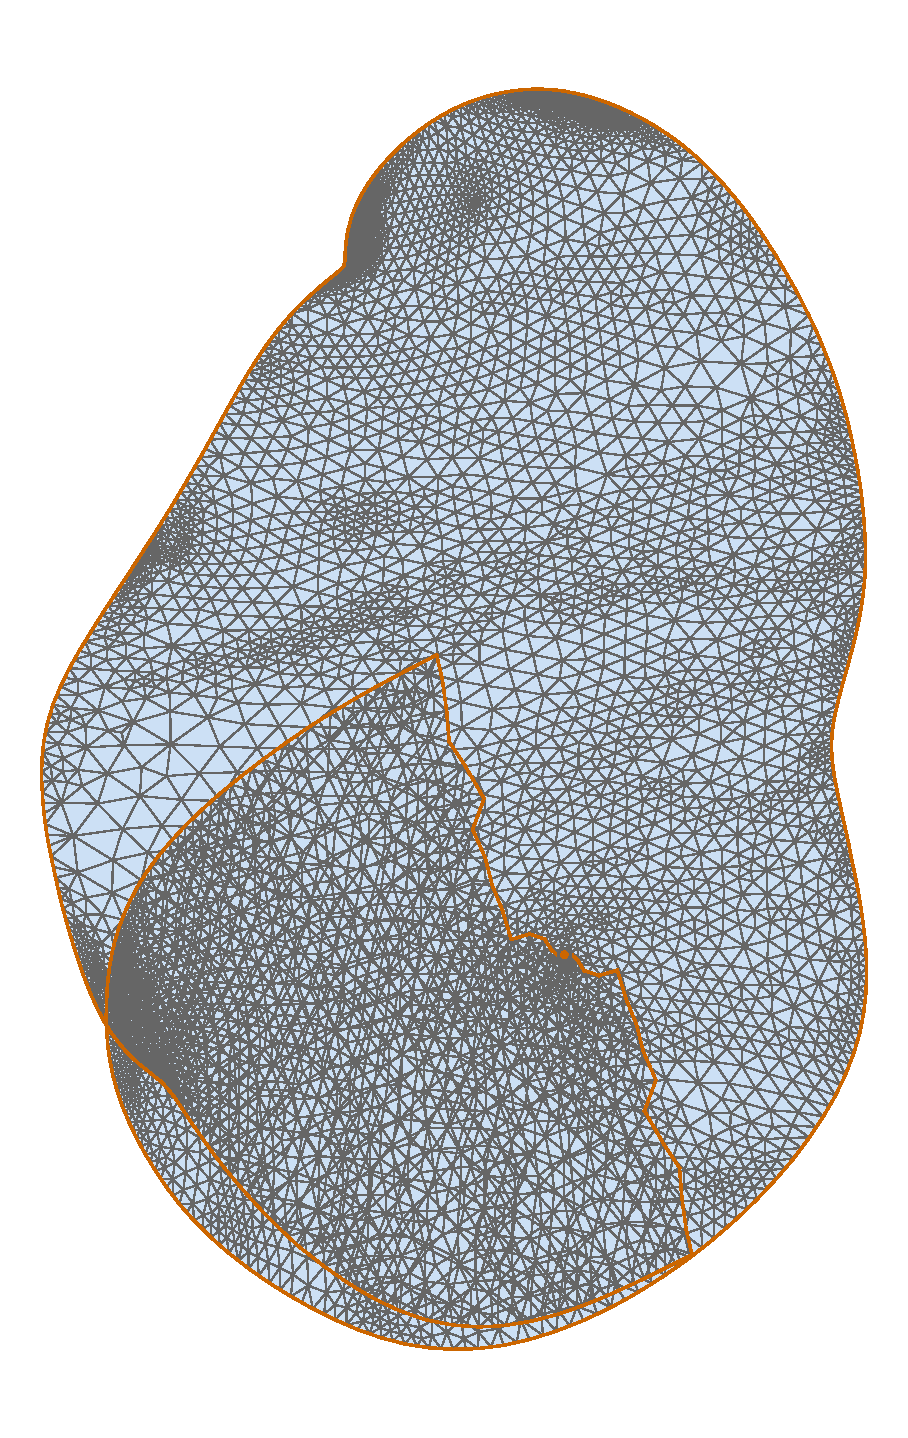
\includegraphics[width=4cm]{quasiisothermic/step04_map.pdf}
                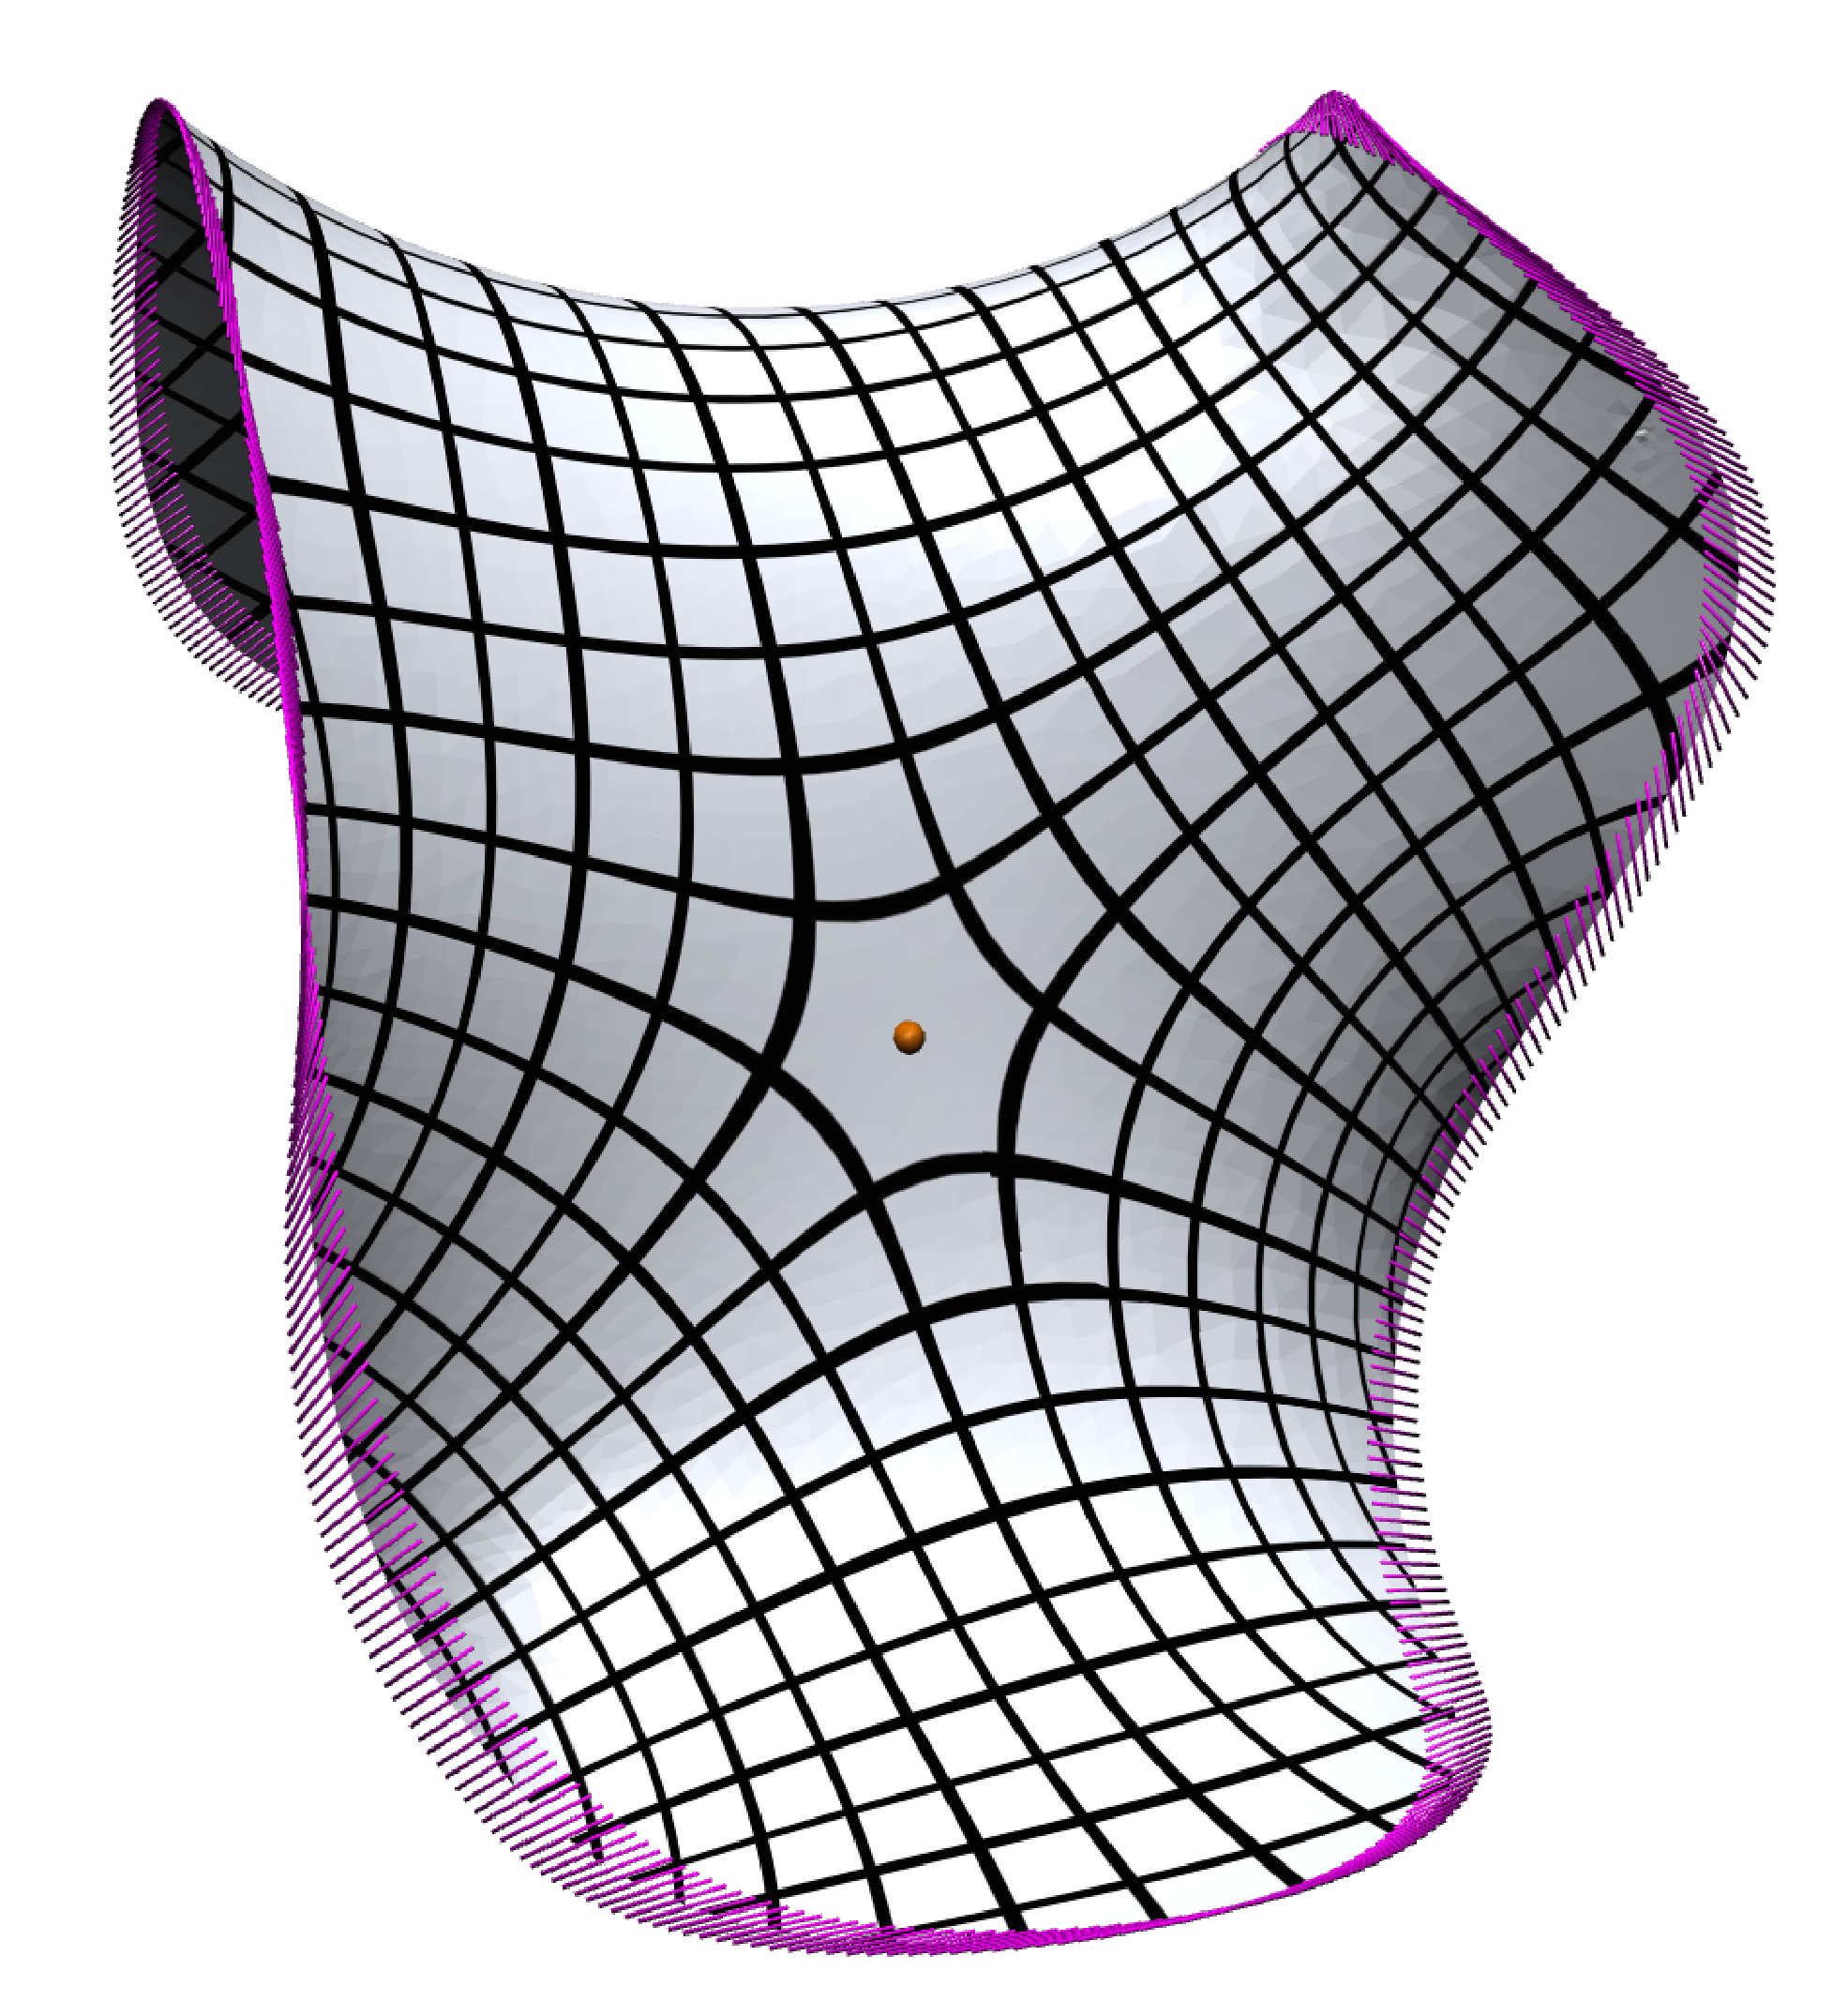
\includegraphics[width=5cm]{quasiisothermic/step05_surface.pdf}
            }
            \captionof{figure}{A quasiisothermic parameterization and its domain (left and middle). Move the singularity to a symmetry point of the pattern to close the parameter lines on the surface.}
\end{minipage}
\end{center}     
            
\item[(6)] Create a subdivision quad-mesh using the \emph{Surface Remeshing} panel and the \emph{Quads With Singularities} mode. This mode is available in the \emph{Expert} mode of the panel. Press the \emph{Lift/Flat} button to lift the subdivision to the surface.
\item[(7)] Use the \emph{Texture Remeshing$\to$TextureGeometry} command to extract a quad mesh from the subdivision mesh. Disable the layer of the original mesh as we will continue to work with the quad-mesh.

\begin{center}
\begin{minipage}{0.9\linewidth}
            \centering
            \resizebox{\linewidth}{!}{
                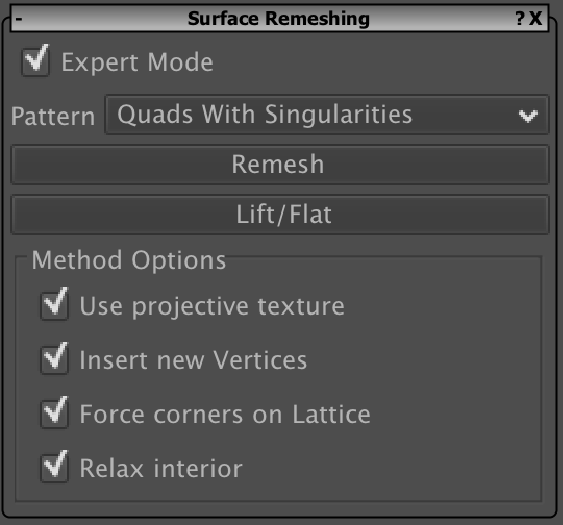
\includegraphics[width=4cm]{quasiisothermic/step06_ui.pdf}
                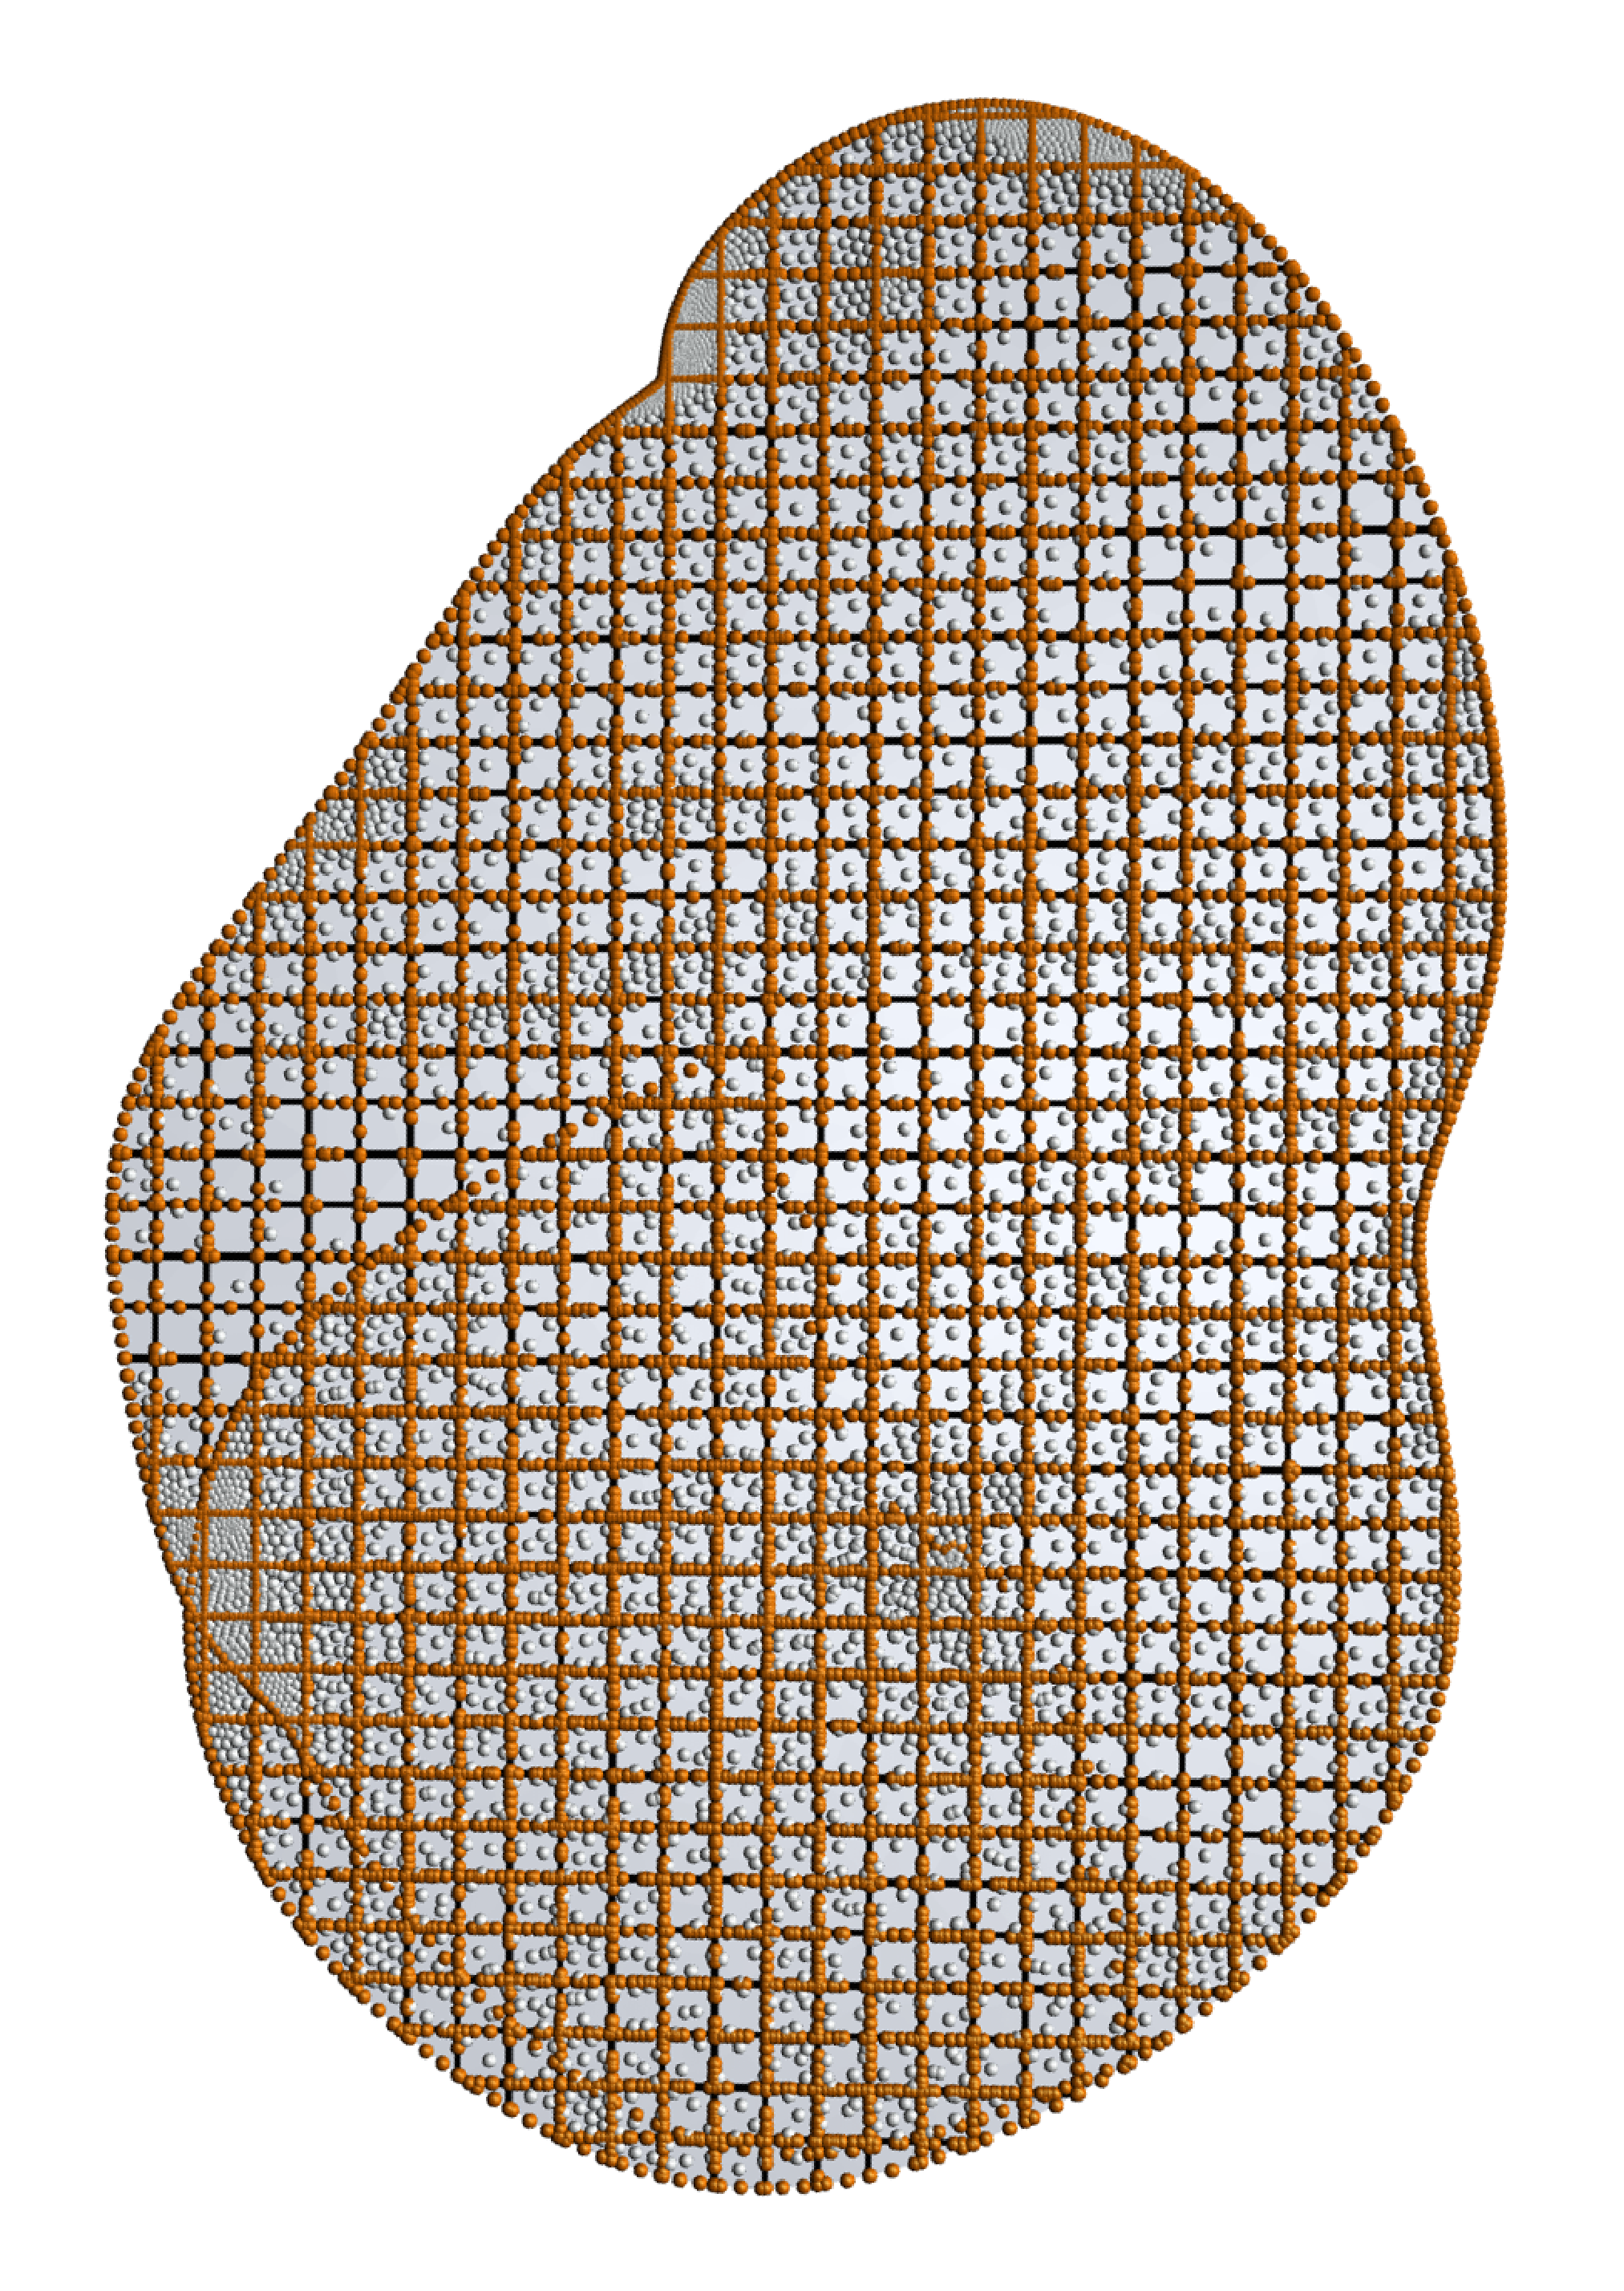
\includegraphics[width=4cm]{quasiisothermic/step06_flat_rotate.pdf}
                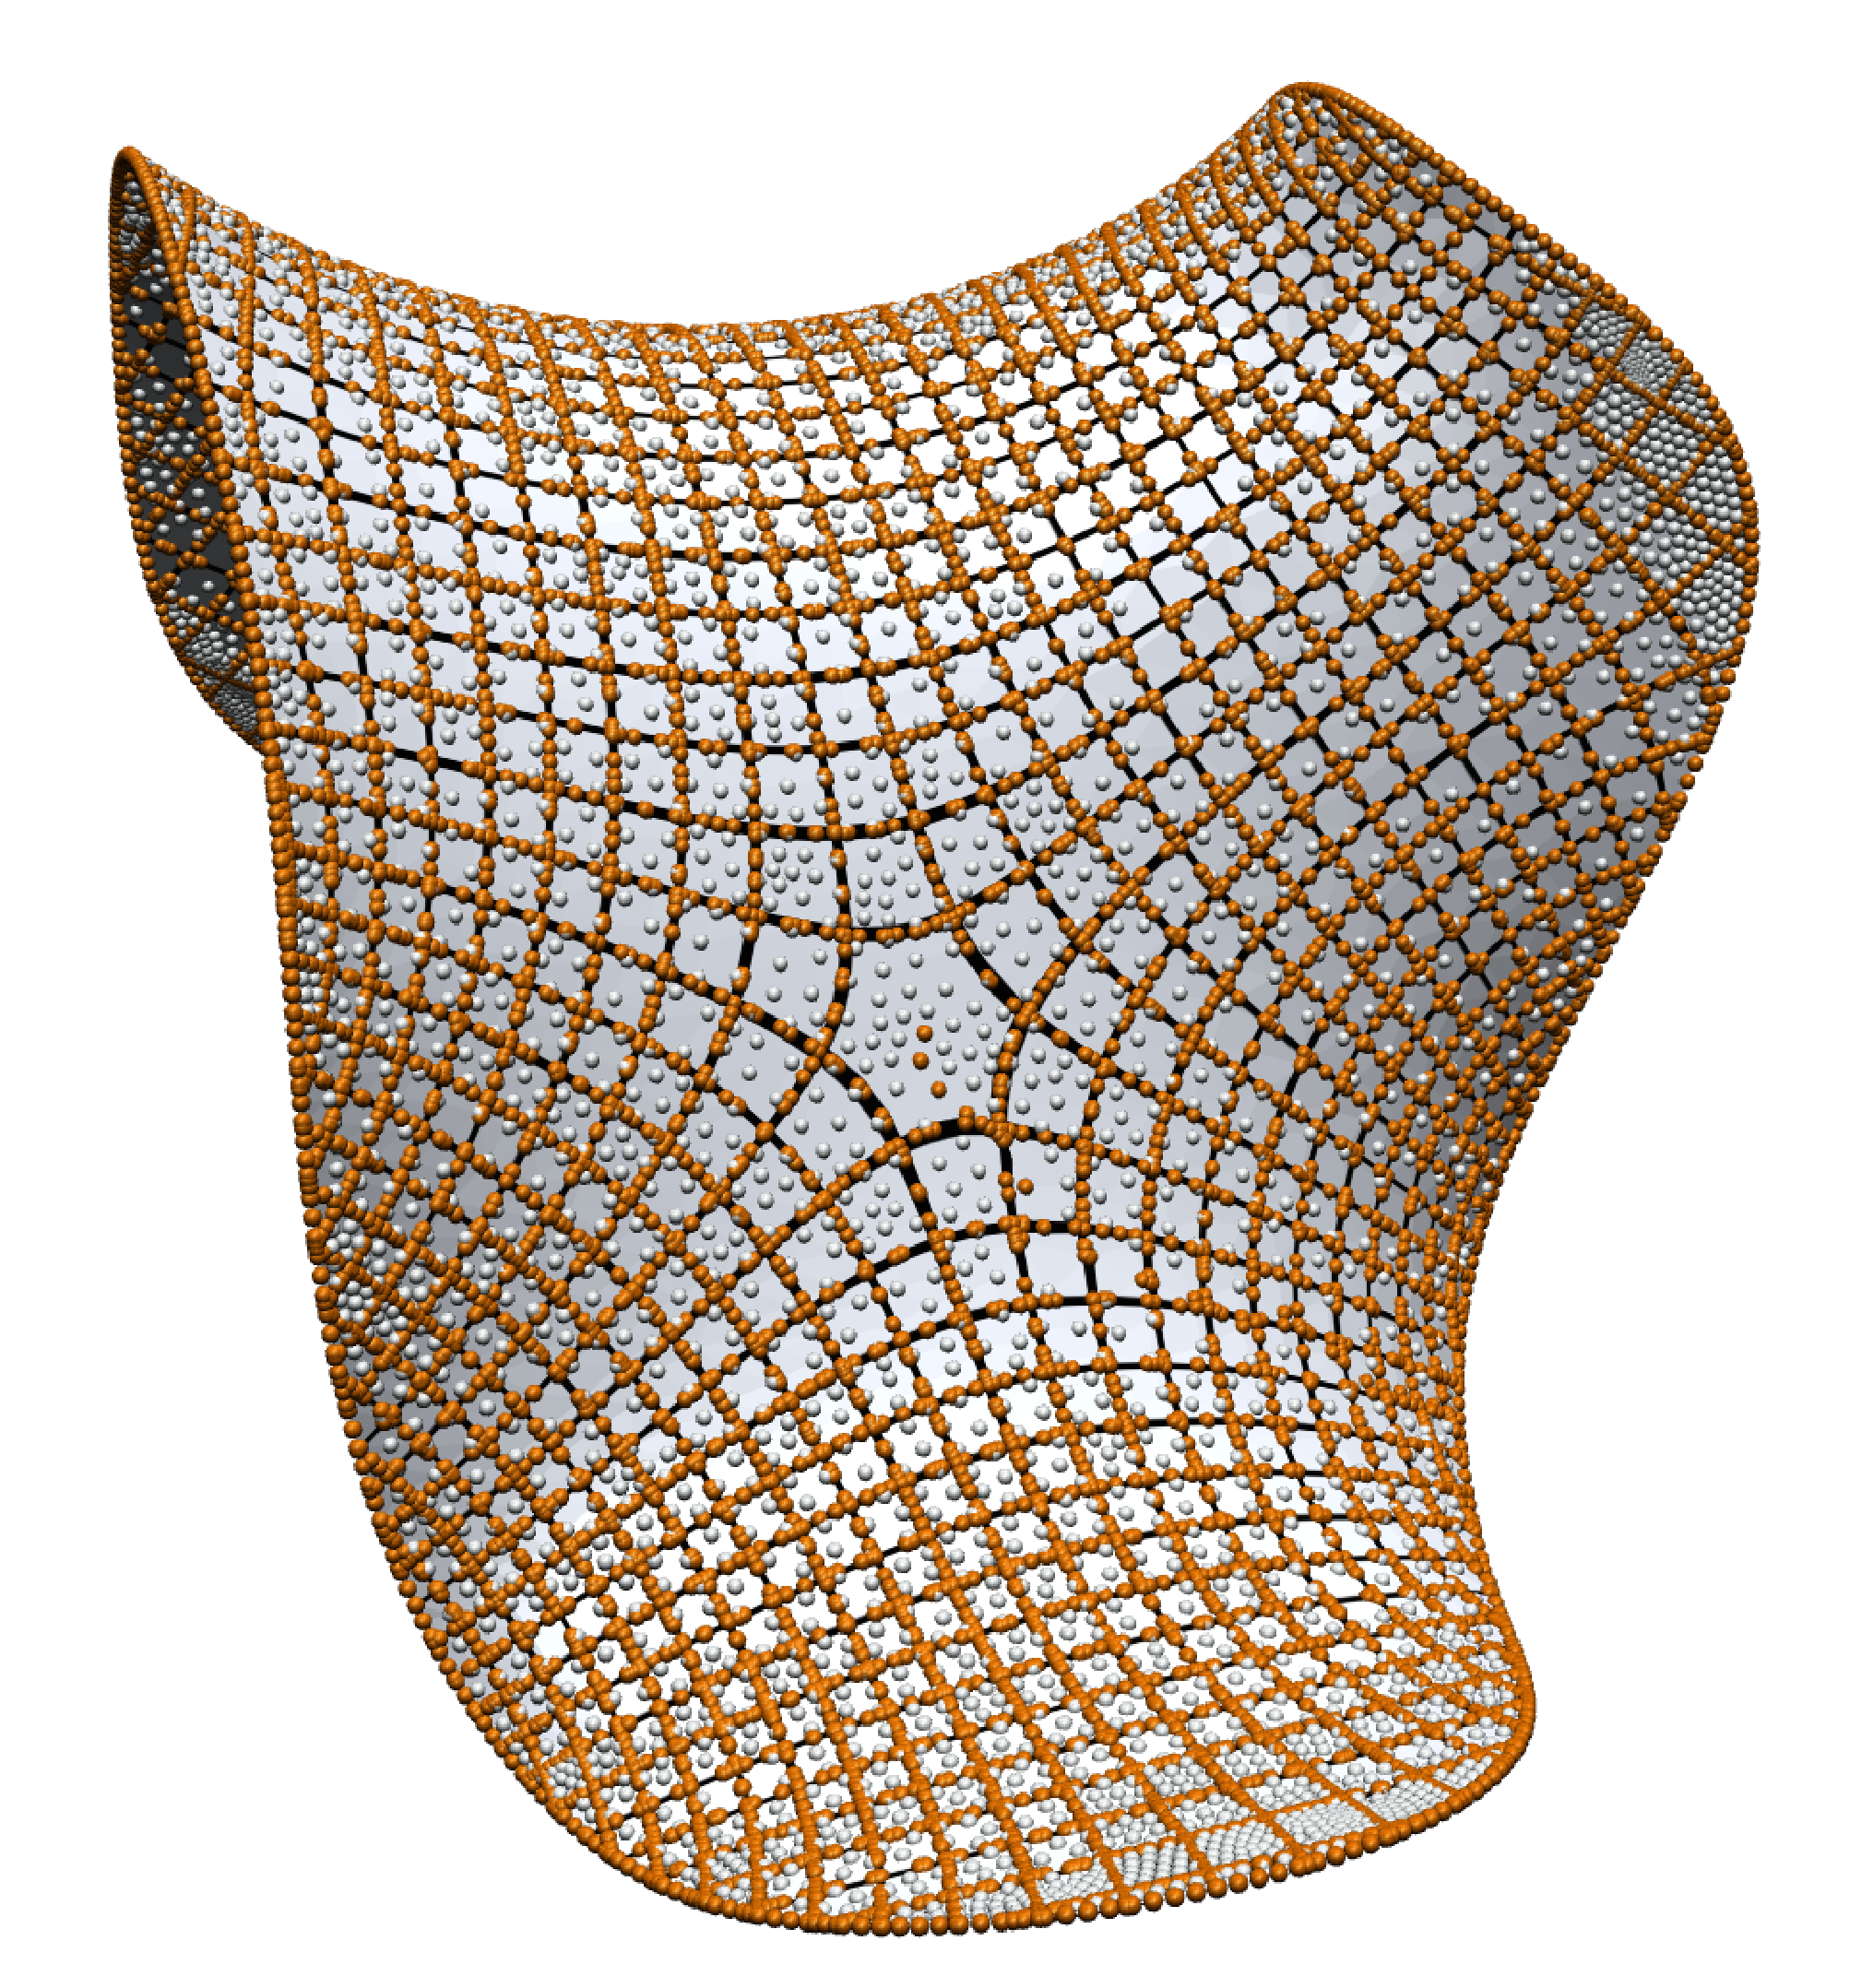
\includegraphics[width=5cm]{quasiisothermic/step06_surface.pdf}
                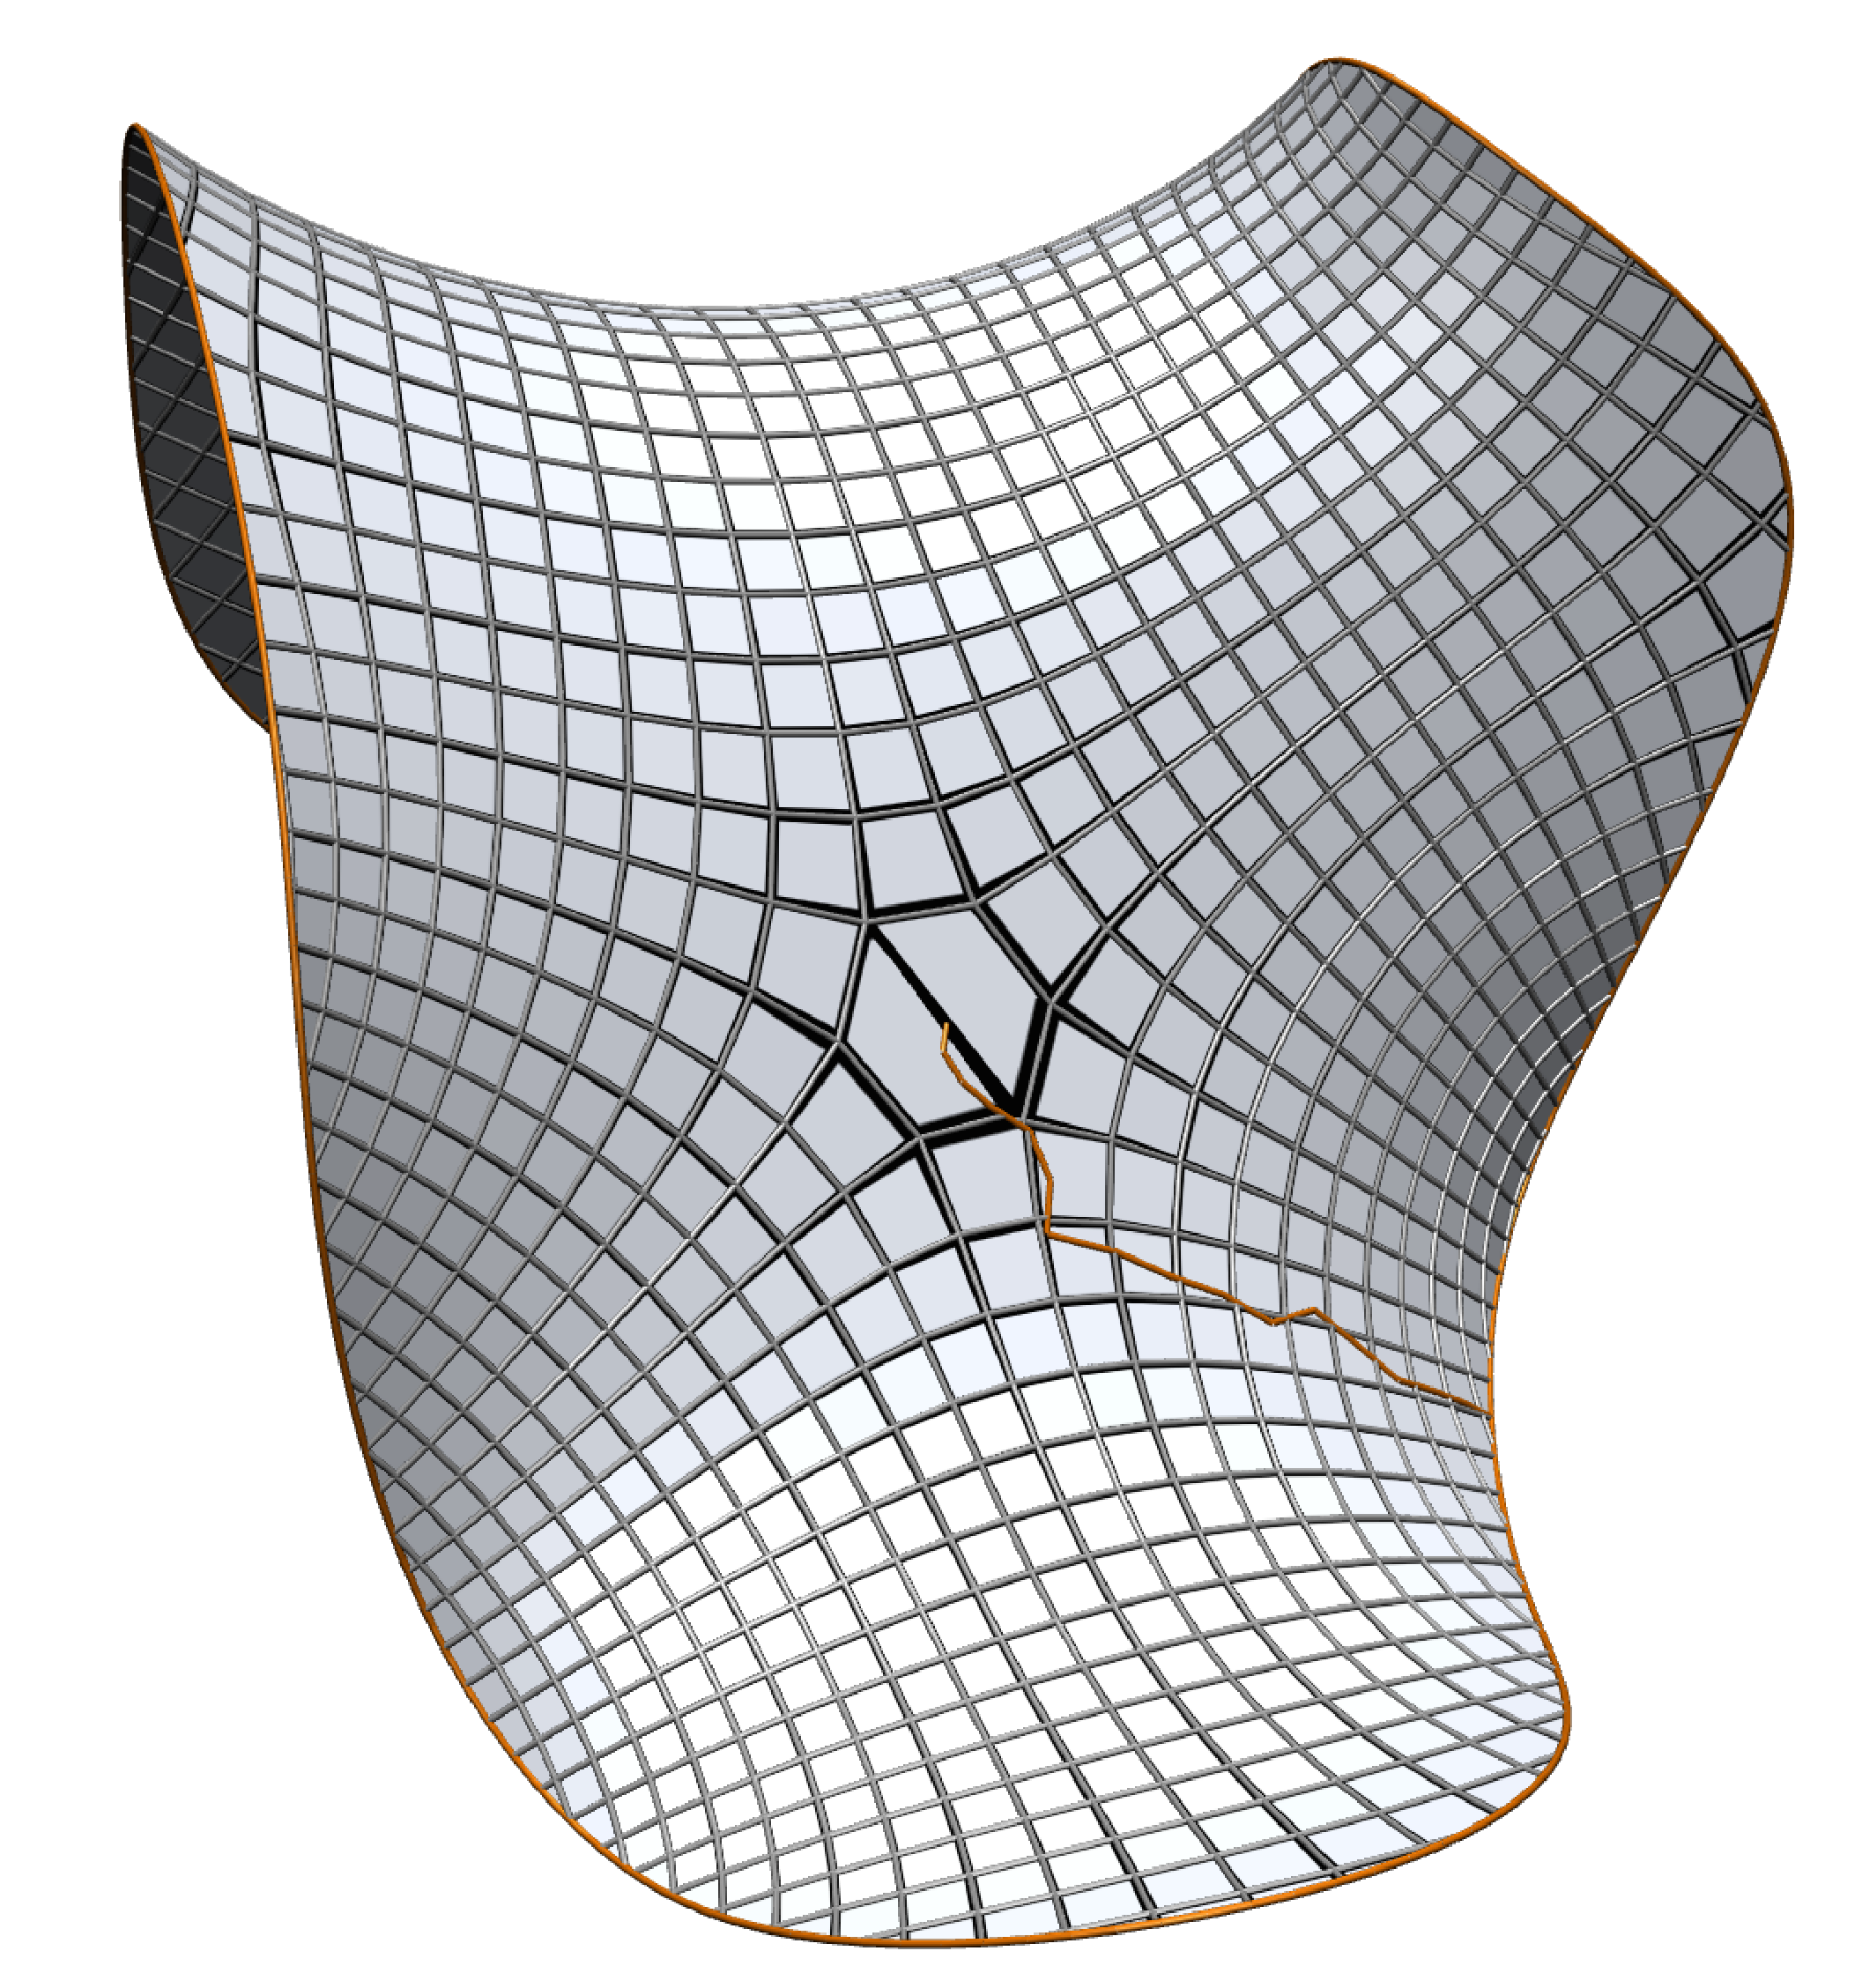
\includegraphics[width=5cm]{quasiisothermic/step07_surface.pdf}
            }
            \captionof{figure}{Three-step remeshing of the parameterized surface. Create a subdivided domain (second to left), lift this mesh to the surface (middle). Extract the new mesh from the subdivided (right).}
            \label{fig:three-step-remeshing}
\end{minipage}
\end{center}                 
            
\item[(8)] Sew up the path from the boundary to the singularity using the \emph{Topology$\to$ Stitch Cut Path} command. Select the two boundary vertices and a connected edge on the path.
\item[(9)] Remove extra vertices with the \emph{Texture Remeshing$\to$Collapse 1,2-Valent Vertices} command.
\item[(10)] Clean up the mesh from extra edges and vertices with the \emph{Selection$\to$Geodesic}, \emph{Edit$\to$Remove Edge And Fill}, and \emph{Texture Remeshing$\to$Collapse 1,2-Valent Vertices} commands.

\begin{center}
\begin{minipage}{0.9\linewidth}
            \centering
            \resizebox{\linewidth}{!}{
                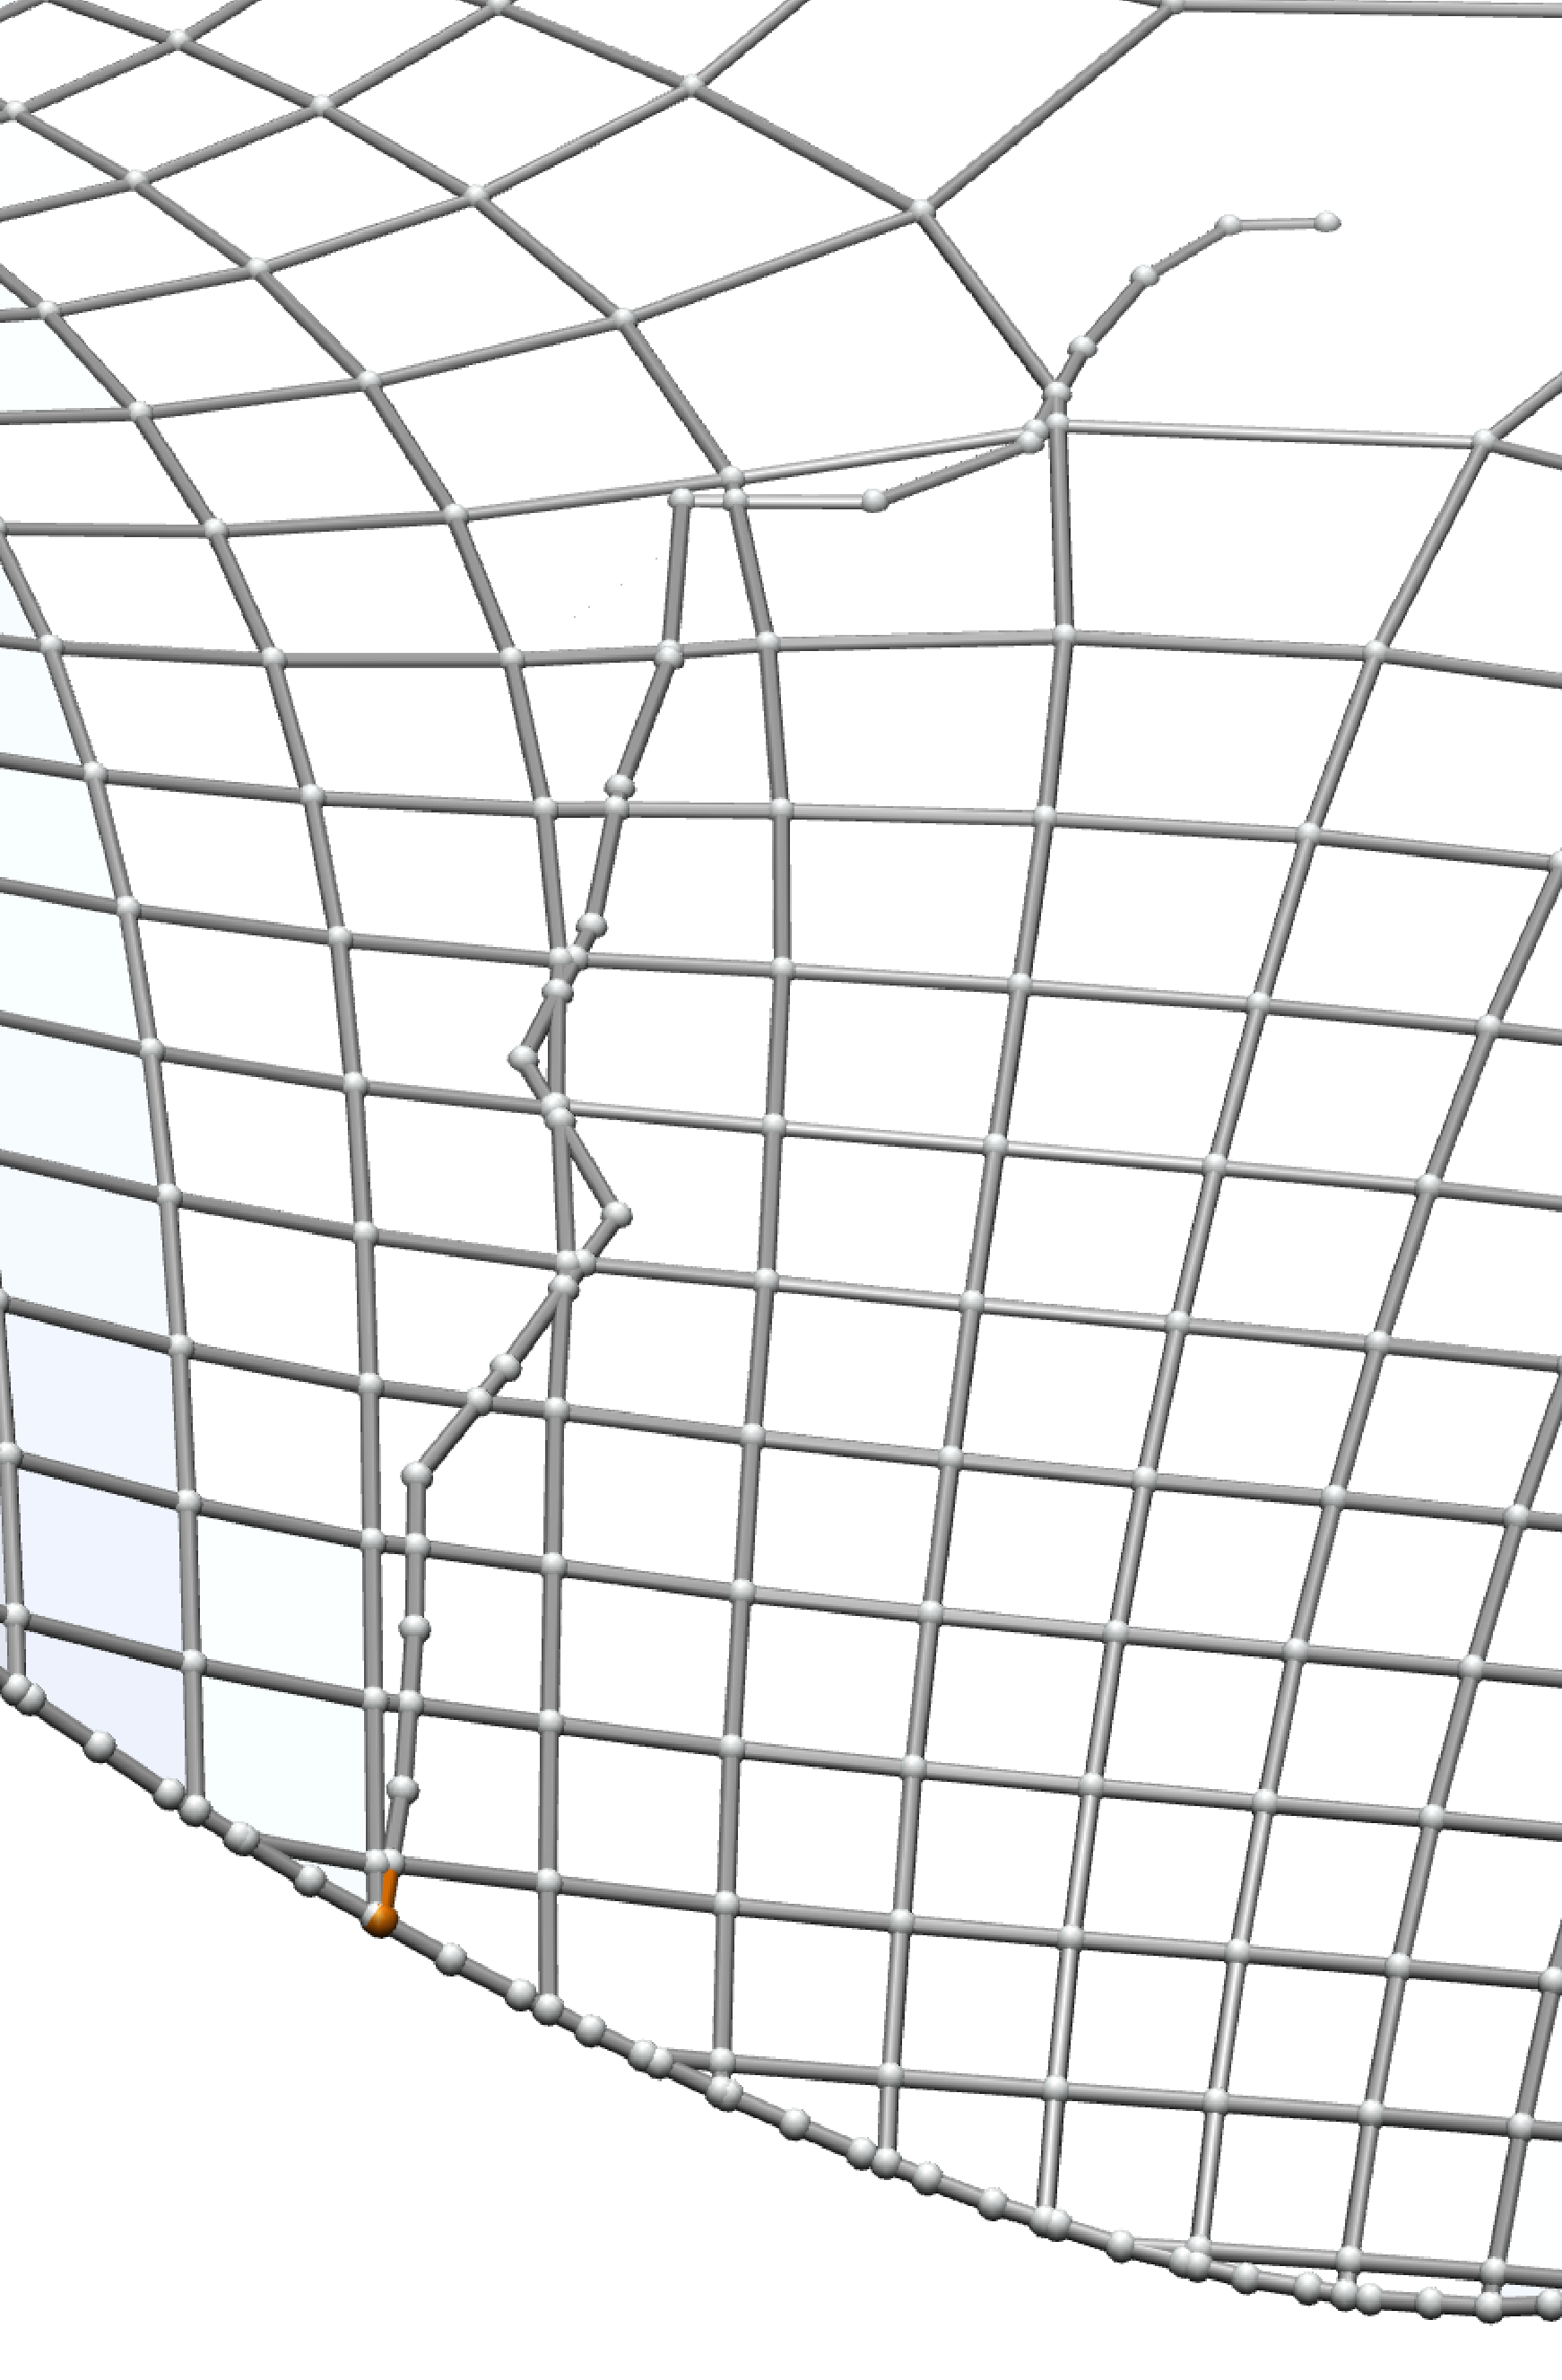
\includegraphics[width=3cm]{quasiisothermic/step08_selection.pdf}
                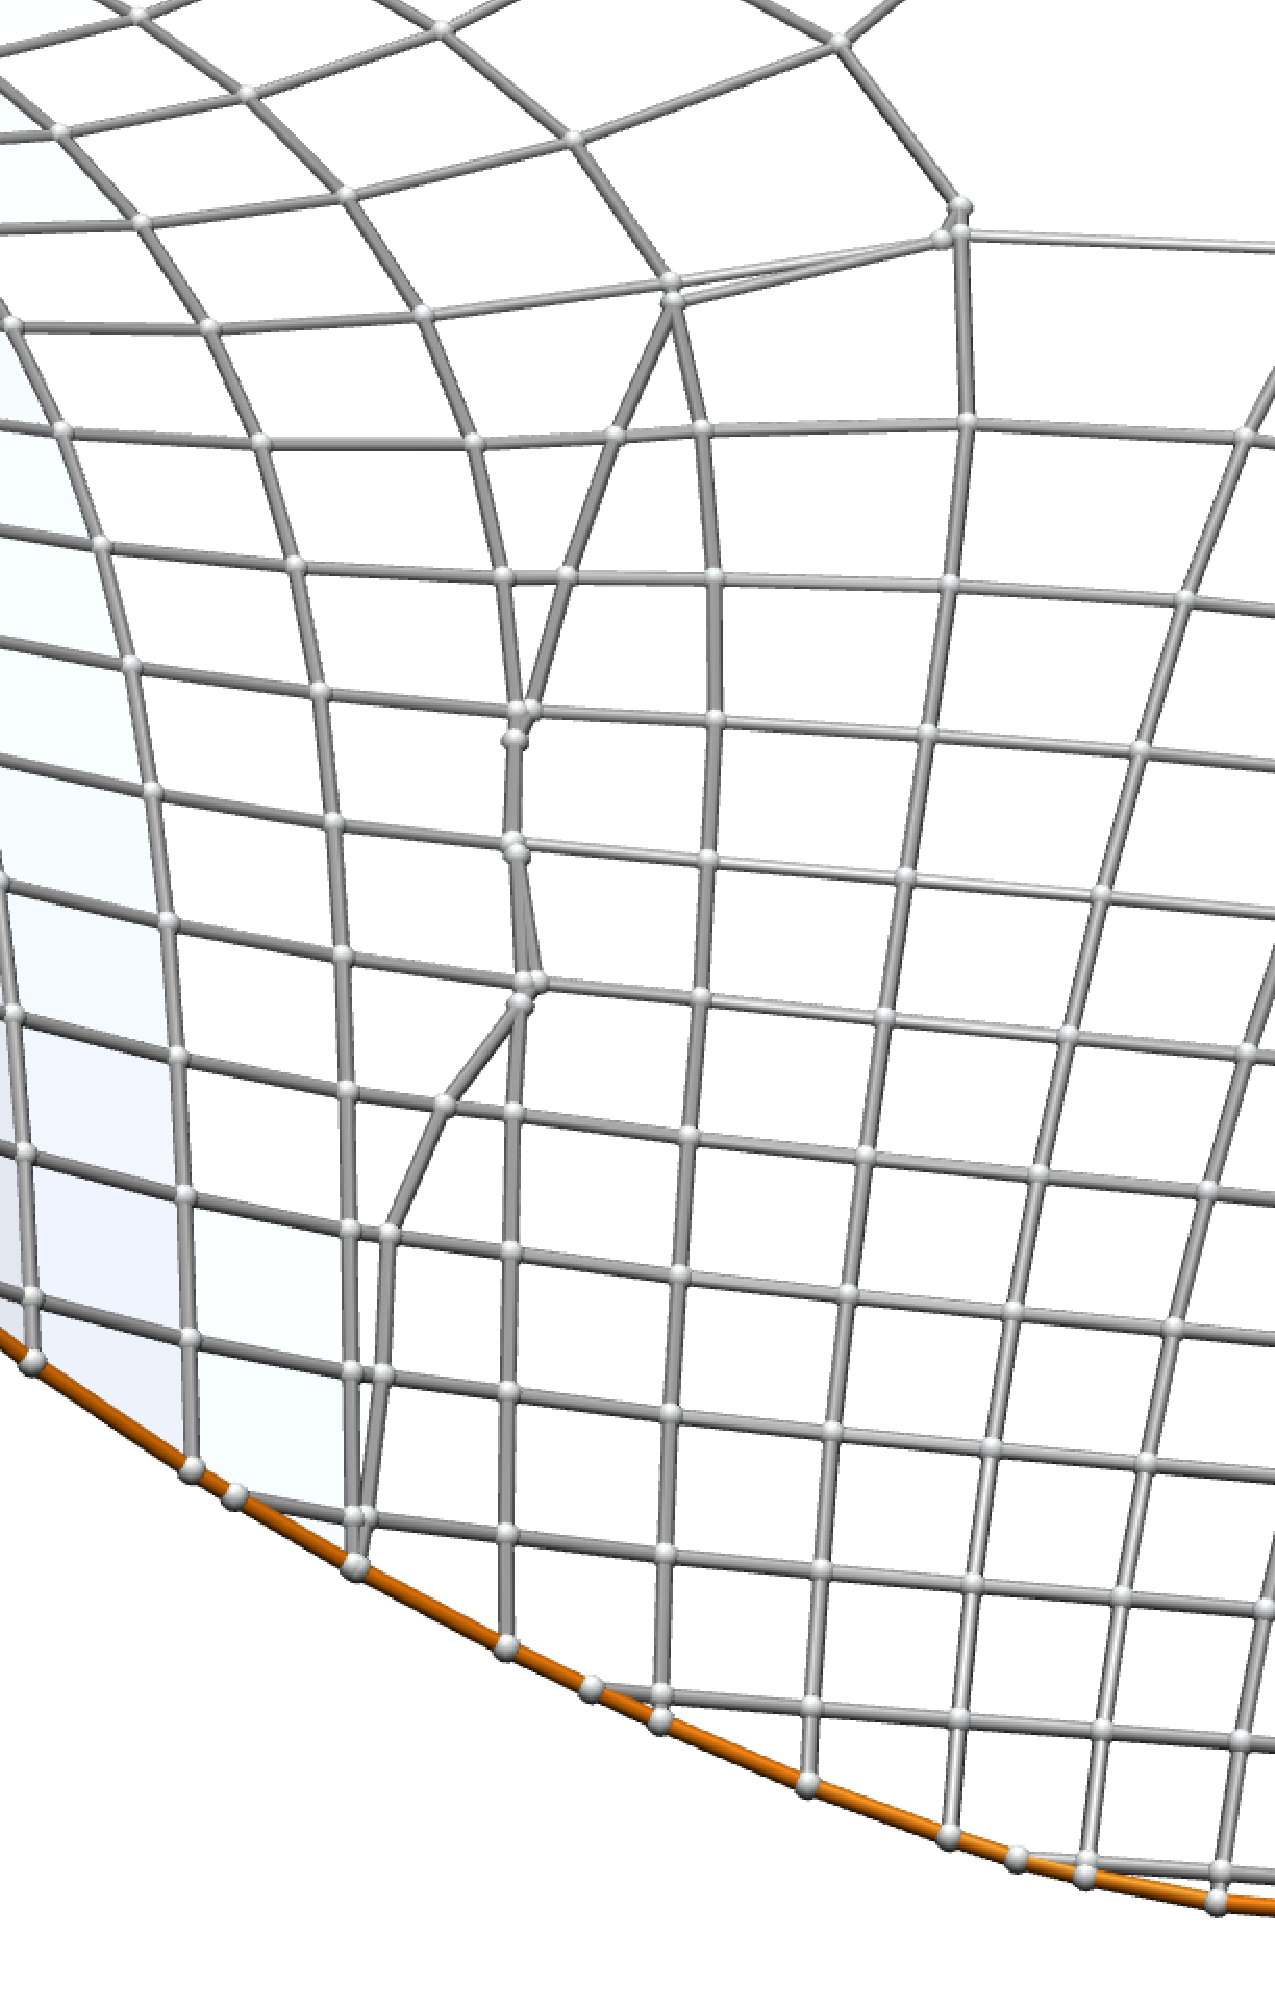
\includegraphics[width=3cm]{quasiisothermic/step09.pdf}
                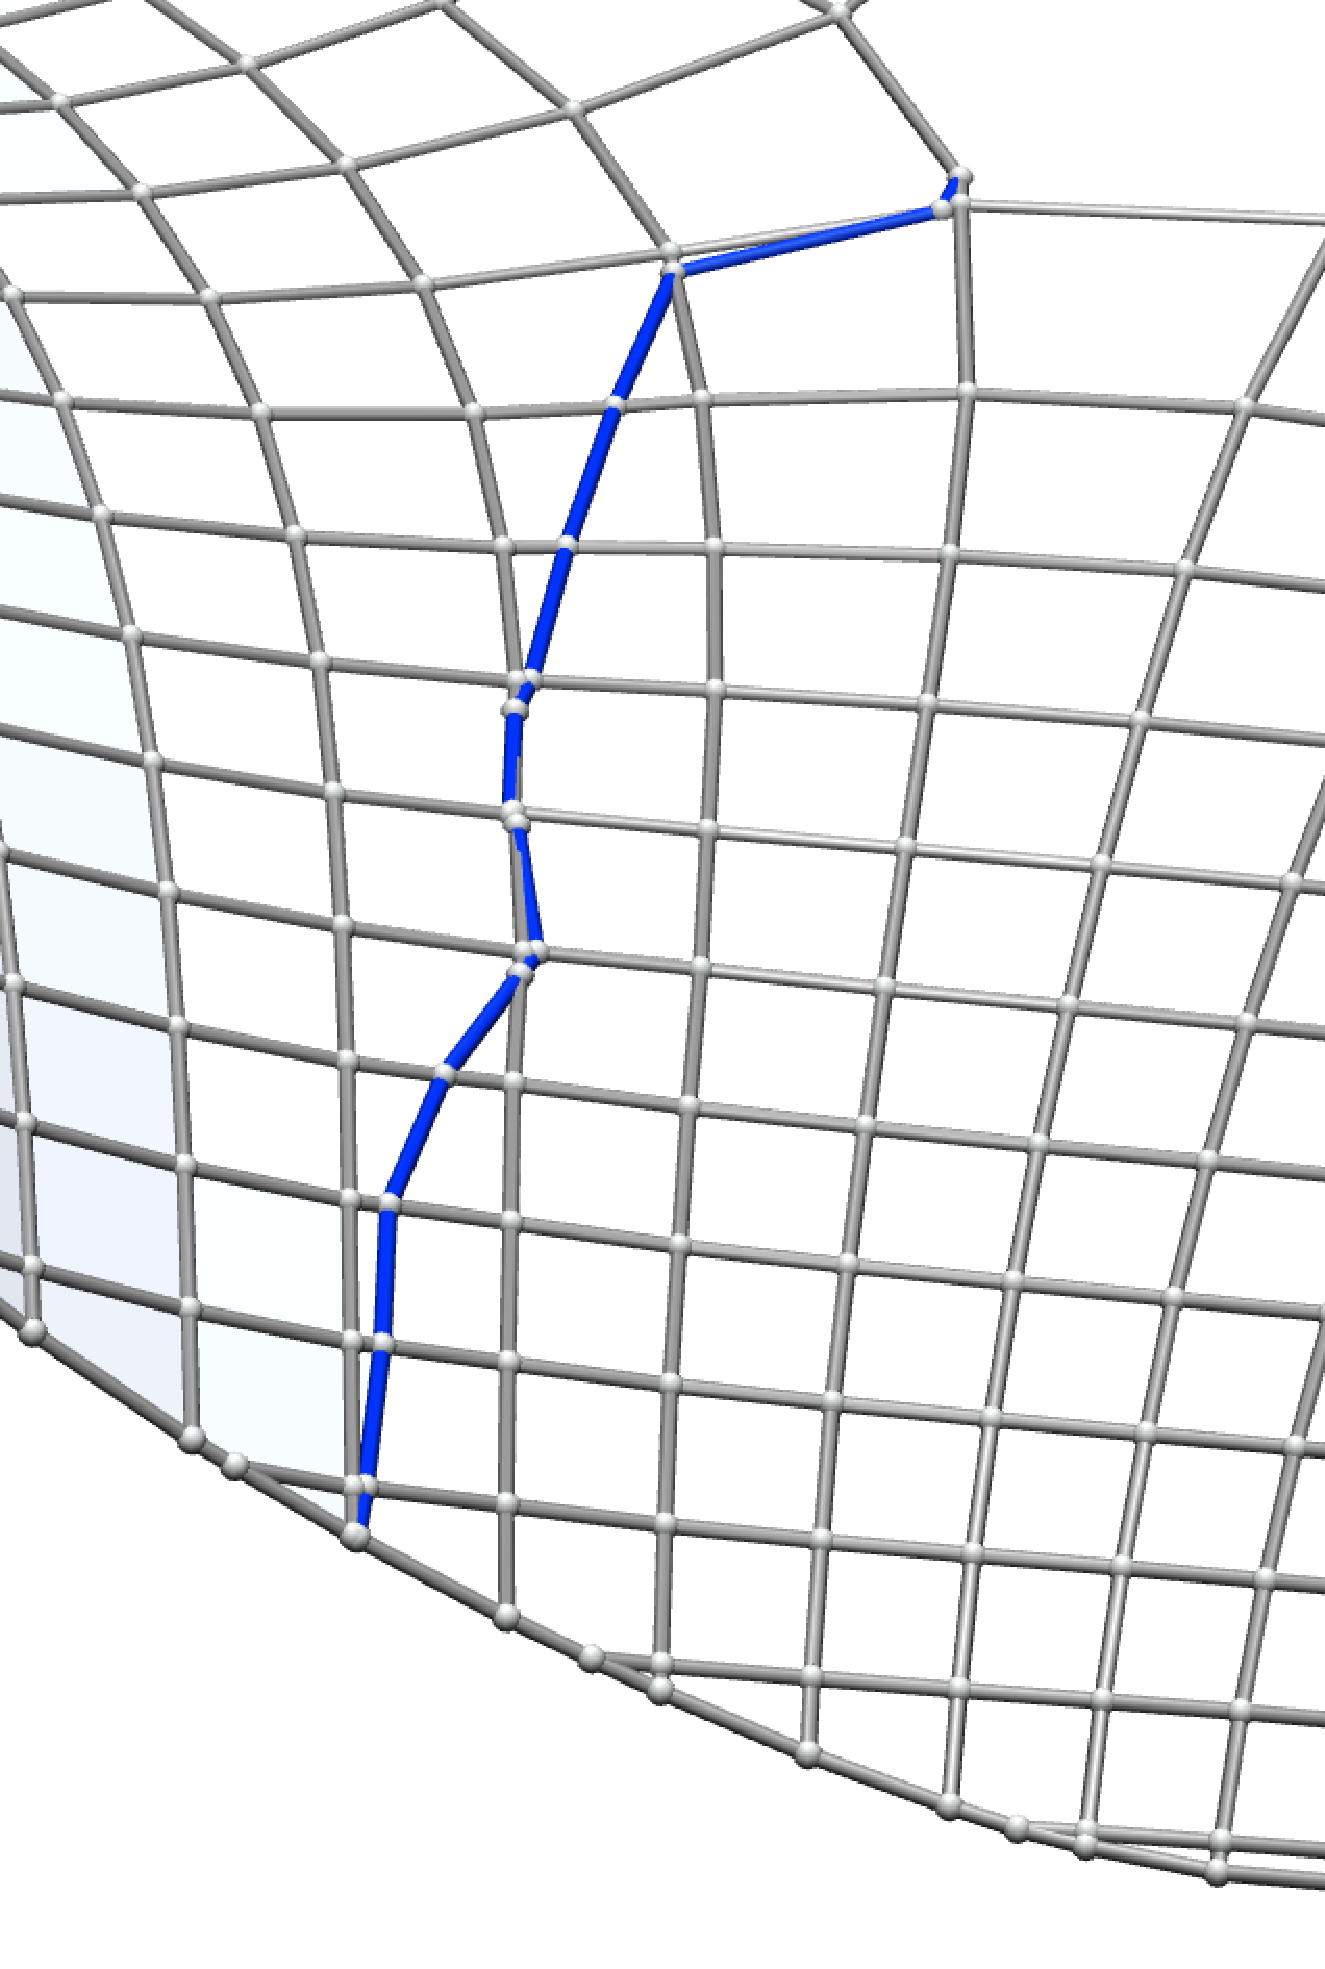
\includegraphics[width=3cm]{quasiisothermic/step10_selection.pdf}
                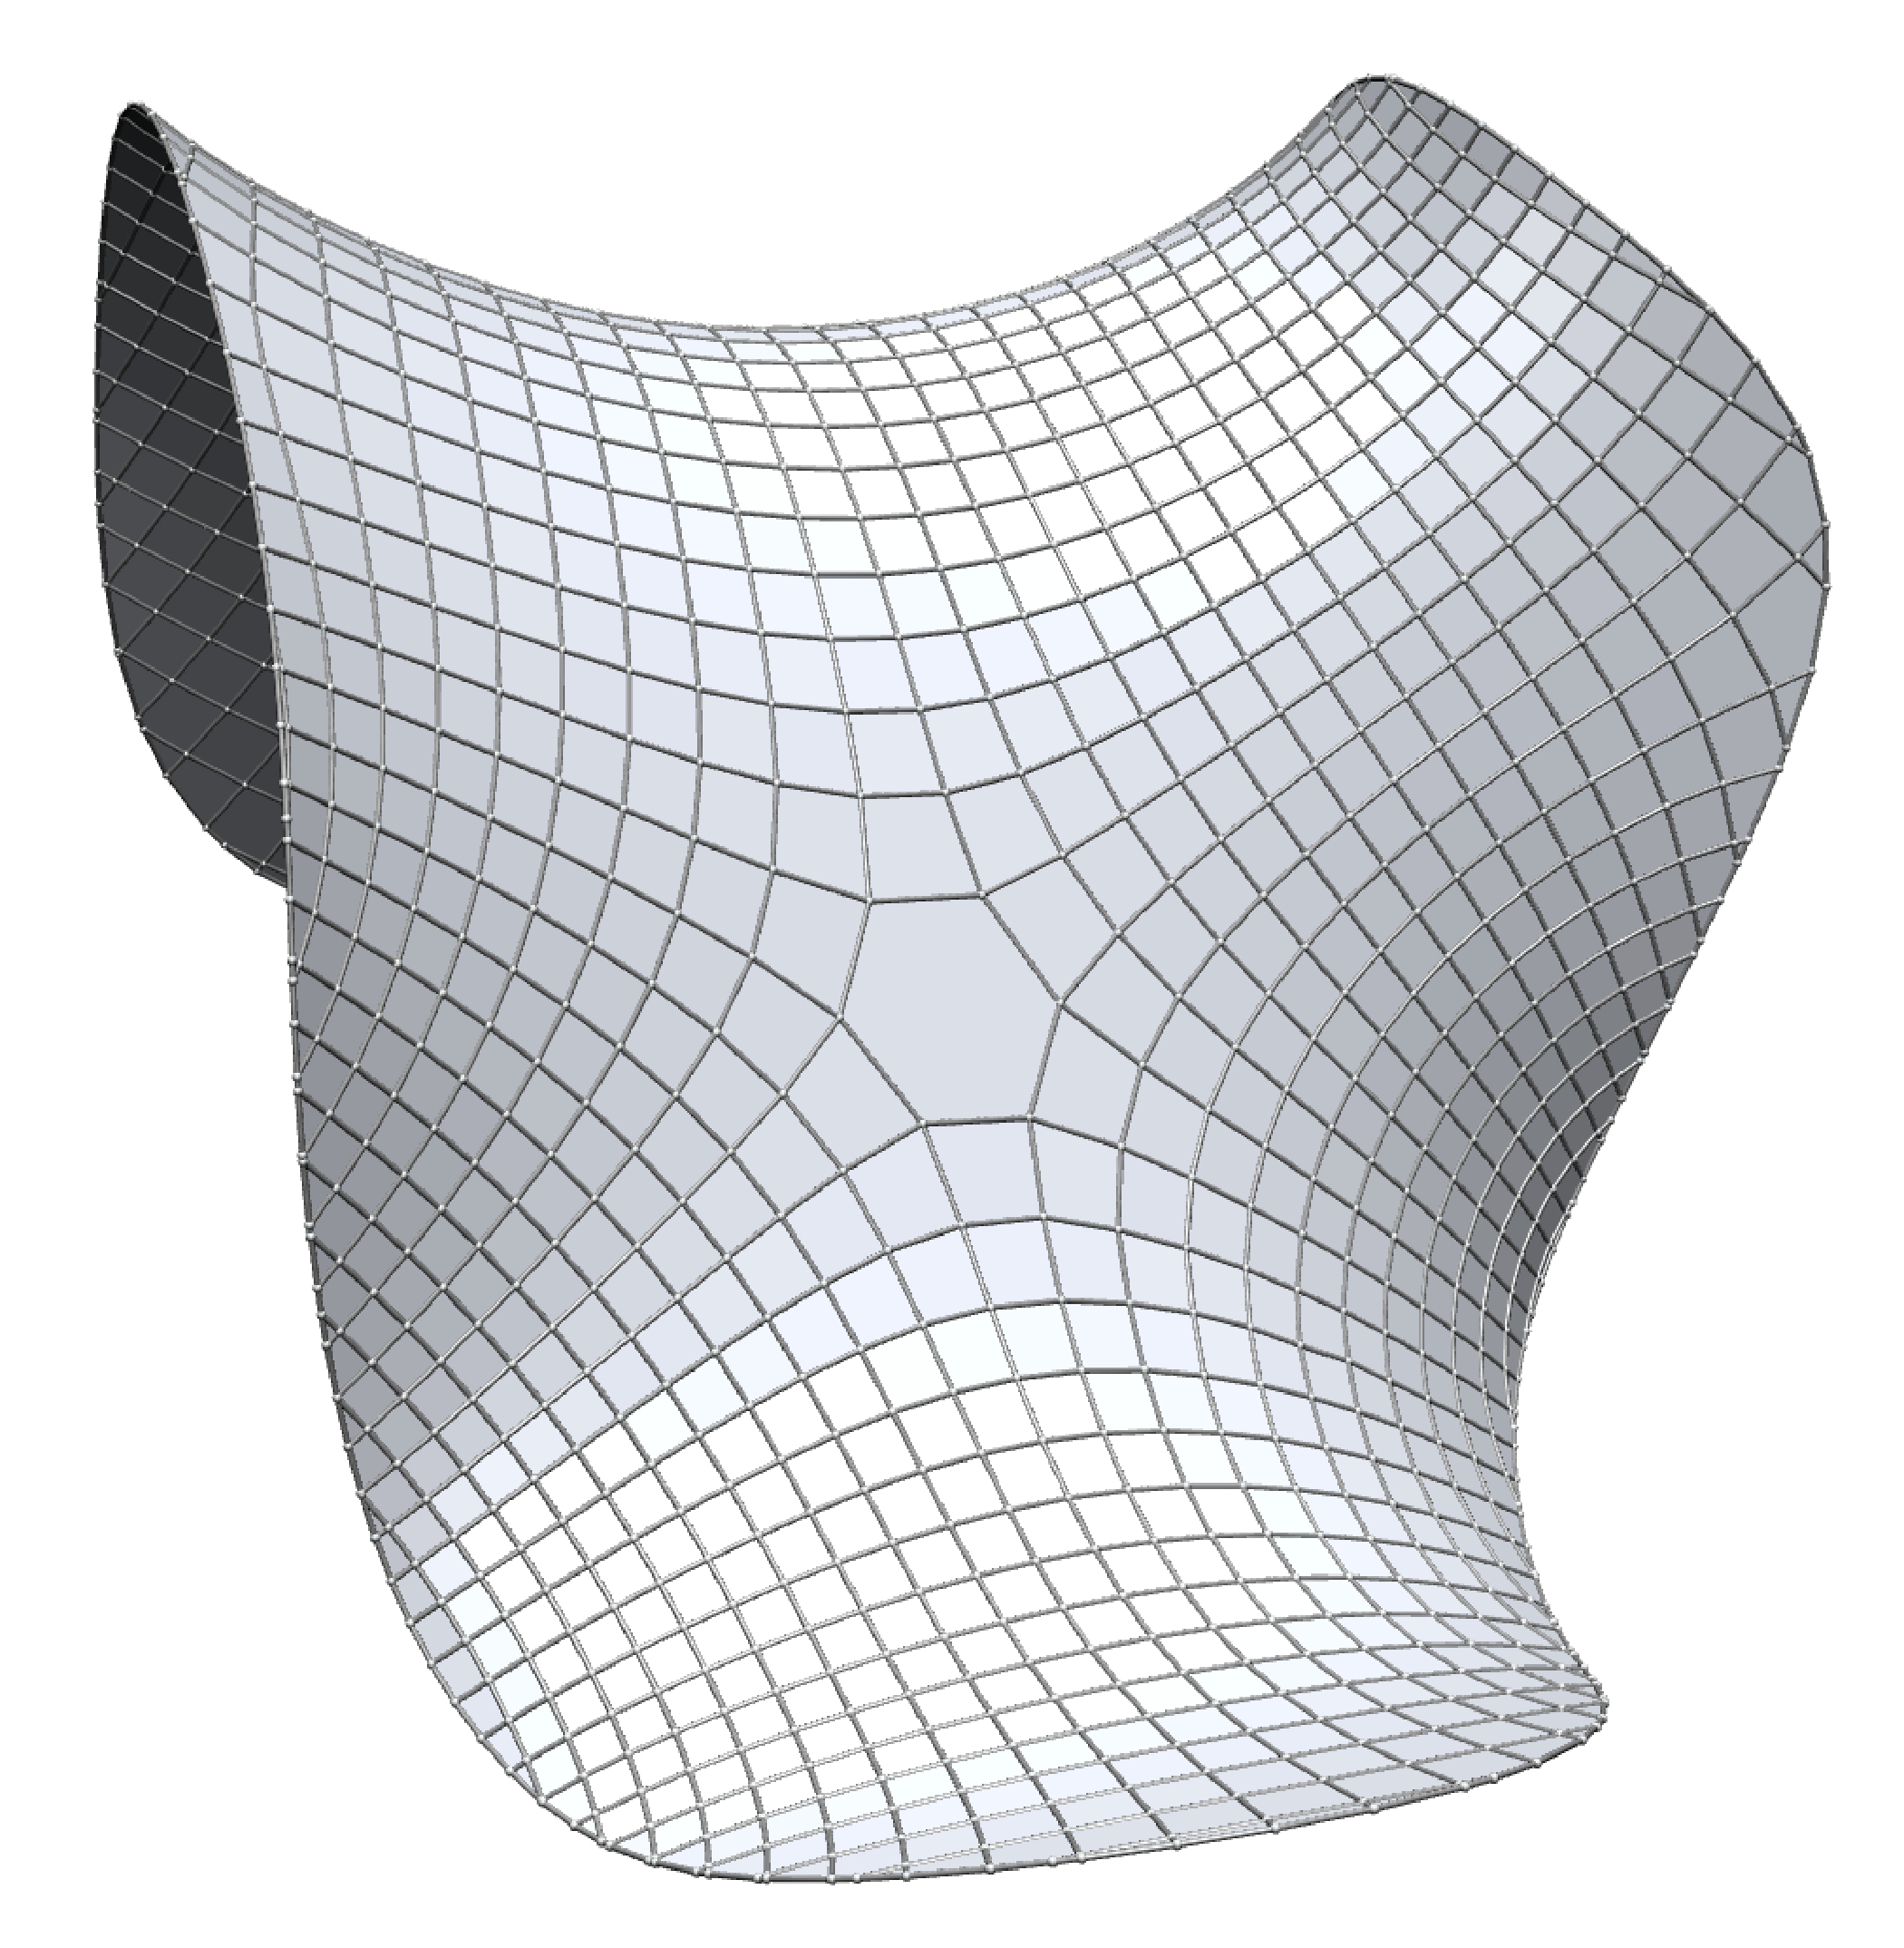
\includegraphics[width=5cm]{quasiisothermic/step10_surface.pdf}
            }
            \captionof{figure}{Removing the cut from a singularity to the boundary. Stitch the cut path by selecting the two vertices on the boundary and one adjacent edge on the path (left). Remove resulting vertices of valence $2$ (second to left). Select the path and remove extra edges.}
\end{minipage}
\end{center}    
            
\end{compactenum}

\subsection{Optimization towards touching incircles}

In Chapter~\ref{chp:quasiisothermic}, Section~\ref{sec:s-isothermic}, we propose to further optimize a new mesh to possess touching incircles, i.e., being a discrete s-isothermic mesh by definition. We propose an energy, implemented as \emph{Touching Incircles} energy, that enforces planar quadrilaterals that possess incircles to additionally possess touching incircles. Thus we superpose three energies to achieve the desired effect. Activate \emph{Incircles}, \emph{Planar Quads}, and \emph{Touching Incircles} to define the required energy.

\section{Gridshells with {\sc VaryLab}}
\label{sec:gridshells_varylab}

{\sc VaryLab} supports the creation of gridshell meshes, i.e., quadrilateral meshes with equal edge lengths. In this section we describe how the results of Chapter~\ref{chp:gridshells} were created using the features of {\sc VaryLab}.

\begin{compactenum}[(1)]

\item[(0)] Design the target surface. The surface must be a topological disk. 
\item[(1)] Create an extended reference surface.

\begin{center}
\begin{minipage}{0.9\linewidth}
            \centering
            \resizebox{0.8\linewidth}{!}{
                \includegraphics[width=3cm]{gridshells/step0_target.pdf}
                \includegraphics[width=3cm]{gridshells/step1_extended.pdf}            
            }
            \captionof{figure}{The target shape design (left) and the extended surface used as reference surface (right).}
\end{minipage}
\end{center}    

\item[(2)] Discrete conformal parameterization using isometric boundary. 

\begin{center}
\begin{minipage}{0.9\linewidth}
            \centering
            \resizebox{0.8\linewidth}{!}{
                \includegraphics[width=3cm]{gridshells/step2_0degree.pdf}
                \includegraphics[width=3cm]{gridshells/step2_40degree.pdf} 
            }
            \captionof{figure}{Conformal parameterization with orthogonal parameter lines visualized with a quadrilateral texture (left). Parameter lines sheared by $40^\circ$ (right).}
\end{minipage}
\end{center}    

\item[(3)] Create a new quadrilateral mesh using the parameterization from step 2. We are free to shear the meshing pattern in the domain by an angle $\alpha$. From the \emph{Surface Remeshing} panel we choose the \emph{Quads} mode and press \emph{Remesh}. Alternatively the three-step remeshing method can be performed, see Figure~\ref{fig:three-step-remeshing}.

\begin{center}
\begin{minipage}{0.9\linewidth}
            \centering
            \resizebox{0.8\linewidth}{!}{
                \includegraphics[width=3cm]{gridshells/step3_0degree.pdf}
                \includegraphics[width=3cm]{gridshells/step3_40degree.pdf}            
            }
            \captionof{figure}{New quadrilateral meshes with orthogonal parameter lines (left) and parameter lines sheared by $40^\circ$ (right).}
\end{minipage}
\end{center}   

\item[(4)] Remove all boundary vertices and analyze the remaining edge lengths with node colors and histogram.

\begin{center}
\begin{minipage}{0.9\linewidth}
            \centering
            \resizebox{0.9\linewidth}{!}{
                \includegraphics[width=3cm]{gridshells/step4_surface.pdf}
                \includegraphics[width=4.5cm]{gridshells/step4_hist.pdf}            
            }
            \captionof{figure}{Edge length analysis. Target edge length should be below the mean edge length.}
\end{minipage}
\end{center}   

\item[(5)] Configure the optimization using the \emph{Reference Surface} energy with the surface from step 1. Add the \emph{Springs} energy with a constant edge length depending on the size of the target surface. Finally add the \emph{Opposite Edges Curvature} energy as a fairing term and to control the local curvature of curves.

\begin{center}
\begin{minipage}{0.9\linewidth}
            \centering
            \resizebox{\linewidth}{!}{
                \includegraphics[width=5cm]{gridshells/step5_ref.pdf}
                \includegraphics[width=5cm]{gridshells/step5_equal.pdf}            
                \includegraphics[width=7cm]{gridshells/step5_hist.pdf}                            
            }
            \captionof{figure}{Reference surface visualization (left). Optimized mesh (middle). Optimized histogram (right).}
\end{minipage}
\end{center}   

\item[(6)] Run optimization. It has been proven successful to switch the reference surface energy off for a few iterations to let the mesh relax towards equal edge length and smooth parameter curves. Switching it back on will then project the mesh back onto the reference surface retaining most of the lengths and curvatures. Since the energy is non-convex there are lots of local minima and the solution depends heavily on the solver in use. The \emph{CG}, conjugate gradient, solver converges slower but yields smoother results than, e.g., the \emph{LMVM} solver.

\end{compactenum}

\subfilebibliography
\end{document}

%%% Local Variables:
%%% TeX-master: "Thesis.tex"
%%% End: